\documentclass[11pt]{article}

\usepackage[utf8]{inputenc}
\usepackage[T1]{fontenc}
\usepackage{lmodern}
\usepackage[margin=1in]{geometry}
\usepackage{amsmath,amssymb,amsthm,mathtools}
\usepackage{booktabs}
\usepackage{array}
\usepackage{enumitem}
\usepackage{xcolor}
\usepackage{tikz}
\usetikzlibrary{arrows.meta,positioning,calc,decorations.pathreplacing,fit,backgrounds,shapes.geometric}
\usepackage{microtype}
\usepackage{listings}
\usepackage{fancyvrb}
\usepackage{hyperref}

% Unicode symbols occurring in quoted Lean 4 statements (pdflatex + inputenc utf8).
\DeclareUnicodeCharacter{2203}{\ensuremath{\exists}}
\DeclareUnicodeCharacter{2200}{\ensuremath{\forall}}
\DeclareUnicodeCharacter{2115}{\ensuremath{\mathbb{N}}}
\DeclareUnicodeCharacter{00D7}{\ensuremath{\times}}
\DeclareUnicodeCharacter{0393}{\ensuremath{\Gamma}}
\DeclareUnicodeCharacter{039B}{\ensuremath{\Lambda}}
\DeclareUnicodeCharacter{03C3}{\ensuremath{\sigma}}
\DeclareUnicodeCharacter{2227}{\ensuremath{\wedge}}
\DeclareUnicodeCharacter{2080}{\ensuremath{{}_0}}
\DeclareUnicodeCharacter{2081}{\ensuremath{{}_1}}
\DeclareUnicodeCharacter{2082}{\ensuremath{{}_2}}
\DeclareUnicodeCharacter{2265}{\ensuremath{\ge}}
\DeclareUnicodeCharacter{2264}{\ensuremath{\le}}
\DeclareUnicodeCharacter{2192}{\ensuremath{\to}}
\DeclareUnicodeCharacter{00B7}{\ensuremath{\cdot}}
\DeclareUnicodeCharacter{230A}{\ensuremath{\lfloor}}
\DeclareUnicodeCharacter{230B}{\ensuremath{\rfloor}}
\DeclareUnicodeCharacter{2212}{\ensuremath{-}}
\DeclareUnicodeCharacter{2243}{\ensuremath{\simeq}}

\emergencystretch=1.5em

\hypersetup{
  pdftitle={Integer multiplication in O(n log n) time on a single two-dimensional grid, with a machine-checked proof},
  pdfauthor={Piaoyang Cui, Yiming Liu, David P. Woodruff},
  colorlinks=true,
  linkcolor=black,
  citecolor=black,
  urlcolor=black
}

\lstset{
  basicstyle=\ttfamily\scriptsize,
  columns=fullflexible,
  keepspaces=true,
  breaklines=true,
  frame=single,
  rulecolor=\color{black!25},
  backgroundcolor=\color{black!3},
  keywordstyle=\bfseries,
  commentstyle=\itshape\color{black!65},
  showstringspaces=false
}

\newtheorem{maintheorem}{Theorem}
\newtheorem*{thmmainrestated}{Theorem~\ref{thm:main} \normalfont(restated)}
\newtheorem{theorem}{Theorem}[section]
\newtheorem{lemma}[theorem]{Lemma}
\newtheorem{proposition}[theorem]{Proposition}
\newtheorem{corollary}[theorem]{Corollary}
\newtheorem{fact}[theorem]{Fact}
\theoremstyle{definition}
\newtheorem{definition}[theorem]{Definition}
\theoremstyle{remark}
\newtheorem{remark}[theorem]{Remark}

% Mathematical macros
\newcommand{\C}{\mathbb{C}}
\newcommand{\R}{\mathbb{R}}
\newcommand{\Z}{\mathbb{Z}}
\newcommand{\Q}{\mathbb{Q}}
\newcommand{\N}{\mathbb{N}}
\newcommand{\Cg}{\widetilde{\mathbb{C}}}
\newcommand{\Rg}{\widetilde{\mathbb{R}}}
\newcommand{\Rr}{\mathcal{R}}
\newcommand{\cA}{\mathcal{A}}
\newcommand{\cB}{\mathcal{B}}
\newcommand{\cO}{\mathcal{O}}
\newcommand{\sinc}{\operatorname{sinc}}
\newcommand{\erf}{\operatorname{erf}}
\newcommand{\erfc}{\operatorname{erfc}}
\newcommand{\RM}{\operatorname{RM}}
\newcommand{\RD}{\operatorname{RD}}
\newcommand{\Pack}{\operatorname{Pack}}
\newcommand{\Quant}{\mathcal{Q}}
\newcommand{\ord}{\operatorname{ord}}
\newcommand{\eps}{\varepsilon}

\title{\textbf{Integer multiplication in $O(n\log n)$ time on a single two-dimensional grid,\\ with a machine-checked proof}\thanks{This work was carried out with substantial assistance from AI agents (Gemini~4 and other models), including proof development, auditing, and the Lean~4 formalization; see Section~\ref{sec:intro-verification}.}}
\author{%
  \begin{tabular}[t]{@{}c@{}}
    Piaoyang Cui\thanks{Authors are listed in alphabetical order.}\\[0.4ex]
    {\normalsize Google DeepMind}
  \end{tabular}%
  \hspace{2.6em}%
  \begin{tabular}[t]{@{}c@{}}
    Yiming Liu\textsuperscript{\normalfont$\dagger$}\\[0.4ex]
    {\normalsize Google DeepMind}
  \end{tabular}%
  \hspace{2.6em}%
  \begin{tabular}[t]{@{}c@{}}
    David P. Woodruff\textsuperscript{\normalfont$\dagger$}\\[0.4ex]
    {\normalsize Google Research}\\[-0.2ex]
    {\normalsize Carnegie Mellon University}
  \end{tabular}%
}
\date{30 September 2026}

\begin{document}
\hypersetup{pageanchor=false}
\maketitle
\thispagestyle{empty}

\begin{abstract}
We give an algorithm that multiplies two $n$-bit integers in $O(n\log n)$ steps on a deterministic multitape Turing machine, together with a machine-checked (Lean~4) proof of an $O(n\log n)$ step bound for an explicit eight-stack machine. The algorithm of Harvey and van der Hoeven reaches the same bound by routing a one-dimensional Fourier transform through a multidimensional transform of pairwise coprime lengths, which requires Chinese remaindering and a resampling step between grids of different sizes. Our algorithm works on a single two-dimensional power-of-two grid of the same size as the transform it computes. Cooley--Tukey twiddle factors are read as fractional row shifts. Each row is spread by a data-independent sinc-Gaussian kernel, the two-dimensional transform is computed by a multiplication-free polynomial transform and recursive one-dimensional transforms, and the spreading is undone by a two-term recurrence per column whose conditioning is uniform. Because the kernel's passband stays flat up to the Nyquist frequency, the working precision grows only additively along the recursion. A single-threaded C implementation using GMP for inner products agrees bit for bit with GMP on all tested inputs (one random operand pair per size, up to a billion bits), while running over a hundred times slower.
\end{abstract}


\newpage
\hypersetup{pageanchor=true}
\setcounter{page}{1}

\section{Introduction}\label{sec:intro}

\subsection{Background}\label{sec:intro-background}

Fourier-based integer multiplication splits two $n$-bit nonnegative integers $A$ and $B$ into $N = \lceil n / b \rceil$ radix-$2^b$ digits of $b = \Theta(\log n)$ bits. It chooses a transform length $R_0 = \Theta(n / \log n)$ with $R_0 \ge 2N$ and evaluates a cyclic convolution of length $R_0$ at fixed-point precision $p_0 = \Theta(\log n)$ bits. A one-dimensional radix-2 discrete Fourier transform (DFT) of length $R_0$ performs $\frac{1}{2} R_0 \log_2 R_0$ complex butterfly multiplications on $p_0$-bit operands. If each $p_0$-bit product costs $\mathsf{M}(p_0)$ steps, these twiddle multiplications alone cost $\Theta(R_0 \log R_0 \cdot \mathsf{M}(p_0)) = \Theta(n \cdot \mathsf{M}(\log n))$ steps, an extra factor of $\Theta(\log \log n)$ over $n \log n$ when $\mathsf{M}(p) = \Theta(p \log p)$~\cite{HvdH21}. Sch\"onhage and Strassen~\cite{SS71} achieved $O(n \log n \log \log n)$ steps on a multitape Turing machine by working in Fermat quotient rings $\Z / (2^{2^k}+1)\Z$. F\"urer~\cite{Furer07,Furer09} reduced the $\log \log n$ factor to $2^{O(\log^* n)}$ using synthetic roots in cyclotomic rings, and Harvey, van der Hoeven, and Lecerf~\cite{HvdHL16} sharpened that bound to $O(n \log n \cdot 8^{\log^* n})$ unconditionally.

A classical algebraic tool for eliminating butterfly multiplications is the polynomial transform of Nussbaumer and Quandalle~\cite{NQ79,Nussbaumer80,Nussbaumer82}. In the negacyclic quotient ring $\Rr_r := \C[y]/(y^r + 1)$ where $r$ is a power of two, the indeterminate $y$ satisfies $y^r \equiv -1$ and has multiplicative order $2r$. Multiplying an element of $\Rr_r$ by any power of $y$ is a signed cyclic shift of its $r$ complex coefficients and requires zero scalar multiplications. Combined with negacyclic-to-cyclic weighting~\cite{SS71,CF94}, a polynomial transform of length $t_1$ over $\Rr_r$ ($t_1 \mid r$) reduces a two-dimensional transform $F_{t_1, r}$ to $t_1$ one-dimensional transforms $F_r$ and an odd-stride permutation~\cite{NQ79,Nussbaumer82}. Integer multiplication, however, requires a one-dimensional transform $F_{t_1 r}$, which differs from $F_{t_1, r}$ by the Cooley--Tukey twiddle factors $e^{2\pi i j_1 u_2 / (t_1 r)}$.

Harvey and van der Hoeven~\cite{HvdH21} achieved $O(n \log n)$ steps by bridging one-dimensional and power-of-two multidimensional transforms through Chinese remaindering. Their algorithm routes the length-$R$ transform through a $d$-dimensional Good--Thomas transform of pairwise coprime lengths and resamples each axis to a power-of-two length by Gaussian convolution, a step related to nonuniform Fourier transform (NUFFT) gridding~\cite{DR93,PST01,GL04,BMK19}. Like the present paper, it evaluates the resulting power-of-two multidimensional transforms by Nussbaumer's polynomial transforms~\cite{NQ79,Nussbaumer80,Nussbaumer82}. The proof of their main theorem takes $d = 1729$~\cite{HvdH21}. Because the source length and target power-of-two length on each axis differ, the resampling offset varies across every coordinate index and expands the grid at each recursive step. A recent preprint~\cite{OAI26} gives an $O(n(\log n)^{1-\kappa})$ algorithm on a multitape Turing machine by combining a Harvey--van der Hoeven-style architecture with finite linear network primitives; the present paper does not use it.

\subsection{Main results}\label{sec:intro-results}

We show that $O(n \log n)$ integer multiplication requires neither Chinese remaindering nor resampling between grids of different sizes. Instead, we relate $F_{t_1 r}$ and $F_{t_1, r}$ directly on a single two-dimensional power-of-two grid $R = t_1 r$. Throughout, an $n$-bit integer means a nonnegative integer in $[0, 2^n)$ (signed $n$-bit integers reduce immediately in $O(n)$ steps).

\begin{maintheorem}\label{thm:main}
There is a deterministic multitape Turing machine and a constant $C > 0$ such that, for every $n \ge 2$ and any two $n$-bit integers $A$ and $B$, given the binary representations of $A$ and $B$ on the input tape, the machine writes the $2n$-bit binary product on the output tape in at most $C n \log_2 n$ steps.
\end{maintheorem}

The machine of Theorem~\ref{thm:main} has the following structural properties. Every Fourier transform it performs has power-of-two length, and each top-level transform of length $R_0 = \Theta(n / \log n)$ recurses on $t_{1,\ell} \times r_\ell$ sub-grids of the same total size ($R_\ell = t_{1,\ell} r_\ell$) with no grid expansion, no Chinese remainder map, no prime transform length, and no resampling between grids of different sizes. Inner products of $O((\log n)^2)$-bit integers are delegated to the same algorithm one level down, backed at the bottom stage by a one-dimensional radix-2 Fourier multiplier using schoolbook arithmetic.

\begin{maintheorem}[machine-checked]\label{thm:lean}
A fixed stack machine \texttt{tmIntMul} (Mathlib's \texttt{Turing.FinTM2}: eight binary stacks, $32$ register states, a fixed finite control) satisfies the following, verified in Lean~4~\cite{dMU21,Mathlib20}. For every $n \ge 2$ and all $A, B < 2^n$, started with the $2n$ input bits it halts with the $2n$ bits of $A \cdot B$ on its output stack within $C \cdot n \lfloor \log_2 n \rfloor$ steps, for a constant $C$ (the formal statement is existential; its proof exhibits the explicit witness \texttt{C\_tm\_total} $\approx 5\cdot 10^{92}$, Section~\ref{sec:lean}, \texttt{IntMul.\allowbreak tmIntMul\_\allowbreak evalsToInTime\_\allowbreak n\_\allowbreak log\_\allowbreak n}). Every step executes $O(1)$ elementary stack operations (\texttt{IntMul.\allowbreak tmIntMul\_\allowbreak elementary\_\allowbreak stack\_\allowbreak ops\_\allowbreak n\_\allowbreak log\_\allowbreak n}). The proof uses no axioms beyond \texttt{propext}, \texttt{Classical.choice}, and \texttt{Quot.sound}.
\end{maintheorem}

\begin{table}[ht]
\centering
\small
\caption{Comparison of transform components in~\cite{HvdH21} and in this paper.}
\label{tab:components}
\setlength{\tabcolsep}{6pt}
\begin{tabular}{@{}>{\raggedright}p{0.23\textwidth}>{\raggedright}p{0.35\textwidth}>{\raggedright\arraybackslash}p{0.36\textwidth}@{}}
\toprule
Component & \cite{HvdH21} & This paper \\
\midrule
CRT map & Good--Thomas embedding onto coprime axes & None \\\addlinespace[2pt]
Coprime lengths & Pairwise coprime axis lengths & None (powers of two $t_1, r$ only) \\\addlinespace[2pt]
Resampling & Gaussian resampling between grids of different sizes & Same-grid row spreading by windowed sinc-Gaussian kernel \\\addlinespace[2pt]
Multidimensional transform & Nussbaumer polynomial transforms & Nussbaumer polynomial transform over $\C[y]/(y^r + 1)$ (one two-dimensional level) \\\addlinespace[2pt]
Dimension & High-dimensional ($d = 1729$ in main proof) & Two-dimensional ($t_1 \times r$ grid, $t_1 r = R$) \\\addlinespace[2pt]
Working precision & $O(\log n)$ bits, fixed per transform; resampling conditioned by oversampling the target grid & $O(\log n)$ bits at every level, additive schedule $p_{\ell+1} = p_\ell + 2K_\ell + 12$; two-term solvers conditioned by at most $2.36\,t_1$, no oversampling \\
\bottomrule
\end{tabular}
\end{table}

Table~\ref{tab:components} summarizes what the reduction removes relative to~\cite{HvdH21}. The tools are classical; the contribution is combining a same-grid fractional-shift Poisson bridge with a windowed sinc-Gaussian kernel, uniform two-term cyclic and Nyquist deconvolution, an additive precision schedule, and a machine-checked $O(n \log n)$ bound for an explicit eight-stack machine. Specifically, the polynomial transform over $\C[y]/(y^r + 1)$ and its reduction of $F_{t_1, r}$ to $t_1$ calls of $F_r$ with the odd-stride permutation are due to Nussbaumer and Quandalle~\cite{NQ79,Nussbaumer80,Nussbaumer82}, and the negacyclic twist is classical~\cite{SS71,CF94}. Kernel spreading analyzed by Poisson summation comes from NUFFT gridding~\cite{DR93,PST01,GL04,BMK19}, while row spreading uses Kronecker substitution~\cite{Schonhage82,Harvey09} with overlap-add alongside the classical two-call real convolution identity. Our written proof imports no external algorithmic subroutine as a black box, and its analytic inputs are standard real-analysis facts: Poisson summation for Schwartz functions, the convolution theorem and Parseval's identity, and elementary series and Gaussian tail estimates.

\subsection{Comparison with related work}\label{sec:intro-comparison}

Harvey and van der Hoeven~\cite{HvdH21} route a length-$R$ transform through a $d$-dimensional transform of pairwise coprime lengths via Chinese remaindering and resample each axis onto a larger power-of-two length by Gaussian convolution. Their recursion uses a large fixed dimension. Our algorithm works on a single two-dimensional power-of-two grid $R_\ell = t_{1,\ell} r_\ell$ at every recursion depth $\ell$. The $R_0 / R_\ell$ active subproblems at depth $\ell$ partition the original $R_0$ complex entries with zero grid expansion, while the flat passband of the windowed sinc-Gaussian kernel keeps the working precision $O(\log n)$ across all $O(\log \log n)$ levels.

A companion manuscript~\cite{CLW26} generalizes the same-grid fractional-shift bridge to $d$ dimensions with a complex half-bin phase that removes the Nyquist special case, and combines it with the finite linear network primitives of~\cite{OAI26}; it claims an $o(n \log n)$ bound on a deterministic multitape Turing machine. Nothing in the present paper depends on~\cite{CLW26}. Its main theorem treats the inner multiplier on $O((\log n)^2)$-bit operands as a black box; its fully CRT-free instantiation and its machine-checked proof use (a formalization of) the present two-dimensional multiplier as that inner multiplier. The present paper is the self-contained two-dimensional, real-kernel instance: the one that is executed up to $10^9$ bits in C/GMP and whose complexity bound is machine-checked as a statement about one concrete eight-stack machine.

\subsection{Verification and executability}\label{sec:intro-verification}

We formalize Theorem~\ref{thm:lean} in Lean~4~\cite{dMU21} on Mathlib~\cite{Mathlib20} in the library \texttt{IntMul}~\cite{LeanMS26}, comprising $27$ files and $82{,}377$ lines (Section~\ref{sec:lean}). The development defines the explicit eight-stack binary machine \texttt{tmIntMul} and proves its bit-exactness and $O(n \log n)$ step and elementary-operation bounds for all $n \ge 2$. The analytic and fixed-point bounds on which the formal proof rests (Poisson identity, passband, stopband and conditioning bounds, spreading, multi-level accuracy, root recovery) are proved inside the same library; Table~\ref{tab:lean-map} lists the correspondence we established and the places where the formal constants are looser than the printed ones. Compile-time axiom checks verify that the top-level theorems use no axioms beyond \texttt{propext}, \texttt{Classical.choice}, and \texttt{Quot.sound}.

We also evaluate the C/GMP implementation \texttt{intmul\_fastdft} (\texttt{algo=1}) of the algorithm of this paper, with the windowed sinc-Gaussian kernel and the additive schedule and inner products by GMP~\cite{CGMP26} (Section~\ref{sec:empirical}). Single-threaded on one Zen~3 core, the C/GMP program multiplies two $10^8$-bit integers in $92.5\,\mathrm{s}$ excluding $5.5\,\mathrm{s}$ of one-time table setup ($98.0\,\mathrm{s}$ including it), about $153$ times slower than GMP's \texttt{mpz\_mul} ($0.606\,\mathrm{s}$) on the same operands ($153$ to $323$ times across the four measured sizes, $162$ to $326$ times including table setup). It agrees bit for bit with GMP at every size tested (one random operand pair per size), up to $10^9$ bits.

{\sloppy\paragraph{Use of AI tools.}
This work was developed with substantial assistance from AI agents (Gemini~4 and other AI models), working under the direction of the authors. That assistance spanned the algorithm, the proofs in this paper, the C/GMP implementation and its benchmark harness, and the Lean~4 formalization. The authors have checked the written proofs in this paper. No author has checked the formal Lean proof line by line; the correctness of the formal development rests on verification by Lean's kernel.

The authors have checked the formal statements of the machine, its uniformity, and the step bound of Theorem~\ref{thm:lean} in \texttt{IntMul/TMEndToEnd.lean} and the encoding conventions in \texttt{IntMul/Defs.lean}. The further definitions and the elementary-operation theorem that fix the meaning of Theorem~\ref{thm:lean} (the \texttt{IsUniformFinTM2} predicate and the \texttt{CoeDep} instance in \texttt{IntMul/TMPrimitives.lean}, and \texttt{stmtMaxElemOps}, \texttt{FinTM2BoundedElemOps}, and \texttt{tmIntMul\_\allowbreak elementary\_\allowbreak stack\_\allowbreak ops\_\allowbreak n\_\allowbreak log\_\allowbreak n} in \texttt{IntMul.lean}) are quoted verbatim in Section~\ref{sec:lean} so that readers can inspect them. Agreement among AI systems was used only as a working heuristic during exploration, never as mathematical evidence. Every theorem and lemma stated in this paper is established by a complete written proof, an explicit citation to the literature, or a kernel-checked formal theorem. Statements about the companion manuscript report its claims, standard facts about models of computation (such as the constant-factor simulation between stack machines and multitape Turing machines) are stated as such, and the measurements of Section~\ref{sec:empirical} are read from the logs of the runs described there.\par}

\subsection{Organization}\label{sec:intro-org}

Section~\ref{sec:overview} gives an informal technical overview of the algorithm, the kernel, and the complexity accounting. Section~\ref{sec:prelim} fixes notation, the multitape Turing machine model, fixed-point grids, elementary-function tables, tape routing, and the polynomial transform. Section~\ref{sec:bridge} presents the Nussbaumer--Quandalle polynomial-transform reduction and proves the fractional-shift Poisson identity. Section~\ref{sec:deconv} analyzes the windowed sinc-Gaussian passband, the two-term cyclic deconvolution, the Nyquist alternating-sum identity, and the finite-precision column solvers. Section~\ref{sec:spread-and-error} proves the Kronecker overlap-add spreading bound and the inductive forward-error closure under the additive precision schedule, and Section~\ref{sec:main-proof} gives the complete algorithm specification and proves Theorem~\ref{thm:main}. Section~\ref{sec:lean} describes the Lean~4 formalization (Theorem~\ref{thm:lean}), Section~\ref{sec:empirical} reports the C/GMP measurements, Section~\ref{sec:discussion} discusses the remaining $\Theta(n \log n)$ term, and Appendices~\ref{app:elementary}--\ref{app:deferred} contain the deferred proofs for table evaluation, breadth-first tape scheduling, tape routing, solver rounding, and filter norms.

\section{Technical overview}\label{sec:overview}

This section gives a self-contained overview of the algorithm and its analysis, with forward pointers to the formal statements in Sections~\ref{sec:prelim}--\ref{sec:lean}.

\subsection{The algorithm in one box}\label{sec:overview-box}

At the top level, two $n$-bit integers $A$ and $B$ are split into $N = \lceil n / b \rceil$ radix-$2^b$ digits $a_j, b_j \in [0, 2^b)$ with $b = \max(4, \lfloor \log_2 n \rfloor)$, zero-padded to a power of two $R_0 = 2^{K_0} \ge 2N$, and packed into one normalized complex vector $\tilde{x}_j = 2^{-b}(a_j + i b_j)$ at root precision $p_0 = 2b + 2K_0 + 6$. Two calls to the recursive transform \texttt{FastDFT} evaluate the cyclic digit convolution via the classical two-call real convolution identity (Lemma~\ref{lem:two-call}), after which nearest-integer rounding and radix-$2^b$ carry propagation recover $A \cdot B$. Algorithm~\ref{alg:main} summarizes the pipeline.

\newcounter{algbox}
\renewcommand{\thealgbox}{\arabic{algbox}}
\medskip
{\refstepcounter{algbox}\label{alg:main}%
\setlength{\fboxsep}{6pt}%
\noindent\fbox{\parbox{\dimexpr\textwidth-2\fboxsep-2\fboxrule\relax}{%
\small
\textbf{Algorithm~\thealgbox\ (at a glance).}\enspace
\emph{Input:} $n$-bit integers $A, B$ (if $n \le 64$, return $A \cdot B$ by schoolbook multiplication). Set $b = \max(4, \lfloor \log_2 n \rfloor)$, $N = \lceil n / b \rceil$, least power of two $R_0 = 2^{K_0} \ge 2N$, and $p_0 = 2b + 2K_0 + 6$. Pack $\tilde{x}_j = 2^{-b}(a_j + i b_j)$ ($0 \le j < N$, zero-padded to $R_0$), compute $\hat{y} = \texttt{FastDFT}(\tilde{x}, R_0, p_0)$, set $\hat{w} = \overline{\RM_{p_0+2}(\hat{y}, \hat{y})}$, compute $\hat{z} = \texttt{FastDFT}(\hat{w}, R_0, p_0)$, round $-2^{2b-1} R_0^2 \operatorname{Im}(\hat{z}_j)$ to integers, and propagate radix-$2^b$ carries.

\smallskip
\noindent\emph{Recursive \texttt{FastDFT}$(x, R_\ell, p_\ell)$ at $R_\ell = 2^{K_\ell}$:} If $R_\ell \le 4 p_\ell^2$, run a radix-2 FFT at precision $q_b = p_\ell + K_\ell + 4$. Otherwise factor $R_\ell = t_1 r$ with $t_1 = 2^{\lfloor K_\ell / 2 \rfloor}$, $r = 2^{\lceil K_\ell / 2 \rceil}$, and set $p_{\mathrm{work},\ell} = p_\ell + K_\ell + 6$, $p_{\ell+1} = p_\ell + 2K_\ell + 12$, $q_{\mathrm{child}} = p_{\ell+1} + 2$:
\begin{enumerate}[label=(\arabic*),itemsep=1.5pt,parsep=0pt,leftmargin=1.9em,topsep=3pt]
  \item \emph{Spread rows:} Accumulate the Nyquist alternating sum $A_{\mathrm{N}}$ from row $t_1 / 2$~\eqref{eq:nyquist-id}, de-interleave $x$ into $t_1$ rows of length $r$, and spread row $j_1$ by the windowed sinc-Gaussian kernel at offset $j_1 / t_1$ via overlap-add and signed Kronecker substitution (Theorem~\ref{thm:spread}).
  \item \emph{Polynomial-transform 2-D DFT:} (2a)~Pre-twist column $k_2$ by $\zeta^{k_2}$ ($\zeta = e^{\pi i / r}$). (2b)~Apply the multiplication-free polynomial transform $G_{t_1}$ over $\C[y]/(y^r + 1)$ (Lemma~\ref{lem:syn-fft}). (2c)~Post-twist by $\zeta^{-k_2}$ (Proposition~\ref{thm:twisted}). (2d)~Run $t_1$ recursive calls to \texttt{FastDFT} of length $r$ at precision $p_{\ell+1}$ and route their outputs by the odd-stride permutation $u_1 = (2u_2 - 1) v_1 \bmod t_1$ into column-major order (Lemma~\ref{lem:routing}).
  \item \emph{Deconvolve columns:} Solve $c_0(u_2) Z_{u_1} + c_1(u_2) Z_{(u_1 - 1)\bmod t_1} = Y_{u_1}$ on each column $u_2 \ne r/2$, solve $u_2 = r/2$ using $A_{\mathrm{N}}$, quantize to $\Cg_{p_\ell+2}$, and transpose to $u = u_2 + r u_1$ (Theorem~\ref{thm:deconv}, Lemma~\ref{lem:solver-err}).
\end{enumerate}
\vspace{2pt}
\emph{Inner products:} $O((\log n)^2)$-bit integer products, delegated to the same algorithm one level down, backed at the bottom stage by a one-dimensional radix-2 Fourier multiplier using schoolbook arithmetic (Section~\ref{sec:main-proof}).%
}}}
\medskip

\subsection{Why one grid suffices}\label{sec:overview-grid}

Consider a power-of-two transform length $R = t_1 r$ with $t_1 \mid r$ and $t_1 \in \{r, r/2\}$. Write the input index in strided form $j = j_1 + t_1 j_2$ and the output frequency in mixed-radix form $u = u_2 + r u_1$, where $0 \le j_1, u_1 < t_1$ and $0 \le j_2, u_2 < r$. Expanding our normalized one-dimensional DFT $(F_R x)_u = \frac{1}{R}\sum_{j=0}^{R-1} x_j e^{2\pi i j u / R}$ gives the Cooley--Tukey decomposition
\begin{equation}\label{eq:overview-ct}
  (F_R x)_{u_2 + r u_1}
  = \frac{1}{t_1}\sum_{j_1=0}^{t_1-1} e^{2\pi i j_1 u_1 / t_1}
    \left(\frac{1}{r}\sum_{j_2=0}^{r-1} x(j_1 + t_1 j_2)\, e^{2\pi i (j_2 + j_1 / t_1) u_2 / r}\right).
\end{equation}
Without the fractional offset $j_1 / t_1$ in the inner exponential, the right-hand side of~\eqref{eq:overview-ct} would be the two-dimensional DFT $(F_{t_1, r} U)_{u_1, u_2}$ of the array $U_{j_1, j_2} = x(j_1 + t_1 j_2)$. With that offset present, the inner sum is still a one-dimensional Fourier sum of length $r$ along row $j_1$, except that every sample in row $j_1$ is shifted in position by the same fractional amount $j_1 / t_1 \in [0, 1)$.

To transfer those fractional shifts onto the regular $t_1 \times r$ grid without changing its size, we convolve each row $j_1$ cyclically modulo $r$ with a smooth, rapidly decaying kernel $g$ evaluated at offset $j_1 / t_1$:
\[
  U^\circ_{j_1, k_2} := \sum_{j_2=0}^{r-1} x(j_1 + t_1 j_2) \sum_{a \in \Z} g\!\left(j_2 + \frac{j_1}{t_1} - k_2 - a r\right).
\]
Applying the one-dimensional Poisson summation formula along the row coordinate $k_2$ turns the periodic kernel convolution into a sum over integer frequency aliases $m \in \Z$. Because $(j_1 / t_1)(u_2 / r - m)$ supplies both the Cooley--Tukey twiddle $e^{2\pi i j_1 u_2 / R}$ and the row-frequency shift $-m$ modulo $t_1$, the two-dimensional DFT of $U^\circ$ satisfies the exact identity (Theorem~\ref{thm:poisson})
\begin{equation}\label{eq:overview-poisson}
  \bigl(F_{t_1, r} U^\circ\bigr)_{u_1, u_2}
  = \sum_{m \in \Z} \hat{g}\!\left(\frac{u_2}{r} - m\right) \bigl(F_R x\bigr)_{u_2 + r ((u_1 - m)\bmod t_1)}.
\end{equation}
For $y = u_2 / r \in [0, 1)$, the arguments $y - m$ for $m \in \{0, 1\}$ lie in $[-1, 1)$, whereas all other aliases $m \notin \{0, 1\}$ satisfy $|y - m| \ge 1$. Whenever $\hat{g}$ is concentrated on $[-1, 1]$ up to exponentially small tails, each column $u_2$ of $F_{t_1, r} U^\circ$ reduces to a two-alias cyclic combination $c_0(u_2) Z_{u_1} + c_1(u_2) Z_{(u_1 - 1)\bmod t_1}$ of the target values $Z_{u_1} = (F_R x)_{u_2 + r u_1}$ on the same $t_1 \times r$ grid.

\begin{figure}[t]
\centering
\resizebox{0.98\textwidth}{!}{%
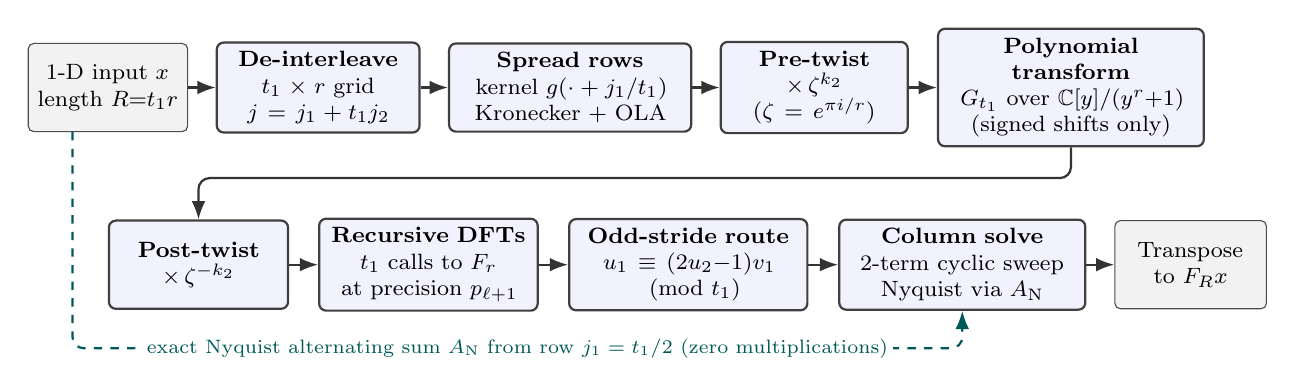
\begin{tikzpicture}[
  font=\footnotesize,
  >=Latex,
  box/.style={draw=black!75, fill=blue!5!white, thick, rounded corners=2.5pt, minimum height=1.12cm, align=center, inner sep=3.2pt},
  iobox/.style={draw=black!70, fill=black!5, rounded corners=2pt, minimum height=1.12cm, align=center, inner sep=3.2pt},
  arr/.style={->, thick, draw=black!80}
]
  % Top row: left to right
  \node[iobox, text width=1.80cm] (in) at (0.95, 1.35)
    {1-D input $x$\\length $R{=}t_1 r$};
  \node[box, text width=2.35cm] (grid) at (3.62, 1.35)
    {\textbf{De-interleave}\\$t_1 \times r$ grid\\$j = j_1 + t_1 j_2$};
  \node[box, text width=2.85cm] (spread) at (6.82, 1.35)
    {\textbf{Spread rows}\\kernel $g(\cdot + j_1/t_1)$\\Kronecker + OLA};
  \node[box, text width=2.15cm] (pre) at (9.92, 1.35)
    {\textbf{Pre-twist}\\$\times\,\zeta^{k_2}$\\($\zeta = e^{\pi i/r}$)};
  \node[box, text width=3.15cm] (poly) at (13.18, 1.35)
    {\textbf{Polynomial transform}\\$G_{t_1}$ over $\C[y]/(y^r{+}1)$\\(signed shifts only)};

  \draw[arr] (in) -- (grid);
  \draw[arr] (grid) -- (spread);
  \draw[arr] (spread) -- (pre);
  \draw[arr] (pre) -- (poly);

  % Bottom row: shifted right of x = 0.96 so the Nyquist corridor at x = 0.50 clears every box
  \node[box, text width=2.05cm] (post) at (2.10, -0.90)
    {\textbf{Post-twist}\\$\times\,\zeta^{-k_2}$};
  \node[box, text width=2.55cm] (rec) at (5.02, -0.90)
    {\textbf{Recursive DFTs}\\$t_1$ calls to $F_r$\\at precision $p_{\ell+1}$};
  \node[box, text width=2.80cm] (route) at (8.32, -0.90)
    {\textbf{Odd-stride route}\\$u_1 \equiv (2u_2{-}1)v_1$\\$\pmod{t_1}$};
  \node[box, text width=2.90cm] (deconv) at (11.80, -0.90)
    {\textbf{Column solve}\\2-term cyclic sweep\\Nyquist via $A_{\mathrm{N}}$};
  \node[iobox, text width=1.70cm] (out) at (14.70, -0.90)
    {Transpose\\to $F_R x$};

  % Connecting arrow from top-right to bottom-left via clean middle corridor
  \draw[arr, rounded corners=4pt] (poly.south) -- (13.18, 0.20) -- (2.10, 0.20) -- (post.north);

  \draw[arr] (post) -- (rec);
  \draw[arr] (rec) -- (route);
  \draw[arr] (route) -- (deconv);
  \draw[arr] (deconv) -- (out);

  % Nyquist side path from bottom border of 1-D input along open left/bottom corridor to Column solve
  \draw[->, thick, dashed, teal!70!black, rounded corners=4pt]
    ([xshift=-0.45cm]in.south) |- (6.15, -1.96) -| (deconv.south);
  \node[fill=white, inner sep=1.8pt, font=\scriptsize, text=teal!70!black] at (6.15, -1.96)
    {exact Nyquist alternating sum $A_{\mathrm{N}}$ from row $j_1 = t_1/2$ (zero multiplications)};
\end{tikzpicture}%
}
\caption{One recursive level of \texttt{FastDFT} on a single $t_1 \times r$ power-of-two grid ($R = t_1 r$). Row spreading turns Cooley--Tukey twiddles into a two-alias column mixture. The Nussbaumer--Quandalle polynomial transform over $\C[y]/(y^r + 1)$ and $t_1$ recursive length-$r$ transforms evaluate $F_{t_1, r}$ without butterfly multiplications, and per-column two-term and Nyquist solvers recover $F_R x$.}
\label{fig:pipeline}
\end{figure}

Figure~\ref{fig:pipeline} shows the resulting single-level pipeline. Unlike~\cite{HvdH21}, which embeds into pairwise coprime lengths by Chinese remaindering and resamples between grids of different sizes, the input, spread array, and output here occupy one $t_1 \times r$ power-of-two grid with no prime lengths and no grid expansion. Unlike general NUFFT gridding~\cite{DR93,PST01,GL04,BMK19}, where arbitrary sample nodes require point-by-point interpolation onto an oversampled grid followed by diagonal division by $\hat{g}$, the shift $j_1 / t_1$ here is constant along each row, so spreading is a shift-invariant cyclic convolution of length $r$ and oversampling is replaced by a two-term cyclic solve per column.

\subsection{Computing \texorpdfstring{$F_{t_1, r}$}{F\_\{t1, r\}} without multiplications}\label{sec:overview-poly}

Evaluating $F_{t_1, r} U$ directly by row and column FFTs would still perform $\Theta(R \log t_1)$ complex butterfly multiplications along the first axis. Instead, we use the polynomial-transform reduction of Nussbaumer and Quandalle~\cite{NQ79,Nussbaumer80,Nussbaumer82} with negacyclic weighting~\cite{SS71,CF94} (Proposition~\ref{thm:twisted}). Because $r$ is a power of two, the quotient ring $\Rr_r = \C[y]/(y^r + 1)$ contains the synthetic root $y$ of order $2r$ ($y^r \equiv -1$). Since $t_1 \mid r$ with $\nu = r / t_1 \in \{1, 2\}$, the monomial $\omega_{t_1} := y^{2\nu}$ satisfies $\omega_{t_1}^{t_1/2} = y^r \equiv -1$ and has exact order $t_1$ in $\Rr_r$. The length-$t_1$ polynomial transform
\[
  (G_{t_1} P)_{v_1}(y) := \frac{1}{t_1}\sum_{j_1=0}^{t_1-1} P_{j_1}(y)\, y^{2\nu j_1 v_1} \pmod{y^r + 1}
\]
can therefore be computed by $\log_2 t_1$ radix-2 butterfly stages over $\Rr_r$ using only additions, halvings, and signed cyclic shifts of $r$-coefficient polynomials, with zero scalar multiplications (Lemma~\ref{lem:syn-fft}).

To connect $\Rr_r$ to the column transforms of $F_{t_1, r}$, let $\zeta = e^{\pi i / r}$ ($\zeta^r = -1$). The $r$ roots of $y^r + 1 = 0$ are the odd powers $\zeta^{2u_2 - 1}$ for $u_2 \in \{0, \dots, r-1\}$, giving $r$ ring homomorphisms $\phi_{u_2}\colon \Rr_r \to \C$, $y \mapsto \zeta^{2u_2 - 1}$. Pre-twisting column $k_2$ of row $j_1$ by $\zeta^{k_2}$ forms $P_{j_1}(y) = \sum_{k_2=0}^{r-1} \zeta^{k_2} U_{j_1, k_2} y^{k_2}$, whose image $\phi_{u_2}(P_{j_1}) = \sum_{k_2=0}^{r-1} U_{j_1, k_2} e^{2\pi i k_2 u_2 / r}$ is the unnormalized length-$r$ DFT along row $j_1$. Conversely, for each output polynomial $Q_{v_1} = (G_{t_1} P)_{v_1}$, post-twisting coefficient $k_2$ by $\zeta^{-k_2}$ and applying a recursive length-$r$ transform $F_r$ evaluates $\frac{1}{r}\phi_{u_2}(Q_{v_1})$ across all $u_2$ simultaneously. Finally, $\phi_{u_2}(y^{2\nu j_1 v_1}) = e^{2\pi i j_1 (2u_2 - 1) v_1 / t_1}$, and because $2u_2 - 1$ is odd while $t_1$ is a power of two, $v_1 \mapsto u_1 := (2u_2 - 1) v_1 \bmod t_1$ permutes $\{0, \dots, t_1 - 1\}$ bijectively in every column $u_2$. This multiplication-free polynomial transform, together with the per-level tape transposes and odd-stride routing, is the only $\Theta(n \log n)$ work term in the entire algorithm.

\subsection{The kernel and two-term deconvolution}\label{sec:overview-kernel}

The choice of spreading kernel $g$ governs how precision grows with recursion depth. Suppose first that one spreads with a plain Gaussian $g_{\mathrm{plain}}(t) = e^{-\pi t^2 / \alpha_{\mathrm{plain}}^2}$ scaled by $\pi \alpha_{\mathrm{plain}}^2 = p_{\mathrm{work},\ell} \ln 2$ so that excluded aliases decay to $O(2^{-p_{\mathrm{work},\ell}})$. Its Fourier transform $\widehat{g_{\mathrm{plain}}}(\xi) = \alpha_{\mathrm{plain}} 2^{-p_{\mathrm{work},\ell} \xi^2}$ peaks at $\xi = 0$ but falls at the Nyquist boundary $\xi = 1/2$ ($u_2 = r/2$) to $\alpha_{\mathrm{plain}} 2^{-p_{\mathrm{work},\ell}/4}$ (Figure~\ref{fig:kernel}(a)). Inverting the column system at $u_2 \approx r/2$ then divides by $O(2^{-p_{\mathrm{work},\ell}/4})$; in the natural analysis (a heuristic estimate, not used elsewhere) this loses about $\tfrac{1}{4} p_{\mathrm{work},\ell}$ bits of accuracy at every level and leads to a multiplicative precision schedule ($p_{\ell+1} \gtrsim \tfrac{5}{4} p_{\mathrm{work},\ell}$) instead of an additive one.

We eliminate this Nyquist attenuation by multiplying the Gaussian by $\sinc(t) = \frac{\sin(\pi t)}{\pi t}$, obtaining the windowed sinc-Gaussian kernel (Theorem~\ref{thm:poisson})
\begin{equation}\label{eq:overview-kernel}
  g(t) := \sinc(t)\, e^{-\pi t^2 / \alpha^2}, \qquad \alpha := 2\sqrt{\frac{p_{\mathrm{work},\ell}\ln 2}{\pi}}.
\end{equation}
In frequency space, multiplying by $\sinc(t)$ convolves the Gaussian $\alpha e^{-\pi \alpha^2 \xi^2}$ with the unit box $\mathbf{1}_{[-1/2, 1/2]}$, yielding the erf-smoothed boxcar
\[
  \hat{g}(\xi) = \frac{1}{2}\left[\erf\!\left(\sqrt{\pi}\alpha\!\left(\xi + \frac{1}{2}\right)\right) - \erf\!\left(\sqrt{\pi}\alpha\!\left(\xi - \frac{1}{2}\right)\right)\right].
\]
Because the shifted intervals $[y - m - 1/2, y - m + 1/2]$ tile $\R$, the weights satisfy the exact partition of unity $\sum_{m \in \Z} \hat{g}(y - m) = 1$. For every $y = u_2 / r \in [0, 1)$, the two retained weights $c_0(u_2) = \hat{g}(y)$ and $c_1(u_2) = \hat{g}(y - 1) = \hat{g}(1 - y)$ satisfy $\max(c_0, c_1) \ge \hat{g}(1/2) = \frac{1}{2}\erf(\sqrt{\pi}\alpha) > 0.49999999$ (for $p_{\mathrm{work},\ell} \ge 8$), while all omitted aliases $m \notin \{0, 1\}$ telescope in closed form to $1 - c_0(u_2) - c_1(u_2) < 0.120 \cdot 2^{-p_{\mathrm{work},\ell}}$ (Theorem~\ref{thm:deconv}(1)).

\begin{figure}[t]
\centering
\resizebox{0.98\textwidth}{!}{%
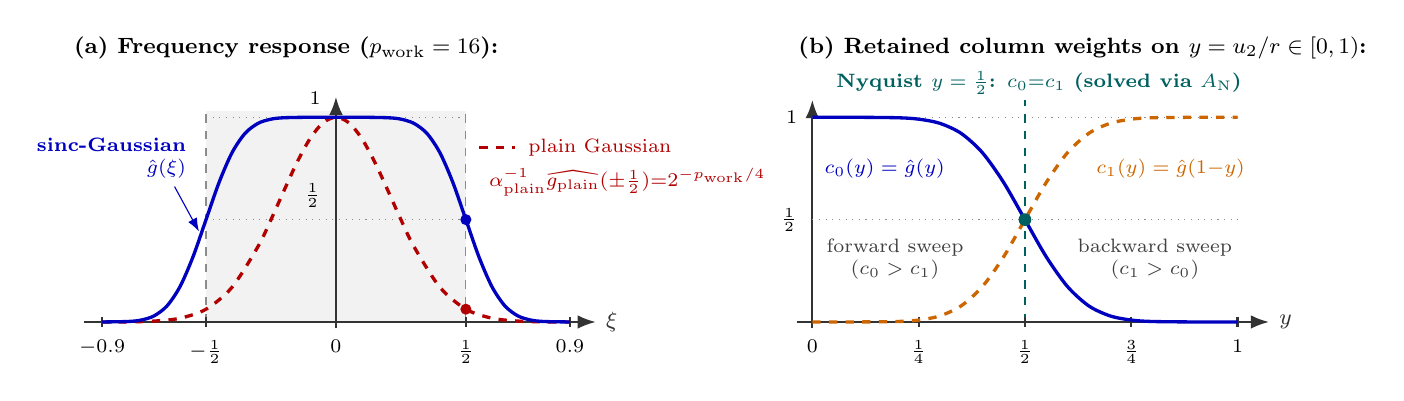
\begin{tikzpicture}[font=\footnotesize, >=Latex]
  % ---------------- Panel (a): Passband comparison ----------------
  \begin{scope}[xshift=0cm]
    \node[anchor=west, font=\footnotesize\bfseries] at (-3.45, 3.48)
      {(a) Frequency response ($p_{\mathrm{work}} = 16$):};

    % Axes: x from -0.95 to 0.95 scaled by 3.3 -> [-3.135, 3.135]; y scaled by 2.6
    \fill[black!5] (-1.65, 0) rectangle (1.65, 2.68);
    \draw[->, thick, black!80] (-3.20, 0) -- (3.30, 0) node[right] {$\xi$};
    \draw[->, thick, black!80] (0, -0.08) -- (0, 2.86);
    \draw[dotted, black!45] (-1.65, 2.60) -- (1.65, 2.60);
    \draw[dotted, black!45] (-1.65, 1.30) -- (1.65, 1.30);
    \draw[dashed, black!45] (-1.65, 0) -- (-1.65, 2.68);
    \draw[dashed, black!45] (1.65, 0) -- (1.65, 2.68);

    \node[above left=1pt and 2pt, font=\scriptsize] at (0, 2.60) {$1$};
    \node[above left=1pt and 2pt, font=\scriptsize] at (0, 1.30) {$\tfrac{1}{2}$};
    \foreach \x/\xlab in {-2.97/-0.9, -1.65/-\tfrac{1}{2}, 0/0, 1.65/\tfrac{1}{2}, 2.97/0.9} {
      \draw[thick, black!80] (\x, -0.06) -- (\x, 0.06);
      \node[below=2pt, font=\scriptsize] at (\x, -0.04) {$\xlab$};
    }

    % Plain Gaussian normalized: 2^{-16 \xi^2} (x = 3.3*\xi, y = 2.6*val)
    \draw[very thick, red!70!black, dashed] plot[smooth] coordinates {
      (-2.970,0.0003) (-2.640,0.0021) (-2.310,0.0114) (-1.980,0.0481) (-1.650,0.1625)
      (-1.320,0.4410) (-0.990,0.9584) (-0.825,1.3000) (-0.660,1.6684) (-0.495,2.0259)
      (-0.330,2.3270) (-0.165,2.5290) (0.000,2.6000) (0.165,2.5290) (0.330,2.3270)
      (0.495,2.0259) (0.660,1.6684) (0.825,1.3000) (0.990,0.9584) (1.320,0.4410)
      (1.650,0.1625) (1.980,0.0481) (2.310,0.0114) (2.640,0.0021) (2.970,0.0003)
    };

    % Windowed sinc-Gaussian \hat{g}(\xi) at p_work = 16
    \draw[very thick, blue!75!black] plot[smooth] coordinates {
      (-2.970,0.0003) (-2.640,0.0062) (-2.475,0.0242) (-2.310,0.0775) (-2.145,0.2049)
      (-1.980,0.4501) (-1.815,0.8289) (-1.650,1.3000) (-1.485,1.7711) (-1.320,2.1499)
      (-1.155,2.3951) (-0.990,2.5225) (-0.825,2.5758) (-0.660,2.5938) (-0.330,2.6000)
      (0.000,2.6000) (0.330,2.6000) (0.660,2.5938) (0.825,2.5758) (0.990,2.5225)
      (1.155,2.3951) (1.320,2.1499) (1.485,1.7711) (1.650,1.3000) (1.815,0.8289)
      (1.980,0.4501) (2.145,0.2049) (2.310,0.0775) (2.475,0.0242) (2.640,0.0062)
      (2.970,0.0003)
    };

    \fill[blue!75!black] (1.650, 1.3000) circle (2.0pt);
    \fill[red!70!black] (1.650, 0.1625) circle (2.0pt);

    % Left callout in open region x < -1.78, y in [1.75, 2.40]
    \node[blue!75!black, font=\scriptsize\bfseries, align=right, anchor=east] at (-1.78, 2.08)
      {sinc-Gaussian\\$\hat{g}(\xi)$};
    \draw[->, thin, blue!75!black] (-2.05, 1.72) -- (-1.74, 1.15);

    % Right callout/legend in open region x > 1.80, y in [1.55, 2.40]
    \draw[very thick, red!70!black, dashed] (1.82, 2.22) -- (2.28, 2.22);
    \node[red!70!black, font=\scriptsize, align=left, anchor=west] at (2.32, 2.22)
      {plain Gaussian};
    \node[red!70!black, font=\scriptsize, align=left, anchor=west] at (1.82, 1.78)
      {$\alpha_{\mathrm{plain}}^{-1}\widehat{g_{\mathrm{plain}}}(\pm\tfrac{1}{2}){=}2^{-p_{\mathrm{work}}/4}$};
  \end{scope}

  % ---------------- Panel (b): Column weights c_0(y), c_1(y) ----------------
  \begin{scope}[xshift=6.05cm]
    \node[anchor=west, font=\footnotesize\bfseries] at (-0.30, 3.48)
      {(b) Retained column weights on $y = u_2 / r \in [0, 1)$:};

    % Axes: y in [0, 1] scaled by 5.4 -> [0, 5.4]; vertical scaled by 2.6
    \draw[->, thick, black!80] (-0.20, 0) -- (5.80, 0) node[right] {$y$};
    \draw[->, thick, black!80] (0, -0.08) -- (0, 2.82);
    \draw[dotted, black!45] (0, 2.60) -- (5.40, 2.60);
    \draw[dotted, black!45] (0, 1.30) -- (5.40, 1.30);
    \draw[dashed, teal!75!black, thick] (2.70, 0) -- (2.70, 2.82);

    \node[left=2pt, font=\scriptsize] at (0, 2.60) {$1$};
    \node[left=2pt, font=\scriptsize] at (0, 1.30) {$\tfrac{1}{2}$};
    \foreach \x/\xlab in {0/0, 1.35/\tfrac{1}{4}, 2.70/\tfrac{1}{2}, 4.05/\tfrac{3}{4}, 5.40/1} {
      \draw[thick, black!80] (\x, -0.06) -- (\x, 0.06);
      \node[below=2pt, font=\scriptsize] at (\x, -0.04) {$\xlab$};
    }

    % c_0(y) = \hat{g}(y) (x = 5.4*y, y_coord = 2.6*val)
    \draw[very thick, blue!75!black] plot[smooth] coordinates {
      (0.000,2.6000) (0.540,2.5997) (1.080,2.5938) (1.350,2.5758) (1.620,2.5225)
      (1.890,2.3951) (2.160,2.1499) (2.430,1.7711) (2.700,1.3000) (2.970,0.8289)
      (3.240,0.4501) (3.510,0.2049) (3.780,0.0775) (4.050,0.0242) (4.320,0.0062)
      (4.860,0.0003) (5.400,0.0000)
    };

    % c_1(y) = \hat{g}(1 - y)
    \draw[very thick, orange!80!black, dashed] plot[smooth] coordinates {
      (0.000,0.0000) (0.540,0.0003) (1.080,0.0062) (1.350,0.0242) (1.620,0.0775)
      (1.890,0.2049) (2.160,0.4501) (2.430,0.8289) (2.700,1.3000) (2.970,1.7711)
      (3.240,2.1499) (3.510,2.3951) (3.780,2.5225) (4.050,2.5758) (4.320,2.5938)
      (4.860,2.5997) (5.400,2.6000)
    };

    \fill[teal!75!black] (2.700, 1.3000) circle (2.3pt);

    \node[blue!75!black, font=\scriptsize\bfseries] at (0.92, 1.95) {$c_0(y) = \hat{g}(y)$};
    \node[orange!80!black, font=\scriptsize\bfseries] at (4.55, 1.95) {$c_1(y) = \hat{g}(1{-}y)$};
    \node[font=\scriptsize, text=black!75, align=center] at (1.05, 0.80)
      {forward sweep\\($c_0 > c_1$)};
    \node[font=\scriptsize, text=black!75, align=center] at (4.35, 0.80)
      {backward sweep\\($c_1 > c_0$)};
    \node[teal!75!black, font=\scriptsize\bfseries] at (2.88, 3.04)
      {Nyquist $y=\tfrac{1}{2}$: $c_0{=}c_1$ (solved via $A_{\mathrm{N}}$)};
  \end{scope}
\end{tikzpicture}%
}
\caption{Passband behavior and two-term deconvolution weights. (a)~At $\xi = \pm 1/2$, the normalized plain Gaussian drops to $2^{-p_{\mathrm{work}}/4}$, whereas the windowed sinc-Gaussian kernel maintains $\hat{g}(\pm 1/2) \approx 1/2$. (b)~Along each column $y = u_2 / r \in [0, 1)$, the retained weights $c_0(y)$ and $c_1(y)$ cross only at the Nyquist column $y = 1/2$; non-Nyquist columns have $\|B^{-1}\|_{\infty \to \infty} = 1/|c_0 - c_1| < 2.36\, t_1$, and $y = 1/2$ is closed by the exact input alternating sum $A_{\mathrm{N}}$.}
\label{fig:kernel}
\end{figure}

Figure~\ref{fig:kernel}(b) illustrates how each column $u_2 \in \{0, \dots, r-1\}$ is deconvolved to recover $Z_{u_1} = (F_R x)_{u_2 + r u_1}$ from $Y_{u_1} \approx c_0(u_2) Z_{u_1} + c_1(u_2) Z_{(u_1 - 1)\bmod t_1}$. Whenever $u_2 \ne r/2$, $|1/2 - y| \ge 1/r \ge 1/(2 t_1)$ separates $c_0$ and $c_1$ enough that the damping power $a^{t_1} = (\min(c_0, c_1)/\max(c_0, c_1))^{t_1}$ is strictly below $0.14$ (Theorem~\ref{thm:deconv}(2)). Sweeping forward when $u_2 < r/2$ ($c_0 > c_1$) or backward when $u_2 > r/2$ ($c_1 > c_0$) inverts the cyclic bidiagonal operator $B$ in $O(t_1)$ scalar operations with $\ell_\infty$ inverse norm $1 / |c_0(u_2) - c_1(u_2)| < 2.36\, t_1$.

At the single Nyquist column $u_2 = r/2$ ($y = 1/2$), symmetry gives $c_0(r/2) = c_1(r/2) = c \approx 1/2$. Because $t_1 \ge 2$ is even, the cyclic equations $c(Z_{u_1} + Z_{(u_1 - 1)\bmod t_1}) = Y_{u_1}$ sum with alternating signs $(-1)^{u_1}$ to zero and leave the alternating mode $\sum_{u_1=0}^{t_1-1} (-1)^{u_1} Z_{u_1}$ undetermined. By character orthogonality on $\Z_{t_1}$, however, that alternating sum collapses directly in the spatial domain to a single row of the input vector (Theorem~\ref{thm:deconv}(3), equation~\eqref{eq:nyquist-id}):
\[
  A_{\mathrm{N}} := \sum_{u_1=0}^{t_1-1} (-1)^{u_1} Z_{u_1}
  = \frac{i}{r}\sum_{j_2=0}^{r-1} (-1)^{j_2} x\!\left(\frac{t_1}{2} + t_1 j_2\right).
\]
Accumulating $A_{\mathrm{N}}$ from row $j_1 = t_1 / 2$ before spreading uses only additions, subtractions, and a power-of-two shift by $r^{-1}$, with zero scalar multiplications, and closes the open bidiagonal chain at $u_2 = r/2$ with inverse norm below $1.0000001\, t_1 < 2.36\, t_1$.

\subsection{Additive precision schedule}\label{sec:overview-precision}

Uniform $O(t_1)$ conditioning across all $r$ columns yields a purely additive precision recurrence along the recursion tree (Lemma~\ref{lem:forward}). At depth $\ell$, a node of length $R_\ell = 2^{K_\ell} = t_{1,\ell} r_\ell$ receives an input $x \in \Cg_{p_\ell+2}^{R_\ell}$ and must approximate $F_{R_\ell} x$ within $\ell_\infty$ error $2^{-p_\ell} \max(1, \|x\|_\infty)$. Two error groups enter before final quantization to $\Cg_{p_\ell+2}$:
\begin{enumerate}[label=(\arabic*),leftmargin=*,nosep,topsep=3pt]
  \item \emph{Excluded Poisson aliases:} Dropping modes $m \notin \{0, 1\}$ perturbs the ideal column right-hand side by at most $0.120 \cdot 2^{-p_{\mathrm{work},\ell}} \max(1, \|x\|_\infty)$, which multiplication by $B^{-1}$ ($\|B^{-1}\|_{\infty \to \infty} < 2.36\, t_{1,\ell}$) amplifies to at most $\frac{1}{2} t_{1,\ell} 2^{-p_{\mathrm{work},\ell}} \max(1, \|x\|_\infty)$.
  \item \emph{Spreading, polynomial transform, recursive calls, and column solvers.} Spatial window truncation and tap quantization in Step~1, rounding in the twists and $\log_2 t_{1,\ell}$ polynomial-transform stages of Steps~2a--2c, and the inductive error $2^{-p_{\ell+1}}$ of the $t_{1,\ell}$ child calls in Step~2d (on inputs of norm $O(r_\ell \max(1, \|x\|_\infty))$) perturb the column right-hand sides by $O(r_\ell 2^{-p_{\ell+1}} \max(1, \|x\|_\infty))$. Together with fixed-point rounding across the $O(t_{1,\ell})$-step column sweeps of Step~3, these terms sum after deconvolution to at most $200 R_\ell 2^{-p_{\ell+1}} \max(1, \|x\|_\infty)$.
\end{enumerate}
Choosing the additive precision schedule~\eqref{eq:cert-sched},
\[
  p_{\mathrm{work},\ell} := p_\ell + K_\ell + 6, \qquad
  p_{\ell+1} := p_{\mathrm{work},\ell} + K_\ell + 6 = p_\ell + 2 K_\ell + 12,
\]
makes $\frac{1}{2} t_{1,\ell} 2^{-p_{\mathrm{work},\ell}} \le 2^{-p_\ell - 7}$ and $200 R_\ell 2^{-p_{\ell+1}} \le \frac{25}{2048} 2^{-p_\ell}$. Adding the final $\Cg_{p_\ell+2}$ rounding error $\frac{\sqrt{2}}{8} 2^{-p_\ell}$ gives a total error below $0.197 \cdot 2^{-p_\ell} \max(1, \|x\|_\infty) < \frac{1}{4} 2^{-p_\ell} \max(1, \|x\|_\infty)$, closing the induction at every non-leaf node (and leaves $R_L \le 4 p_L^2$ close at precision $q_b = p_L + K_L + 4$).

Because $K_{\ell+1} = \lceil K_\ell / 2 \rceil$, the log-length halves at each level and hits the leaf threshold $R_L \le 4 p_L^2$ in $L = O(\log K_0) = O(\log \log n)$ levels. Summing $2 K_j + 12$ from $0$ to $\ell - 1$ bounds the precision at every level by $p_\ell \le p_0 + 4 K_0 + 14 \ell = \Theta(\log n)$, while the integer scalar height $H_\ell$ satisfies $H_\ell \le 1 + K_0 + 2\ell = O(\log n)$ (Section~\ref{sec:prelim}). Every level therefore stores $R_0$ fixed-width complex records of $w_\ell = \Theta(\log n)$ bits, maintaining the invariant bit volume $R_0 p_\ell = \Theta(n)$ throughout the recursion.

\subsection{Cost on a multitape Turing machine}\label{sec:overview-cost}

With $R_0$ active entries of $\Theta(\log n)$ bits at every depth $\ell < L$, the multitape Turing machine cost breaks cleanly into one $\Theta(n \log n)$ movement-and-shift term and $o(n \log n)$ arithmetic and table work (Section~\ref{sec:main-proof}):
\begin{itemize}[leftmargin=*,nosep,topsep=3pt]
  \item \emph{Polynomial transform and tape routing:} At depth $\ell$, each of the $R_0 / R_\ell$ nodes performs $\log_2 t_{1,\ell} = \lfloor K_\ell / 2 \rfloor$ radix-2 polynomial-transform stages over $\Rr_{r_\ell}$ (Lemma~\ref{lem:syn-fft}), two matrix transposes, and one odd-stride merge-sort column permutation $u_1 = (2u_2 - 1) v_1 \bmod t_{1,\ell}$ (Lemma~\ref{lem:routing}), costing $O\bigl(R_\ell p_{\ell+1}(1 + \log_2 t_{1,\ell})\bigr)$ steps per node. Across all $R_0 / R_\ell$ nodes, this is $O\bigl(n(1 + K_0 / 2^{\ell+1})\bigr)$ steps at depth $\ell$, which sums geometrically over $\ell = 0, \dots, L - 1$ to $O(n K_0 + n L) = O(n \log n)$.
  \item \emph{Kronecker spreading and window cancellation:} Truncating $g(d + j_1 / t_{1,\ell})$ at radius $m_{1,\ell} = \Theta(p_{\ell+1})$ and folding modulo $r_\ell$ gives a filter of effective length $\tilde{W}_\ell = \min(2m_{1,\ell} + 1, r_\ell)$. Using overlap-add of block size $\tilde{W}_\ell$ and signed two's-complement Kronecker substitution~\cite{Schonhage82,Harvey09} at slot width $B_{\mathrm{slot}} = \Theta(p_{\ell+1})$ reduces row spreading across a node to $O(R_\ell / \tilde{W}_\ell)$ integer products of bit-length $\Theta(\tilde{W}_\ell p_{\ell+1}) = O((\log n)^2)$ (Theorem~\ref{thm:spread}). The window length $\tilde{W}_\ell$ cancels between the block count and the packed bit-length, so all multiplications in spreading, scalar twists, column sweeps, and leaf FFTs ($R_L \le 4 p_L^2$) operate on $O((\log n)^2)$-bit integers, of total bit volume $O(n)$ per level for $\ell < L$ and $O(n \log\log n)$ at the leaf level (its $K_L = O(\log\log n)$ butterfly stages; Part~3(c) of the proof of Theorem~\ref{thm:main}).
  \item \emph{Tables and non-circular bootstrap:} All shared per-level filter, twist, solver, and leaf-twiddle tables are evaluated from truncated Taylor and Machin series at guard precision in time $O(\sqrt{n}(\log n)^{7/2}\allowbreak\log\log n) = o(n)$ (equation~\eqref{eq:table-precomp}), and a breadth-first ping-pong schedule executes the recursion on $O(1)$ tapes (Appendix~\ref{app:elementary}). To avoid circularity in the asymptotic constant when multiplying $O((\log n)^2)$-bit integers on $O(1)$ tapes, the proof in Section~\ref{sec:main-proof} uses a fixed three-stage bootstrap. A base radix-2 FFT multiplier with schoolbook twiddles running in $O(N(\log 2N)^2)$ steps feeds a first recursive multiplier running in $O(N \log 2N)$ steps, which in turn multiplies all inner operands of the outer call in $O\bigl(n(\log\log n)^2\bigr)$ total steps.
\end{itemize}

\subsection{What is verified and what is executed}\label{sec:overview-verified}

Section~\ref{sec:lean} describes the Lean~4 formalization~\cite{LeanMS26} of Theorem~\ref{thm:lean}, which constructs a single parameter-free eight-stack binary machine \texttt{tmIntMul} (which an eight-tape Turing machine simulates with constant-factor slowdown, one tape per stack; this standard simulation is not part of the formal development). From Lean's three standard logical axioms, it proves that \texttt{tmIntMul} halts with the exact $2n$-bit product within $C \cdot n \lfloor \log_2 n \rfloor$ steps and $O(n \log n)$ elementary stack operations for all $n \ge 2$. The analytic and fixed-point bounds on which the formal proof rests are proved inside the same library (Table~\ref{tab:lean-map}). Section~\ref{sec:empirical} reports the C/GMP measurements~\cite{CGMP26}: bit-exact agreement with GMP at every tested size up to $10^9$ bits, at $153$--$323$ times the single-threaded running time of \texttt{mpz\_mul}.

\section{Preliminaries}\label{sec:prelim}

This section fixes global notation (Section~\ref{sec:notation}), defines the multitape Turing machine model and dyadic fixed-point grids (Section~\ref{sec:prelim-model}), states the elementary-function table contract and tape schedule (Section~\ref{sec:tables}), records the matrix transposition and odd-stride routing bounds (Section~\ref{sec:routing}), and recalls our Discrete Fourier Transform and polynomial-transform conventions (Section~\ref{sec:prelim-dft}).

\subsection{Notation}\label{sec:notation}

Logarithms are natural ($\ln$) unless a base is written ($\log_2$). For an integer $R \ge 1$, a vector $x = (x_0, \dots, x_{R-1}) \in \C^R$ carries the Euclidean supremum norm $\|x\|_\infty := \max_{0 \le j < R} |x_j|$, where $|a + i b| = \sqrt{a^2 + b^2}$ is the complex modulus, as well as the coordinatewise supremum norm $\|x\|_{\infty,\mathrm{coord}} := \max_{0 \le j < R} \max(|\operatorname{Re}(x_j)|, |\operatorname{Im}(x_j)|)$. For a linear map $B\colon \C^m \to \C^m$, $\|B\|_{\infty \to \infty}$ denotes the induced $\ell_\infty$ operator norm (the maximum absolute row sum). Table~\ref{tab:notation} summarizes the notation used throughout the paper.

\subsection{Multitape Turing machine and fixed-point grids}\label{sec:prelim-model}

Following Sch\"onhage and Strassen~\cite{SS71} and Harvey and van der Hoeven~\cite[Section~2.1]{HvdH21}, our model of computation is a deterministic multitape Turing machine with a fixed finite alphabet and a fixed finite number of tapes (all complexity bounds hold \emph{a fortiori} on the standard $\Theta(\log n)$-bit Word RAM). Throughout the paper, a ``bit operation'' means a single Turing machine step (one state transition, tape-symbol read/write, and $\{-1, 0, +1\}$ head move on each of the $O(1)$ tapes), so all sequential tape scans, head movements, rewinds, and counter updates are charged explicitly. The input to a multiplication of two $n$-bit integers $A, B$ is the concatenation of their fixed-width $n$-bit binary strings ($2n$ bits, so $n$ is determined by the input) on a designated input tape, and the output is the fixed-width $2n$-bit binary string of $A \cdot B$ on a designated output tape; both are among the $O(1)$ tapes.

\begin{definition}[Fixed-point grids and rounding]\label{def:grid}
For an integer $q \ge 0$, define the dyadic fixed-point real and complex grids
\[
  \Rg_q := \bigl\{2^{-q} a : a \in \Z\bigr\}, \qquad \Cg_q := \bigl\{2^{-q}(a + i b) : a, b \in \Z\bigr\}.
\]
Here $q$ counts fractional bits after the binary point, while the integer part is represented in signed two's-complement binary without modular wrap-around. A target accuracy parameter $p \in \Z_{\ge 1}$ uses the working grid $\Cg_{p+2}$ ($q = p + 2$). For $x \in \R$, let $\Quant_q(x) := 2^{-q}\operatorname{round}(2^q x) \in \Rg_q$ denote nearest-grid rounding under any fixed deterministic tie-breaking rule on half-integers (such as ties to even, or $\lfloor 2^q x + 1/2 \rfloor$), and for $z = x + i y \in \C$, define coordinatewise rounding $\Quant_q(z) := \Quant_q(x) + i \Quant_q(y) \in \Cg_q$.
\end{definition}

\begin{table}[!ht]
\centering
\footnotesize
\renewcommand{\arraystretch}{0.96}
\caption{Summary of notation used throughout Sections~\ref{sec:prelim}--\ref{sec:main-proof} and Appendices~\ref{app:elementary}--\ref{app:deferred}.}\label{tab:notation}
\begin{tabular}{@{}>{\raggedright}p{0.28\textwidth}>{\raggedright\arraybackslash}p{0.67\textwidth}@{}}
\toprule
Symbol & Meaning \\
\midrule
$n,\ b,\ N$ & bit length of input integers $A, B \ge 0$, radix-$2^b$ chunk width $b = \max(4, \lfloor \log_2 n \rfloor)$, and chunk count $N = \lceil n / b \rceil$ \\
$R_0 = 2^{K_0},\ p_0$ & root transform length ($2N \le R_0 < 4N$) with $K_0 = \log_2 R_0$, and root target precision $p_0 = 2b + 2K_0 + 6$ \\
$R_\ell = 2^{K_\ell} = t_{1,\ell} r_\ell$ & transform length at recursion depth $\ell$, with $K_\ell = \log_2 R_\ell$, $t_{1,\ell} = 2^{\lfloor K_\ell / 2 \rfloor}$, $r_\ell = 2^{\lceil K_\ell / 2 \rceil}$, and $\nu_\ell = r_\ell / t_{1,\ell} \in \{1, 2\}$ \\
$k_{1,\ell},\ k_{2,\ell}$ & $\log_2 t_{1,\ell}$ and $\log_2 r_\ell$ ($k_{1,\ell} + k_{2,\ell} = K_\ell$) \\
$L$ & leaf recursion depth (first depth $\ell$ where $R_\ell \le 4 p_\ell^2$) \\
$p_\ell,\ p_{\mathrm{work},\ell},\ p_{\ell+1}$ & target precision at depth $\ell$, working cutoff $p_{\mathrm{work},\ell} = p_\ell + K_\ell + 6$, and child target precision $p_{\ell+1} = p_\ell + 2K_\ell + 12$ \\
$\Rg_q,\ \Cg_q,\ \Quant_q$ & real and complex dyadic grids $2^{-q}\Z$ and $2^{-q}(\Z + i\Z)$ ($q = p + 2$ for target precision $p$), and coordinatewise nearest-grid rounding \\
$q_{\mathrm{child}},\ u = 2^{-p_{\ell+1}}$ & child fractional grid parameter $q_{\mathrm{child}} = p_{\ell+1} + 2$ and unit accuracy scale of child calls (the letter $u$ also denotes the one-dimensional frequency index $u = u_2 + r u_1$ of~\eqref{eq:dft-1d}; the meaning is fixed by context: $u_2$ indexes columns, $u = 2^{-p_{\ell+1}}$ is the accuracy scale) \\
$H_\ell,\ w_{\mathrm{coord},\ell},\ w_\ell$ & integer coordinate height bound at depth $\ell$, signed coordinate bit width, and complex record width $w_\ell = 2 w_{\mathrm{coord},\ell}$ \\
$\Rr_r = \C[y]/(y^r + 1),\ G_{t_1}$ & negacyclic polynomial ring of rank $r$ and normalized length-$t_1$ polynomial transform over $\Rr_r$ \\
$P_{j_1}(y),\ Q_{v_1}(y)$ & input and output polynomials in $\Rr_r$ of the polynomial transform $G_{t_1}$ \\
$F_R,\ F_{t_1, r}$ & normalized positive one-dimensional DFT of length $R$ and two-dimensional DFT of shape $t_1 \times r$ \\
$g(t),\ \hat{g}(\xi),\ \alpha_\ell$ & windowed sinc-Gaussian kernel $\sinc(t)e^{-\pi t^2 / \alpha_\ell^2}$, its continuous Fourier transform, and $\alpha_\ell = 2\sqrt{p_{\mathrm{work},\ell}\ln 2 / \pi}$ \\
$m_{1,\ell},\ W_\ell,\ \tilde{W}_\ell$ & spatial window half-width, raw tap count $W_\ell = 2m_{1,\ell} + 1$, and modulo-$r_\ell$ folded filter length $\tilde{W}_\ell = \min(W_\ell, r_\ell)$ \\
$c_0(u_2),\ c_1(u_2),\ M(u_2)$ & retained Poisson alias weights $\hat{g}(u_2/r)$ and $\hat{g}(1 - u_2/r)$ in column $u_2$, and $M(u_2) = \max(c_0(u_2), c_1(u_2))$ \\
$\rho(u_2),\ \theta(u_2),\ A_{\mathrm{N}}$ & non-Nyquist recurrence ratio $-\min(c_0, c_1)/M(u_2)$, cyclic closure scalar $(1 - \rho(u_2)^{t_1})^{-1}$, and Nyquist spatial alternating sum \\
$\mathcal{M}_Y$ & $\max(1, \|\widehat{Y}\|_\infty)$ for the routed child output $\widehat{Y}$ of a column (Lemma~\ref{lem:solver-err}) \\
\bottomrule
\end{tabular}
\end{table}

For every $x \in \R$ and $z \in \C$, regardless of which tie-breaking rule on half-integers is fixed in Definition~\ref{def:grid}, coordinatewise nearest rounding satisfies
\begin{equation}\label{eq:quant-err}
  |\Quant_q(x) - x| \le \frac{1}{2} 2^{-q}, \qquad |\Quant_q(z) - z| \le \frac{\sqrt{2}}{2} 2^{-q}.
\end{equation}
On the grid $\Cg_{p+2}$ ($q = p + 2$), real coordinate rounding error is at most $\frac{1}{8} 2^{-p} = 0.125 \cdot 2^{-p}$ and complex Euclidean rounding error is at most $\frac{\sqrt{2}}{8} 2^{-p} < 0.177 \cdot 2^{-p}$.

\paragraph{Scalar height and uniform fixed-width records.}
For $z \in \C$, $\|z\|_{\infty,\mathrm{coord}} \le |z| \le \sqrt{2}\|z\|_{\infty,\mathrm{coord}}$. If a scalar $z \in \Cg_q$ satisfies $\|z\|_{\infty,\mathrm{coord}} \le 2^H$ for an integer $H \ge 0$ (which holds whenever $|z| \le 2^H$, or when $z$ is produced by the polynomial transform $G_{t_1}$ from inputs of coordinatewise magnitude at most $2^H$ by Lemma~\ref{lem:syn-fft}), then its scaled integer coordinates $2^q \operatorname{Re}(z), 2^q \operatorname{Im}(z) \in \Z$ have absolute value at most $2^{q+H}$. As proved in Lemma~\ref{lem:forward}, along any recursive call tree of \texttt{FastDFT} starting from a normalized root input with $\|x^{(0)}\|_\infty < \sqrt{2}$ ($H_0 := 1$), the computed child input vectors $\widehat{V}_{v_1, \cdot}$ at depth $\ell$ satisfy $\max(1, \|\widehat{V}_{v_1, \cdot}\|_\infty) \le 2 r_\ell \max(1, \|x^{(\ell)}\|_\infty)$, where $r_\ell = 2^{K_{\ell+1}}$. Consequently, the integer height bound $H_\ell := 1 + \sum_{j=0}^{\ell-1} (K_{j+1} + 1)$ satisfies $\log_2 \max(1, \|x^{(\ell)}\|_\infty) \le H_\ell$ and
\begin{equation}\label{eq:height-bound}
  H_\ell = 1 + \sum_{j=0}^{\ell-1} (K_{j+1} + 1) \le 1 + K_0 + 2\ell = O(\log n).
\end{equation}

Because $K_{\ell+1} = \lceil K_\ell / 2 \rceil$, the recursion reaches a leaf $R_L \le 4 p_L^2$ in $L \le \lceil \log_2 K_0 \rceil$ levels, and $H_\ell < p_0 + \sum_{j=0}^{\ell-1} (2 K_j + 12) = p_\ell$ for all $K_0 \ge 2$ and $\ell \ge 0$. Thus $p_\ell > H_\ell$ at all levels $\ell \ge 0$ under our schedule \eqref{eq:cert-sched}: every routed record at depth $\ell$ has coordinatewise magnitude at most $2 r_\ell 2^{H_\ell} = 2^{H_{\ell+1}} \le 2^{p_{\ell+1}}$ and Euclidean modulus at most $\sqrt{2}\cdot 2^{H_{\ell+1}} < 2^{H_{\ell+1}+1}$, while the intermediate prefix-sweep scalars $\tilde{P}_i, Z^{\mathrm{comp}}_i$ inside \texttt{CyclicSolve} have magnitude $< 2.37\,t_{1,\ell}\mathcal{M}_Y$ (where $\mathcal{M}_Y := \max(1, \|\widehat{Y}\|_\infty)$, including the rounding terms of Lemma~\ref{lem:solver-err}); since $\mathcal{M}_Y \le 2\max(1, \|x^{(\ell)}\|_\infty) \le 2^{H_\ell+1}$ (shown in the proof of Lemma~\ref{lem:forward}) and $t_{1,\ell} \le r_\ell$, these scalars are bounded by $4.74\, r_\ell 2^{H_\ell} < 4 \cdot 2^{H_{\ell+1}} = 2^{H_{\ell+1}+2}$. Likewise, inside \texttt{NyquistSolve} the prefix sums satisfy $|\tilde{P}_i| \le 2.0002\,t_{1,\ell}\mathcal{M}_Y$, the correction satisfies $|\tilde{\delta}| \le 1.0001\,t_{1,\ell}\mathcal{M}_Y + |A_{\mathrm{N}}|/t_{1,\ell} + 2^{-p_{\ell+1}}$, and the outputs $Z^{\mathrm{comp}}_i = \tilde{P}_i + (-1)^i\tilde{\delta}$ satisfy $|Z^{\mathrm{comp}}_i| \le 3.0003\,t_{1,\ell}\mathcal{M}_Y + |A_{\mathrm{N}}|/t_{1,\ell} + 2^{-p_{\ell+1}}$, where $|A_{\mathrm{N}}| \le \|x^{(\ell)}\|_\infty \le 2^{H_\ell}$ by~\eqref{eq:nyquist-id}; hence $|Z^{\mathrm{comp}}_i| < 6.1\, r_\ell 2^{H_\ell} < 2^{H_{\ell+1}+2}$ as well.

To ensure that all tape routing, matrix transposition, and merge-sort primitives operate on uniform fixed-width records, every complex scalar on $\Cg_q$ ($q \le q_{\mathrm{child}} = p_{\ell+1} + 2$) at recursion depth $\ell$ is padded by two's-complement sign extension and low-bit zero-filling to the uniform record width
\begin{equation}\label{eq:record-width}
  w_\ell := 2 w_{\mathrm{coord},\ell}, \qquad w_{\mathrm{coord},\ell} := q_{\mathrm{child}} + H_{\ell+1} + 3 = \Theta(p_{\ell+1}) = \Theta(\log n)
\end{equation}
bits (two $w_{\mathrm{coord},\ell}$-bit signed two's-complement integers, where the $+3$ headroom bits accommodate the sign bit, the $\sqrt{2}$ Euclidean-to-coordinatewise margin, and the $2^{H_{\ell+1}+2}$ prefix-sweep bound). Re-padding the $R_0$ active records when moving between depth $\ell$ and depth $\ell+1$ is a single sequential scan costing $O(R_0 w_{\ell+1}) = O(n)$ Turing machine steps per level. Explicit bit-width bounds for all intermediate scratch and accumulator registers are listed in Appendix~\ref{app:tape-schedule}.

\paragraph{Rounded arithmetic primitives.}
Addition and subtraction on $\Cg_q$ are exact and take $O(q + H + 1)$ bit operations. For $a, b \in \Cg_q$ (or $a \in \Rg_q, b \in \Cg_q$), the rounded product $\RM_q(a, b) := \Quant_q(a b)$ computes the exact integer product of the scaled numerators $N_a = 2^q a$ and $N_b = 2^q b$ (four real integer multiplications and two additions for complex-by-complex, or two real integer multiplications for real-by-complex) and rounds each coordinate once from fractional precision $2q$ to $q$, incurring error $|\RM_q(a, b) - ab| \le \frac{\sqrt{2}}{2} 2^{-q}$. For $z \in \Cg_q$ and $d \in \Rg_q \setminus \{0\}$, the rounded quotient $\RD_q(z, d) := \Quant_q(z / d)$ shifts $N_z := 2^q z \in \Z[i]$ by $2^q$ to form $2^{2q} z$ and performs integer Euclidean division with remainder by $N_d := 2^q d \in \Z \setminus \{0\}$ to round $2^q(z/d)$ onto $\Cg_q$, incurring $|\RD_q(z, d) - z/d| \le \frac{\sqrt{2}}{2} 2^{-q}$.

\subsection{Elementary function evaluation and shared level tables}\label{sec:tables}

To avoid assuming unit-cost real-RAM oracles for transcendental constants and functions ($\pi, \ln 2, \sqrt{\cdot}, \exp, \sin, \cos, \erf$), Lemma~\ref{lem:elementary} specifies how all level tables are deterministically computed on a multitape Turing machine (the table expressions are enumerated in Appendix~\ref{app:elem-proof}). Its proof appears in Appendix~\ref{app:elem-proof}.

\begin{lemma}[Fixed-point evaluation of elementary functions and faithful tables]\label{lem:elementary}
Let $s \ge 8$ be a target fractional precision and let $D := \max(s, K_0) = O(\log n)$. Work on the internal dyadic grid $\Rg_S$ at precision $S := s + 15 D + 64 = \Theta(D)$ with truncated series of $N_{\mathrm{terms}} := 2 S + 36 D = \Theta(D)$ terms, where both the exact real argument $x$ and the grid argument $\tilde{x} \in \Rg_S$ lie in the stated domain (with $2^S \tilde{x}$ a signed integer of bit-length at most $S + 2D + 8 = O(D)$) and satisfy $|\tilde{x} - x| \le \delta_{\mathrm{in}} \le 2^{-s-20}$ (with $\delta_{\mathrm{in}} = 0$ for exact dyadic rational arguments $t = d + j_1/t_{1,\ell} \in \Rg_{K_0} \subseteq \Rg_S$).
Each primitive (i)--(v) uses intermediate integers of bit-length at most $2S + 4D + 16 = O(D)$ and outputs $\tilde{y} \in \Rg_S$ satisfying $|\tilde{y} - f(\tilde{x})| < 2^{-s-D-23} < 2^{-s-30}$ and $|\tilde{y} - f(x)| < 2^{-s-D-23} + L_f \delta_{\mathrm{in}}$ (where $L_{\sqrt{\cdot}} \le 2^{D/2-1}$ on $[2^{-D}, 2^{2D}]$, $L_{\exp}, L_{\sin}, L_{\cos} \le 1$, $L_{\erf} = 2/\sqrt{\pi} < 1.13$, and $L_{\sinc} = 4/\pi < 1.28$ on $[-1/2, 1/2]$) in $O(D^3)$ schoolbook bit operations; every $\sqrt{\cdot}$ evaluation of the algorithm has its argument in $[1, 2^{2D}]$, where $L_{\sqrt{\cdot}} \le \frac{1}{2}$ (Appendix~\ref{app:elem-proof}). Evaluating any real or complex table expression of our algorithm at target precision $s := q + 10$ (where $q = q_{\mathrm{child}} \ge p_{\mathrm{work},\ell}$ for the $\alpha_\ell$-dependent tables of a non-leaf level, so $p_{\mathrm{work},\ell} < s \le D$ there; the leaf twiddle tables use $q = q_b$ and involve no $\alpha_\ell$) produces $\tilde{v} \in \Rg_S$ (resp.\ $\Cg_S$) within $< 2^{-s-20} < 2^{-q-10}$ of the exact value $v$, so rounding once via $\bar{v} := \Quant_q(\tilde{v})$ satisfies the 1-ulp faithful table rounding contract:
\begin{equation}\label{eq:faithful-table}
  |\bar{v} - v| \le \left(\frac{1}{2} + 2^{-10}\right) 2^{-q} < 2^{-q} \quad (\text{real}), \qquad |\bar{v} - v| \le \sqrt{2}\left(\frac{1}{2} + 2^{-10}\right) 2^{-q} < \sqrt{2} \cdot 2^{-q} \quad (\text{complex}).
\end{equation}
On $\Cg_{q_{\mathrm{child}}}$ ($q_{\mathrm{child}} = p_{\ell+1} + 2$, $u = 2^{-p_{\ell+1}}$), \eqref{eq:faithful-table} gives $|\bar{v} - v| \le \frac{1}{4} u = 0.25 u$ for real table entries and $|\bar{v} - v| \le \frac{\sqrt{2}}{4} u < 0.354 u$ for complex table entries, where the procedures are:
\begin{enumerate}[label=(\roman*),leftmargin=*]
  \item Evaluate $\pi$ via Machin's identity $\frac{\pi}{4} = 4\arctan(1/5) - \arctan(1/239)$ with alternating remainder $\le 5(2N_{\mathrm{terms}}+1)^{-1}\allowbreak 5^{-(2N_{\mathrm{terms}}+1)}$ for $\pi/4$ (both tails), hence $\le 20(2N_{\mathrm{terms}}+1)^{-1}\allowbreak 5^{-(2N_{\mathrm{terms}}+1)} < 2^{-S-16}$ for $\pi$, and $\ln 2 = 2\sum_{k=0}^\infty \frac{1}{(2k+1)3^{2k+1}}$ with geometric remainder $\le \frac{3}{4(2N_{\mathrm{terms}}+1)} 3^{-2N_{\mathrm{terms}}} < 2^{-S-16}$. Let $\tilde{\pi}, \tilde{\ell}_2 \in \Rg_S$ denote these approximations and $\tilde{h} := \Quant_S(\tilde{\pi}/2)$.
  \item Evaluate square roots $\sqrt{x}$ for $x \in [2^{-D}, 2^{2D}]$ via exact integer square root $\lfloor \sqrt{2^{2S} \tilde{x}} \rfloor$.
  \item Evaluate $\exp(x)$ for $x \in [-\pi (D + 2)^2, 0]$, returning $0$ when $\tilde{x} < -(S + 16)\tilde{\ell}_2$ (since then $e^{\tilde{x}} < 2^{-S-15}$) and otherwise dividing $-\tilde{x} = m \tilde{\ell}_2 + \tilde{r}$ with $m \in \{0, \dots, S + 16\}$, $\tilde{r} \in [0, \tilde{\ell}_2)$ and evaluating $2^{-m}\sum_{k=0}^{N_{\mathrm{terms}}-1} (-\tilde{r})^k / k!$ (remainder $\le \tilde{r}^{N_{\mathrm{terms}}} / N_{\mathrm{terms}}! < 2^{-S-16}$).
  \item Evaluate $\sin(x), \cos(x)$ for $|x| \le \pi(D + 2)$ via range reduction $\tilde{x} = m \tilde{h} + \tilde{r}$ with integer $m := \lfloor \tilde{x}/\tilde{h} + 1/2 \rfloor$ ($|m| \le 2D + 5$) and $|\tilde{r}| \le \tilde{h}/2 < 0.79 < 1$ and alternating Taylor series with remainder $\le |\tilde{r}|^{2N_{\mathrm{terms}}} / (2N_{\mathrm{terms}})! < 2^{-S-16}$ (and for $|t| \le 1/2$, evaluate $\sinc(t) = \sum_{k=0}^\infty (-1)^k \frac{(\pi t)^{2k}}{(2k+1)!}$ directly by its $N_{\mathrm{terms}}$-term truncation with alternating remainder $\le \frac{(\pi/2)^{2N_{\mathrm{terms}}}}{(2N_{\mathrm{terms}}+1)!} < 2^{-S-16}$, avoiding division by small $\pi t$).
  \item Evaluate $\erf(z) = \frac{2}{\sqrt{\pi}} e^{-z^2}\allowbreak \sum_{n=0}^\infty \frac{2^n z^{2n+1}}{1 \cdot 3 \cdots (2n+1)}$ on $z \in [0, 3\sqrt{D}]$, returning $1$ when $\RM_S(\tilde{z}, \tilde{z}) > \allowbreak (s + D + 24)\tilde{\ell}_2$ (since then $\erfc(\tilde{z}) < 2^{-s-D-23}$) and otherwise summing the first $N_{\mathrm{terms}}$ series terms on $\Rg_S$.
\end{enumerate}
\end{lemma}

\paragraph{Shared level tables and breadth-first tape layout.}
For a top-level multiplication of $n$-bit integers, the dimensions $R_\ell = 2^{K_\ell}$ and precisions $(p_\ell, p_{\mathrm{work},\ell}, p_{\ell+1})$ at each depth $\ell \in \{0, \dots, L\}$ depend only on $(R_0, p_0)$ and $\ell$. Before the recursive transforms begin, the algorithm writes once per level $\ell$ onto a table tape $T_{\mathrm{tab}}$ the folded filter taps and their Kronecker-packed integers, the twist roots, the column solver tuples $(\mu(u_2),\allowbreak \hat{\rho}(u_2),\allowbreak \hat{\theta}(u_2)) \in \Rg_{q_{\mathrm{child}}}^3$, and at $\ell = L$ the per-stage leaf twiddle lists. Since $t_{1,\ell}, r_\ell \le \sqrt{2 R_0}$, $m_{1,\ell} \le p_L$ (Lemma~\ref{lem:forward}), and $R_L \le 4 p_L^2$, Lemma~\ref{lem:elementary} with $D = O(p_L) = O(\log n)$ builds all shared level tables in
\begin{equation}\label{eq:table-precomp}
  \mathcal{C}_{\mathrm{tables}}(n) = O\bigl((L + 1)(\sqrt{R_0} \, p_L^4 + p_L^5)\bigr) = O\bigl(\sqrt{n} (\log n)^{7/2} \log \log n\bigr) = o(n)
\end{equation}
Turing machine steps. The recursion tree is then executed breadth-first on $O(1)$ tapes using, besides the input and output tapes, two alternating data tapes $T_{\mathrm{data}}^{(0)}, T_{\mathrm{data}}^{(1)}$, four scratch tapes $T_1, \dots, T_4$, the table tape $T_{\mathrm{tab}}$, a level-segmented stack tape $T_{\mathrm{stack}}$ storing each node's Nyquist alternating sum, and dedicated work tapes for the nested inner multiplier. Total table replay and level-sweep coordination across all $L = O(\log\log n)$ levels take $O(n \log\log n) = o(n \log n)$ steps; the full tape schedule is given in Appendix~\ref{app:tape-schedule}.

\subsection{Matrix transposition and odd-stride column routing}\label{sec:routing}

The following lemma bounds the two data-routing primitives used at each recursion level; its proof (by multi-pass split-and-interleave scans and column-parallel bottom-up merge sort) is given in Appendix~\ref{app:routing}.

\begin{lemma}[Multitape transposition and odd-stride column routing]\label{lem:routing}
Let $t_1 \mid r$ be powers of two ($t_1 = 2^{k_1}$, $r = 2^{k_2}$), and let each matrix entry be a uniform fixed-width record of $w = \Theta(q)$ bits with $q \ge k_2 \ge k_1$. On a deterministic multitape Turing machine with a constant number of tapes:
\begin{enumerate}[label=(\roman*),leftmargin=*]
  \item Transposing a $t_1 \times r$ matrix between row-major order $(j_1, j_2)$ and column-major order $(j_2, j_1)$, including de-interleaving $x \in \Cg_q^{t_1 r}$ indexed by $j = j_1 + t_1 j_2$ into $t_1$ contiguous rows of length $r$ or transposing $(\widehat{Z}_{u_1, u_2})$ from column-major order $(u_2, u_1)$ back to natural frequency order $u = u_2 + r u_1$, takes $O\bigl(t_1 r q (1 + \log_2 t_1)\bigr)$ Turing machine steps.
  \item Given $t_1$ child DFT output vectors $\widehat{C}_{v_1} \in \Cg_q^r$ in row order $v_1 \in \{0, \dots, t_1 - 1\}$, routing all entries according to the odd-stride column permutation
  \[
    (v_1, u_2) \longmapsto \bigl(u_1, u_2\bigr), \qquad u_1 := (2u_2 - 1) v_1 \bmod t_1,
  \]
  into column-major order $(u_2, u_1)$ takes $O\bigl(t_1 r q (1 + \log_2 t_1)\bigr)$ Turing machine steps.
\end{enumerate}
\end{lemma}

\subsection{Discrete Fourier transforms, two-call convolution, and polynomial transforms}\label{sec:prelim-dft}

For $R \in \Z_{\ge 1}$, the normalized one-dimensional Discrete Fourier Transform $F_R\colon \C^R \to \C^R$ is defined for $u \in \{0, \dots, R-1\}$ by
\begin{equation}\label{eq:dft-1d}
  (F_R x)_u := \frac{1}{R} \sum_{j=0}^{R-1} x_j \, e^{2\pi i j u / R}.
\end{equation}
By the triangle inequality, $\|F_R x\|_\infty \le \frac{1}{R} \sum_{j=0}^{R-1} |x_j| \le \|x\|_\infty$. Under this normalization, $\bigl(F_R(\overline{F_R w})\bigr)_j = \frac{1}{R} \overline{w_j}$ for every $w \in \C^R$, and the cyclic convolution $(a \circledast b)_j := \sum_{k=0}^{R-1} a_k b_{(j-k)\bmod R}$ satisfies $F_R(a \circledast b) = R \cdot (F_R a) \odot (F_R b)$, where $\odot$ denotes pointwise multiplication. Packing two real sequences into one complex sequence is a classical textbook identity (see, e.g., \cite{Nussbaumer82}); we record the exact two-call form in our normalization.

\begin{lemma}[Two-call real cyclic convolution]\label{lem:two-call}
For any two real vectors $a, b \in \R^R$, set $z := a + i b \in \C^R$. Then the real cyclic convolution $a \circledast b \in \R^R$ is given in terms of two evaluations of $F_R$ by
\begin{equation}\label{eq:two-call}
  a \circledast b = -\frac{R^2}{2} \operatorname{Im}\!\Bigl(F_R\bigl(\overline{(F_R z)^2}\bigr)\Bigr),
\end{equation}
where $(F_R z)^2 := (F_R z) \odot (F_R z)$ denotes the pointwise square.
\end{lemma}

\begin{proof}
By linearity of $F_R$ and the convolution theorem,
\[
  (F_R z)^2 = (F_R a + i F_R b)^2 = (F_R a \odot F_R a - F_R b \odot F_R b) + 2 i (F_R a \odot F_R b) = \frac{1}{R} F_R(d - e + 2 i c),
\]
where $d := a \circledast a \in \R^R$, $e := b \circledast b \in \R^R$, and $c := a \circledast b \in \R^R$. Applying $F_R(\overline{F_R w}) = \frac{1}{R} \overline{w}$ to $w := \frac{1}{R}(d - e + 2 i c)$ yields
\[
  F_R\bigl(\overline{(F_R z)^2}\bigr) = \frac{1}{R^2} \overline{d - e + 2 i c} = \frac{1}{R^2}(d - e - 2 i c),
\]
because $d, e, c \in \R^R$ are real. Taking the imaginary part and multiplying by $-R^2 / 2$ recovers $c = a \circledast b$.
\end{proof}

For dimensions $(t_1, r)$, the normalized two-dimensional Discrete Fourier Transform $F_{t_1, r}\colon \C^{t_1 \times r} \to \C^{t_1 \times r}$ is defined for $(u_1, u_2) \in \{0, \dots, t_1-1\} \times \{0, \dots, r-1\}$ by
\begin{equation}\label{eq:dft-2d}
  (F_{t_1, r} U)_{u_1, u_2} := \frac{1}{t_1 r} \sum_{j_1=0}^{t_1-1} \sum_{j_2=0}^{r-1} U_{j_1, j_2} \, e^{2\pi i j_1 u_1 / t_1} \, e^{2\pi i j_2 u_2 / r}.
\end{equation}

Let $r = 2^{k_2}$ and $t_1 = 2^{k_1}$ be powers of two with $t_1 \mid r$, and set $\nu := r / t_1 \in \{1, 2\}$. In the negacyclic quotient ring $\Rr_r := \C[y]/(y^r + 1)$, the monomial $\omega_{t_1} := y^{2\nu}$ satisfies $\omega_{t_1}^{t_1/2} = y^{\nu t_1} = y^r \equiv -1 \pmod{y^r + 1}$, so $\omega_{t_1}$ is a primitive $t_1$-th root of unity in $\Rr_r$. Following Nussbaumer~\cite{Nussbaumer80,Nussbaumer82}, for $P = (P_0(y), \dots, P_{t_1-1}(y)) \in (\Rr_r)^{t_1}$ we define the normalized polynomial transform $G_{t_1}\colon (\Rr_r)^{t_1} \to (\Rr_r)^{t_1}$ for $v_1 \in \{0, \dots, t_1-1\}$ by
\begin{equation}\label{eq:syn-fft}
  (G_{t_1} P)_{v_1}(y) := \frac{1}{t_1} \sum_{j_1=0}^{t_1-1} P_{j_1}(y) \, y^{2\nu j_1 v_1} \pmod{y^r + 1}.
\end{equation}

\begin{lemma}[Radix-2 polynomial transform \texorpdfstring{$G_{t_1}$}{G\_t1}]\label{lem:syn-fft}
Let $t_1 = 2^{k_1} \ge 2$ ($k_1 \ge 1$) and $r = 2^{k_2}$ with $t_1 \mid r$. The radix-2 decimation-in-time Cooley--Tukey factorization of $G_{t_1}$ over $\Rr_r$ bit-reverses the $t_1$ input polynomials and executes $k_1 = \log_2 t_1$ butterfly stages. In stage $s \in \{1, \dots, k_1\}$, each butterfly updates a pair of polynomials $A(y), B(y) \in \Cg_q[y]/(y^r + 1)$ via
\[
  A^{\mathrm{new}}(y) := \Quant_q\!\left(\frac{1}{2}\bigl(A(y) + y^{2m} B(y)\bigr)\right), \qquad B^{\mathrm{new}}(y) := \Quant_q\!\left(\frac{1}{2}\bigl(A(y) - y^{2m} B(y)\bigr)\right) \pmod{y^r + 1}.
\]
On a deterministic multitape Turing machine, for inputs on $\Cg_q$ ($q = p_{\ell+1} + 2 \ge k_2$) with coordinatewise magnitude $\|P\|_{\infty,\mathrm{coord}} \le 2^H$ stored as uniform fixed-width records of width $w = \Theta(q + H + 1)$, computing $G_{t_1}$ performs zero scalar multiplications, takes $O\bigl(t_1 r (q + H + 1)(1 + \log_2 t_1)\bigr)$ Turing machine steps, preserves the coordinatewise magnitude bound $\|\cdot\|_{\infty,\mathrm{coord}} \le 2^H$ at every stage (while for any Euclidean input bound $\|P\|_\infty \le V$, stage $s$ satisfies $\|P^{(s)}\|_\infty \le V + s \frac{\sqrt{2}}{2} 2^{-q}$), and outputs $\widehat{Q} = (\widehat{Q}_0, \dots, \widehat{Q}_{t_1-1}) \in (\Cg_q[y]/(y^r+1))^{t_1}$ in natural index order $v_1 \in \{0, \dots, t_1-1\}$ satisfying
\begin{equation}\label{eq:syn-err}
  \|\widehat{Q} - G_{t_1} P\|_\infty \le k_1 \frac{\sqrt{2}}{2} 2^{-q} = k_1 \frac{\sqrt{2}}{8} 2^{-p_{\ell+1}} < 0.177 \, k_1 \, 2^{-p_{\ell+1}}.
\end{equation}
\end{lemma}

\begin{proof}
First, apply the bit-reversal permutation to the $t_1 = 2^{k_1}$ input polynomials $P_0, \dots, P_{t_1-1}$, each stored as a contiguous block of $r$ records of width $w$, in $k_1 = \log_2 t_1$ sequential split-and-concatenate passes. In pass $s \in \{1, \dots, k_1\}$, within each of the $2^{s-1}$ segments of $t_1 / 2^{s-1}$ polynomials, copy even-indexed polynomials to auxiliary tape $T_1$ and odd-indexed polynomials to $T_2$ and concatenate $T_1$ and $T_2$, costing $O(t_1 r w)$ steps per pass and $O(t_1 r w \log_2 t_1)$ steps in total.

Next, in stage $s \in \{1, \dots, k_1\}$ of decimation-in-time Cooley--Tukey, the tape consists of $t_1 / 2^s$ contiguous blocks of $2^s$ polynomials. Within each block, the first $2^{s-1}$ polynomials $(A_j(y))_{j=0}^{2^{s-1}-1}$ are paired with the second $2^{s-1}$ polynomials $(B_j(y))_{j=0}^{2^{s-1}-1}$ with twiddle exponent
\[
  \delta_j := 2m_j = 2\nu j \cdot 2^{k_1 - s} \in \{0, 2, \dots, r - 2\}, \qquad 0 \le 2m_j \le r - 2\nu 2^{k_1 - s} < r,
\]
since $j < 2^{s-1}$ and $\nu t_1 = r$. In one linear scan of the block, copy $(A_j)_{j=0}^{2^{s-1}-1}$ to $T_1$ and $(B_j)_{j=0}^{2^{s-1}-1}$ to $T_2$ ($O(2^s r w)$ steps), maintaining $\delta_j \in \{0, \dots, r-2\}$ by adding the stage stride $2\nu \cdot 2^{k_1 - s}$ as $j$ increments ($O(\log r) \le O(w)$ steps per polynomial).
For each pair $j$, multiplying $B_j(y) = \sum_{k_2=0}^{r-1} b_{k_2} y^{k_2}$ by $y^{\delta_j} \pmod{y^r + 1}$ yields $\sum_{k_2=0}^{r-1} \tilde{b}_{k_2} y^{k_2}$ with
\[
  \tilde{b}_{k_2} = \begin{cases} -b_{k_2 + r - \delta_j} & \text{for } 0 \le k_2 < \delta_j, \\ +b_{k_2 - \delta_j} & \text{for } \delta_j \le k_2 < r. \end{cases}
\]
To stream $(\tilde{b}_{k_2})_{k_2=0}^{r-1}$ in natural order on a Turing machine, scan the first $r - \delta_j$ coefficient records $b_0, \dots, b_{r - \delta_j - 1}$ of $B_j$ on $T_2$ (counted by decrementing a $k_2$-bit counter initialized to $r - \delta_j$ in $O(r + \log r)$ total counter steps) and copy them to $T_3$. This leaves $T_2$ at $b_{r - \delta_j}$, after which $T_3$ is rewound to $b_0$. Then scan $a_0, \dots, a_{r-1}$ on $T_1$ in lockstep with the $\delta_j$ negated records $-b_{r - \delta_j}, \dots, -b_{r-1}$ on $T_2$ followed by the $r - \delta_j$ records on $T_3$, writing $A_j^{\mathrm{new}}(y)$ to the upper half of the block on the main tape and $B_j^{\mathrm{new}}(y)$ to $T_4$, and finally copying $T_4$ to the lower half of the block. Each polynomial pair in stage $s$ takes $O(r w + \log r) = O(r w)$ steps, and all $k_1$ stages take $O\bigl(t_1 r w (1 + \log_2 t_1)\bigr)$ steps.

For the norm and error bounds, the signed cyclic shift $y^{2m_j} B_j(y) \pmod{y^r+1}$ is exact on $\Cg_q$, and for each real or imaginary coordinate $x, y \in \Rg_q \cap [-2^H, 2^H]$, the exact average $\frac{1}{2}(x \pm y)$ lies in $[-2^H, 2^H]$. Since $\pm 2^H \in \Rg_q$ are exact grid points and $\Quant_q$ is monotone on $\R$, $\Quant_q\bigl(\frac{1}{2}(x \pm y)\bigr) \in [-2^H, 2^H]$, preserving $\|\cdot\|_{\infty,\mathrm{coord}} \le 2^H$. Simultaneously, for each complex coefficient $k_2$, rounding $\frac{1}{2}(a_{k_2} \pm \tilde{b}_{k_2})$ via $\Quant_q$ incurs Euclidean error at most $\frac{\sqrt{2}}{2} 2^{-q}$ by \eqref{eq:quant-err}. Because the exact butterfly $(A, B) \mapsto \frac{1}{2}(A + y^{2m} B, A - y^{2m} B)$ is a contraction in the complex Euclidean $\ell_\infty$ norm, the stage-$s$ array $P^{(s)}$ and forward error $e_s$ relative to the exact stage-$s$ array satisfy
\[
  \|P^{(s)}\|_\infty \le \|P^{(s-1)}\|_\infty + \frac{\sqrt{2}}{2} 2^{-q}, \qquad e_s \le e_{s-1} + \frac{\sqrt{2}}{2} 2^{-q},
\]
giving $e_{k_1} \le k_1 \frac{\sqrt{2}}{2} 2^{-q} < 0.177 \, k_1 \, 2^{-p_{\ell+1}}$.
\end{proof}

\section{The two-dimensional bridge on a power-of-two grid}\label{sec:bridge}

This section establishes the two exact identities that reduce a one-dimensional Fourier transform $F_R$ of power-of-two length $R = t_1 r$ to $t_1$ recursive transforms $F_r$ on the same $t_1 \times r$ grid. Section~\ref{sec:twisted} reduces the two-dimensional transform $F_{t_1, r}$ to one multiplication-free polynomial transform $G_{t_1}$ and $t_1$ calls to $F_r$. Section~\ref{sec:poisson} then proves the fractional-shift Poisson identity, which expresses $F_{t_1, r}$ of a row-spread input array as a column-wise alias sum of $F_R x$. Together, these identities eliminate both Chinese remaindering and grid-expanding resampling from the recursion of Theorem~\ref{thm:main}. Readers who saw the overview in Sections~\ref{sec:overview-grid}--\ref{sec:overview-poly} and trust Proposition~\ref{thm:twisted} and Theorem~\ref{thm:poisson} may skip directly to Section~\ref{sec:deconv}.

\subsection{Polynomial-transform reduction (\texorpdfstring{$F_{t_1, r} \to t_1 F_r$}{F(t1, r) to t1 F(r)})}\label{sec:twisted}

We first show how to evaluate the two-dimensional transform $F_{t_1, r}$ without complex butterfly multiplications along the $t_1$-axis. The construction is due to Nussbaumer and Quandalle~\cite{NQ79,Nussbaumer82} and uses the standard negacyclic-to-cyclic twist $y \mapsto \zeta^{2u_2 - 1}$ of Section~\ref{sec:overview-poly}~\cite{SS71,CF94}.

Proposition~\ref{thm:twisted} states that twisting each row by powers of $\zeta = e^{\pi i / r}$, applying the multiplication-free polynomial transform $G_{t_1}$ over $\C[y]/(y^r + 1)$, untwisting, running $t_1$ recursive transforms $F_r$, and permuting each column by the odd stride $2u_2 - 1$ recovers $F_{t_1, r} U$ exactly. We need this reduction so that the $t_1$-axis costs zero scalar multiplications, leaving only the $2R$ twist multiplications of Steps~1 and~3 per call, plus the $t_1$ recursive calls of length $r$.

\begin{proposition}[Polynomial-transform reduction; Nussbaumer--Quandalle~\cite{NQ79,Nussbaumer82}]\label{thm:twisted}
Let $t_1 \mid r$ be powers of two, $\nu = r / t_1 \in \{1, 2\}$, $R = t_1 r$, and $\zeta := e^{\pi i / r}$ (so $\zeta^r = -1$). Given any $U \in \C^{t_1 \times r}$, perform the following five steps:
\begin{enumerate}[label=\textbf{\arabic*.},leftmargin=*]
  \item \textbf{Pre-twist:} For $(j_1, k_2) \in \{0, \dots, t_1-1\} \times \{0, \dots, r-1\}$, set $\tilde{U}_{j_1, k_2} := \zeta^{k_2} U_{j_1, k_2}$ and form $P_{j_1}(y) := \sum_{k_2=0}^{r-1} \tilde{U}_{j_1, k_2} y^{k_2} \in \Rr_r$.
  \item \textbf{Polynomial transform:} Compute $Q = G_{t_1} P \in (\Rr_r)^{t_1}$ via \eqref{eq:syn-fft}, and write $Q_{v_1}(y) = \sum_{k_2=0}^{r-1} q_{v_1, k_2} y^{k_2}$ for its unique representative of degree $< r$.
  \item \textbf{Post-twist:} For $(v_1, k_2) \in \{0, \dots, t_1-1\} \times \{0, \dots, r-1\}$, set $\tilde{q}_{v_1, k_2} := \zeta^{-k_2} q_{v_1, k_2}$.
  \item \textbf{Recursive 1D DFTs:} For each $v_1 \in \{0, \dots, t_1-1\}$, compute the 1D DFT $\hat{q}_{v_1} := F_r(\tilde{q}_{v_1, \cdot}) \in \C^r$.
  \item \textbf{Odd-stride permutation:} For each $v_1 \in \{0, \dots, t_1-1\}$ and $u_2 \in \{0, \dots, r-1\}$, set
  \begin{equation}\label{eq:odd-perm}
    u_1 := (2u_2 - 1) v_1 \bmod t_1, \qquad Y_{u_1, u_2} := (\hat{q}_{v_1})_{u_2}.
  \end{equation}
\end{enumerate}
Then $Y_{u_1, u_2} = (F_{t_1, r} U)_{u_1, u_2}$ for all $(u_1, u_2) \in \{0, \dots, t_1-1\} \times \{0, \dots, r-1\}$.
\end{proposition}

\begin{proof}
We include the short proof in our normalization. Fix any $u_2 \in \{0, \dots, r-1\}$. Because $2u_2 - 1$ is odd and $\zeta^r = e^{\pi i} = -1$, the complex number $\xi_{u_2} := \zeta^{2u_2 - 1}$ satisfies
\[
  \xi_{u_2}^r = (\zeta^r)^{2u_2 - 1} = (-1)^{2u_2 - 1} = -1, \quad \text{so} \quad \xi_{u_2}^r + 1 = 0.
\]
Therefore, the polynomial evaluation map
\[
  \phi_{u_2}\colon \C[y]/(y^r + 1) \longrightarrow \C, \qquad H(y) \bmod (y^r + 1) \longmapsto H(\xi_{u_2})
\]
is a well-defined ring homomorphism.

Fix $v_1 \in \{0, \dots, t_1-1\}$ and $u_2 \in \{0, \dots, r-1\}$. Since $\zeta^{-k_2} e^{2\pi i k_2 u_2 / r} = e^{-\pi i k_2 / r} e^{2\pi i k_2 u_2 / r} = \zeta^{(2u_2 - 1)k_2} = \xi_{u_2}^{k_2}$, Step~4 evaluates to
\[
  (\hat{q}_{v_1})_{u_2} = \frac{1}{r} \sum_{k_2=0}^{r-1} \tilde{q}_{v_1, k_2} e^{2\pi i k_2 u_2 / r} = \frac{1}{r} \sum_{k_2=0}^{r-1} q_{v_1, k_2} \xi_{u_2}^{k_2} = \frac{1}{r} Q_{v_1}(\xi_{u_2}) = \frac{1}{r} \phi_{u_2}\bigl(Q_{v_1}(y)\bigr).
\]
Because $\phi_{u_2}$ is a ring homomorphism on $\Rr_r$, applying $\phi_{u_2}$ directly to the sum defining $Q_{v_1}(y)$ in Step~2 gives
\[
  (\hat{q}_{v_1})_{u_2} = \frac{1}{t_1 r} \sum_{j_1=0}^{t_1-1} \phi_{u_2}\bigl(P_{j_1}(y)\bigr) \, \phi_{u_2}\bigl(y^{2\nu j_1 v_1}\bigr) = \frac{1}{t_1 r} \sum_{j_1=0}^{t_1-1} \left(\sum_{k_2=0}^{r-1} \zeta^{k_2} U_{j_1, k_2} \, \zeta^{(2u_2 - 1)k_2}\right) \zeta^{2\nu (2u_2 - 1) j_1 v_1}.
\]
Noting that $\zeta^{k_2} \zeta^{(2u_2 - 1)k_2} = \zeta^{2 u_2 k_2} = e^{2\pi i k_2 u_2 / r}$ and $\zeta^{2\nu} = e^{2\pi i (r/t_1) / r} = e^{2\pi i / t_1}$, this becomes
\[
  (\hat{q}_{v_1})_{u_2} = \frac{1}{t_1 r} \sum_{j_1=0}^{t_1-1} \sum_{k_2=0}^{r-1} U_{j_1, k_2} \, e^{2\pi i k_2 u_2 / r} \, e^{2\pi i j_1 ((2u_2 - 1) v_1) / t_1}.
\]
Since $e^{2\pi i / t_1}$ is $t_1$-periodic in the exponent, setting $u_1 := (2u_2 - 1) v_1 \bmod t_1$ gives $(\hat{q}_{v_1})_{u_2} = (F_{t_1, r} U)_{u_1, u_2}$. Finally, since $2u_2 - 1$ is odd and $t_1$ is a power of two, $\gcd(2u_2 - 1, t_1) = 1$, so $v_1 \mapsto (2u_2 - 1) v_1 \bmod t_1$ is a bijection on $\{0, \dots, t_1-1\}$ for every $u_2$.
\end{proof}

\subsection{Fractional-shift Poisson identity (\texorpdfstring{$F_{t_1 r} \leftrightarrow F_{t_1, r}$}{F(t1 r) <-> F(t1, r)})}\label{sec:poisson}

We next connect the one-dimensional transform $F_{t_1 r} x$ to the two-dimensional transform $F_{t_1, r}$ on the same $t_1 \times r$ grid. Convolving shifted samples with a localized smooth kernel and expanding the resulting alias sum via Poisson summation is the classical gridding mechanism of the nonuniform discrete Fourier transform~\cite{DR93,PST01,GL04,BMK19}. The same Poisson-summation principle underlies the Gaussian resampling step of Harvey and van der Hoeven~\cite{HvdH21}. Because $F_{t_1 r}$ and $F_{t_1, r}$ act on the same $t_1 \times r$ grid and the fractional shift $j_1 / t_1$ is constant across row $j_1$, spreading each row requires no grid oversampling.

Theorem~\ref{thm:poisson} gives an exact formula for $F_{t_1, r} U^\circ$ when each row $j_1$ of the input is convolved cyclically modulo $r$ with the shifted sinc-Gaussian kernel $g(\cdot + j_1/t_1)$. For every column $u_2$, the two-dimensional transform equals an infinite sum of shifted entries of the target one-dimensional transform $F_R x$ weighted by $\hat{g}(u_2/r - m)$. We need this identity because Section~\ref{sec:deconv} shows that all weights with $m \notin \{0, 1\}$ are negligibly small, turning each column into a two-term linear system for $F_R x$. That system is invertible on every column except the Nyquist column $u_2 = r/2$, where the exact alternating sum of the input closes it.

\begin{theorem}[Fractional-shift Poisson identity]\label{thm:poisson}
Let $R = t_1 r$ with $t_1, r \in \Z_{\ge 1}$, and for $\alpha > 0$ define the windowed sinc-Gaussian kernel
\begin{equation}\label{eq:sinc-gauss}
  g(t) := \sinc(t) \, e^{-\frac{\pi}{\alpha^2} t^2} = \frac{\sin(\pi t)}{\pi t} \, e^{-\frac{\pi}{\alpha^2} t^2} \quad (g(0) := 1),
\end{equation}
whose continuous Fourier transform $\hat{g}(\xi) := \int_{-\infty}^\infty g(t) e^{-2\pi i \xi t}\,dt$ is
\begin{equation}\label{eq:ghat}
  \hat{g}(\xi) = \int_{-1/2}^{1/2} \alpha \, e^{-\pi \alpha^2 (\xi - \xi')^2} \, d\xi' = \frac{1}{2}\left[\erf\!\left(\sqrt{\pi}\alpha\!\left(\xi + \frac{1}{2}\right)\right) - \erf\!\left(\sqrt{\pi}\alpha\!\left(\xi - \frac{1}{2}\right)\right)\right].
\end{equation}
For any input vector $x \in \C^R$, define the ideal spread array $U^\circ \in \C^{t_1 \times r}$ by convolving each row $j_1 \in \{0, \dots, t_1-1\}$ cyclically along $j_2 \in \{0, \dots, r-1\}$ with the real $r$-periodic filter $h^{(j_1),\mathrm{per}}$:
\begin{equation}\label{eq:u-ideal}
  U^\circ_{j_1, k_2} := \sum_{j_2=0}^{r-1} x(j_1 + t_1 j_2) \, h^{(j_1),\mathrm{per}}_{(j_2 - k_2)\bmod r}, \qquad h^{(j_1),\mathrm{per}}_d := \sum_{a \in \Z} g\!\left(d + \frac{j_1}{t_1} - a r\right).
\end{equation}
Then for all $(u_1, u_2) \in \{0, \dots, t_1-1\} \times \{0, \dots, r-1\}$, the 2D DFT $F_{t_1, r} U^\circ$ and the 1D DFT $F_R x$ satisfy the exact identity
\begin{equation}\label{eq:poisson-bridge}
  \bigl(F_{t_1, r} U^\circ\bigr)_{u_1, u_2} = \sum_{m \in \Z} \hat{g}\!\left(\frac{u_2}{r} - m\right) \bigl(F_R x\bigr)_{u_2 + r ((u_1 - m)\bmod t_1)}.
\end{equation}
\end{theorem}

\noindent\emph{Proof idea.} Unfolding the modulo-$r$ periodization turns each row's cyclic filter sum into a single sum over all integers $k \in \Z$. Applying one-dimensional Poisson summation along each row and combining the resulting phase factors modulo~$1$ recovers the mixed-radix one-dimensional transform $F_R x$.

\begin{proof}
The function $\sinc$ is smooth with $\lvert\sinc^{(k)}\rvert \le \pi^k$ on $\R$ for every $k$, being the inverse Fourier transform of the bounded, compactly supported indicator $\mathbf{1}_{[-1/2,1/2]}$. Multiplying $\sinc$ by the Gaussian $e^{-\pi t^2/\alpha^2}$ therefore yields a Schwartz function $g \in \mathcal{S}(\R)$, so the periodized sum defining $h^{(j_1),\mathrm{per}}_d$ converges absolutely. Expanding $F_{t_1, r} U^\circ$ gives
\[
  \bigl(F_{t_1, r} U^\circ\bigr)_{u_1, u_2} = \frac{1}{t_1 r} \sum_{j_1=0}^{t_1-1} e^{2\pi i j_1 u_1 / t_1} \sum_{j_2=0}^{r-1} x(j_1 + t_1 j_2) \left(\sum_{k_2=0}^{r-1} \sum_{a \in \Z} g\!\left(j_2 + \frac{j_1}{t_1} - (k_2 + a r)\right) e^{2\pi i k_2 u_2 / r}\right).
\]
Because $e^{2\pi i (k_2 + a r) u_2 / r} = e^{2\pi i k_2 u_2 / r}$ for all $a \in \Z$, as $k_2$ ranges over $\{0, \dots, r-1\}$ and $a$ ranges over $\Z$, the integer $k := k_2 + a r$ ranges over $\Z$ bijectively. Hence the inner sum equals
\[
  S(j_1, j_2, u_2) := \sum_{k \in \Z} g(z - k) e^{2\pi i k u_2 / r}, \qquad \text{where } z := j_2 + \frac{j_1}{t_1}.
\]

In $L^2(\R)$ we have $\mathcal{F}\{\sinc\}(\xi) = \mathbf{1}_{[-1/2, 1/2]}(\xi)$, while $\mathcal{F}\{e^{-\pi t^2 / \alpha^2}\}(\xi) = \alpha e^{-\pi\alpha^2\xi^2}$. Although $\sinc$ lies in $L^2(\R)$ rather than $L^1(\R)$, the convolution identity $\mathcal{F}(\sinc\cdot\phi) = \mathcal{F}(\sinc) * \mathcal{F}(\phi)$ holds for every Schwartz function $\phi$. Both sides of~\eqref{eq:ghat} are continuous, so~\eqref{eq:ghat} holds pointwise. Fix $z \in \R$ and $\xi := u_2 / r$, and define $f(t) := g(z - t) e^{2\pi i \xi t} \in \mathcal{S}(\R)$. Substituting $s = z - t$ gives the continuous Fourier transform of $f$ at frequency $m \in \Z$:
\[
  \hat{f}(m) = \int_{-\infty}^\infty g(z - t) e^{2\pi i (\xi - m) t} \, dt = e^{2\pi i (\xi - m) z} \int_{-\infty}^\infty g(s) e^{-2\pi i (\xi - m) s} \, ds = \hat{g}(\xi - m) e^{2\pi i (\xi - m) z}.
\]
By the one-dimensional Poisson summation formula $\sum_{k \in \Z} f(k) = \sum_{m \in \Z} \hat{f}(m)$, we obtain
\[
  S(j_1, j_2, u_2) = \sum_{m \in \Z} \hat{g}\!\left(\frac{u_2}{r} - m\right) e^{2\pi i \left(j_2 + \frac{j_1}{t_1}\right)\left(\frac{u_2}{r} - m\right)}.
\]
Since $j_2, m \in \Z$, $e^{-2\pi i j_2 m} = 1$. For each $m \in \Z$, let $\tilde{u}_1 := (u_1 - m) \bmod t_1 \in \{0, \dots, t_1-1\}$ so that $u_1 - m \equiv \tilde{u}_1 \pmod{t_1}$ and $e^{2\pi i j_1 (u_1 - m) / t_1} = e^{2\pi i j_1 \tilde{u}_1 / t_1}$. Then
\[
  \frac{j_1 \tilde{u}_1}{t_1} + \frac{\left(j_2 + \frac{j_1}{t_1}\right) u_2}{r} = \frac{j_1 r \tilde{u}_1 + (j_1 + t_1 j_2) u_2}{t_1 r} \equiv \frac{(j_1 + t_1 j_2)(u_2 + r \tilde{u}_1)}{R} \pmod{1},
\]
because $t_1 j_2 r \tilde{u}_1 / (t_1 r) = j_2 \tilde{u}_1 \in \Z$. As $(j_1, j_2)$ ranges over $\{0, \dots, t_1-1\} \times \{0, \dots, r-1\}$, $j := j_1 + t_1 j_2$ ranges over $\{0, \dots, R-1\}$, so the sum over $(j_1, j_2)$ equals $(F_R x)_{u_2 + r \tilde{u}_1}$, proving \eqref{eq:poisson-bridge}.
\end{proof}

Theorem~\ref{thm:poisson} holds for arbitrary positive integers $t_1, r \ge 1$; for the remainder of the paper, $t_1 \mid r$ are powers of two with $t_1 \ge 2$.

\section{Sinc-Gaussian deconvolution and column solvers}\label{sec:deconv}

This section shows how to invert the column-wise alias mixture produced by the fractional-shift Poisson identity~\eqref{eq:poisson-bridge}. Section~\ref{sec:deconv-thm} proves that $\hat{g}$, the Fourier transform of the windowed sinc-Gaussian kernel, concentrates almost all of its mass on the two adjacent terms $m \in \{0, 1\}$. Retaining those two terms yields a well-conditioned cyclic bidiagonal system on every column $u_2 \ne r/2$, and a rank-deficient sum at the Nyquist column $u_2 = r/2$ that is closed by an exact alternating sum of the input. Section~\ref{sec:solvers} specifies the linear-time fixed-point solvers \texttt{CyclicSolve} and \texttt{NyquistSolve} and records their forward rounding bound. Readers who saw the overview in Section~\ref{sec:overview-kernel} and trust Theorem~\ref{thm:deconv} and Lemma~\ref{lem:solver-err} may skip directly to Section~\ref{sec:spread-and-error}.

\subsection{Passband, stopband, conditioning, and the Nyquist identity}\label{sec:deconv-thm}

We begin by analyzing the continuous Fourier transform $\hat{g}$ of the windowed sinc-Gaussian kernel across all columns $u_2 \in \{0, \dots, r-1\}$.

Theorem~\ref{thm:deconv} establishes three properties for any working cutoff $p_{\mathrm{work}} \ge 8$. In filter language, the two retained weights $c_0(u_2), c_1(u_2)$ form the passband and the dropped aliases $m \notin \{0, 1\}$ form the stopband. First, the dominant weight $M(u_2) = \max(c_0(u_2), c_1(u_2))$ stays above $1/2 - 0.08 \cdot 2^{-4 p_{\mathrm{work}}}$, while all dropped aliases $m \notin \{0, 1\}$ sum to less than $0.120 \cdot 2^{-p_{\mathrm{work}}}$. Second, every non-Nyquist column $u_2 \ne r/2$ has inverse $\ell_\infty$ norm below $2.36\,t_1$. Third, at $u_2 = r/2$ an exact multiplication-free input sum $A_{\mathrm{N}}$ restores invertibility with norm below $1.0000001\,t_1$. We need these bounds so that undoing the row spread to working precision loses only $O(\log t_1)$ bits per recursion level rather than a constant fraction of the working precision. What later sections use from Theorem~\ref{thm:deconv} are the rounded-up stopband bound $0.15 \cdot 2^{-p_{\mathrm{work}}}$ (in the proof of Lemma~\ref{lem:forward}), the uniform inverse norm bound $2.36\,t_1$, and the Nyquist identity~\eqref{eq:nyquist-id}.

\begin{theorem}[Two-term deconvolution and the Nyquist identity]\label{thm:deconv}
Let $t_1 \mid r$ be powers of two with $t_1 \ge 2$ (so $t_1$ is even) and $t_1 \in \{r, r/2\}$, and let $R = t_1 r$. For a working cutoff parameter $p_{\mathrm{work}} \in \Z_{\ge 8}$, set $\alpha := 2\sqrt{\frac{p_{\mathrm{work}} \ln 2}{\pi}}$ (so $\pi \alpha^2 = 4 p_{\mathrm{work}} \ln 2$). For each fixed column $u_2 \in \{0, \dots, r-1\}$, define $y := u_2 / r \in [0, 1)$, $Y^\circ_{u_1} := (F_{t_1, r} U^\circ)_{u_1, u_2}$, $Z_{u_1} := (F_R x)_{u_2 + r u_1}$, and
\begin{equation}\label{eq:c0-c1}
  c_0(u_2) := \hat{g}(y), \qquad c_1(u_2) := \hat{g}(1 - y) = \hat{g}(y - 1), \qquad M(u_2) := \max\bigl(c_0(u_2), c_1(u_2)\bigr).
\end{equation}
Then:
\begin{enumerate}[label=\textbf{\arabic*.},leftmargin=*]
  \item \textbf{Partition of unity, passband, and telescoping stopband alias:} For every $u_2 \in \{0, \dots, r-1\}$, $\sum_{m \in \Z} \hat{g}(y - m) = 1$, the dominant coefficient $M(u_2)$ satisfies
  \begin{equation}\label{eq:passband}
    \frac{1}{2} - 0.08 \cdot 2^{-4 p_{\mathrm{work}}} \le \frac{1}{2}\erf\!\bigl(\sqrt{\pi}\alpha\bigr) = \hat{g}\!\left(\frac{1}{2}\right) \le M(u_2) < 1 \qquad (M(u_2) > 0.49999999 \text{ for } p_{\mathrm{work}} \ge 8),
  \end{equation}
  and the excluded Poisson stopband aliases ($m \notin \{0, 1\}$) telescope in closed form to
  \begin{equation}\label{eq:stopband}
    \begin{aligned}
      \Psi(y) := \sum_{m \notin \{0, 1\}} \hat{g}(y - m)
      &= \frac{1}{2}\erfc\!\left(\sqrt{\pi}\alpha\!\left(y + \frac{1}{2}\right)\right) + \frac{1}{2}\erfc\!\left(\sqrt{\pi}\alpha\!\left(\frac{3}{2} - y\right)\right) \\
      &\le \Psi(0) < 0.120 \cdot 2^{-p_{\mathrm{work}}} < 0.15 \cdot 2^{-p_{\mathrm{work}}}.
    \end{aligned}
  \end{equation}

  \item \textbf{Cyclic bidiagonal system for $u_2 \ne r/2$:} For all $u_2 \ne r/2$ and $t_1 \in \{r, r/2\}$, let $a := \min(c_0, c_1) / M(u_2) \in (0, 1)$ and $\rho := -a \in (-1, 0)$. Because $t_1 \ge 2$ is even, $\rho^{t_1} = a^{t_1}$, and
  \begin{equation}\label{eq:wrap-bound}
    a^{t_1} \le e^{-1.9999 \alpha t_1 |1/2 - y|} \le e^{-0.99995 \alpha} < 0.1400, \qquad \Gamma(u_2) := M(u_2)\bigl(1 - a^{t_1}\bigr) > 0.424.
  \end{equation}
  The two-term cyclic bidiagonal operator $(B Z)_{u_1} := c_0(u_2) Z_{u_1} + c_1(u_2) Z_{(u_1 - 1)\bmod t_1} = Y_{u_1}$ ($u_1 \in \Z_{t_1}$) is invertible with exact closed form
  \begin{equation}\label{eq:closed-form-B}
    Z_{u_1} = \begin{cases}
      \displaystyle \frac{1}{c_0(1 - \rho^{t_1})} \sum_{s=0}^{t_1-1} \rho^s Y_{(u_1 - s)\bmod t_1}, & \text{if } c_0 > c_1 \ (u_2 < r/2), \\[10pt]
      \displaystyle \frac{1}{c_1(1 - \rho^{t_1})} \sum_{s=0}^{t_1-1} \rho^s Y_{(u_1 + 1 + s)\bmod t_1}, & \text{if } c_1 > c_0 \ (u_2 > r/2),
    \end{cases}
  \end{equation}
  and its $\ell_\infty \to \ell_\infty$ inverse operator norm satisfies
  \begin{equation}\label{eq:B-inv-norm}
    \|B^{-1}\|_{\infty \to \infty} = \frac{1}{|c_0(u_2) - c_1(u_2)|} = \frac{1 + a + \dots + a^{t_1-1}}{M(u_2)(1 - a^{t_1})} \le \frac{t_1}{\Gamma(u_2)} < 2.36 \, t_1.
  \end{equation}

  \item \textbf{Nyquist alternating-sum identity at $u_2 = r/2$:} At the Nyquist column $u_2 = r/2$ ($y = 1/2$), where $c := c_0(r/2) = c_1(r/2) = \frac{1}{2}\erf(\sqrt{\pi}\alpha) \in (0.49999999, 1/2)$, the alternating sum of $Z_{u_1} = (F_R x)_{r/2 + r u_1}$ is given in terms of the input vector $x$ with zero scalar multiplications by
  \begin{equation}\label{eq:nyquist-id}
    A_{\mathrm{N}} := \sum_{u_1=0}^{t_1-1} (-1)^{u_1} Z_{u_1} = \frac{i}{r} \sum_{j_2=0}^{r-1} (-1)^{j_2} x\!\left(\frac{t_1}{2} + t_1 j_2\right).
  \end{equation}
  Replacing the redundant equation at $u_1 = 0$ by \eqref{eq:nyquist-id} yields a uniquely solvable linear system whose inverse has $\ell_\infty$ operator norm $\frac{t_1 - 1}{2c} < 1.0000001 \, t_1 < 2.36 \, t_1$ on $(Y_1, \dots, Y_{t_1-1})$ and $\frac{1}{t_1}$ on $A_{\mathrm{N}}$.
\end{enumerate}
\end{theorem}

\noindent\emph{Proof idea.} Part~1 tiles $\R$ by unit intervals to sum the Gaussian integrals to~$1$ and checks monotonicity of $\hat{g}$ on $[0, \infty)$ for the passband lower bound. It then telescopes the complement of $m \in \{0, 1\}$ into two complementary error-function tails maximized at $y \in \{0, 1\}$. Part~2 bounds the log-ratio $\ln\hat{g}(1/2 - \varepsilon) - \ln\hat{g}(1/2 + \varepsilon)$ across the half-bin gap $\varepsilon = |1/2 - y| \ge 1/r$ so that unrolling $t_1 \ge r/2$ steps around the cycle contracts by $a^{t_1} < 0.1400$. Part~3 applies character orthogonality modulo $t_1$ to collapse the alternating frequency sum at $u_2 = r/2$ onto the single input row $j_1 = t_1 / 2$ and writes out the explicit prefix-sum inverse.

\begin{proof}
\textbf{Part 1.} Because the unit intervals $[y - m - 1/2, y - m + 1/2]$ for $m \in \Z$ partition $\R$ up to endpoints of measure zero,
\[
  \sum_{m \in \Z} \hat{g}(y - m) = \sum_{m \in \Z} \int_{y - m - 1/2}^{y - m + 1/2} \alpha e^{-\pi\alpha^2 \xi'^2}\,d\xi' = \int_{-\infty}^\infty \alpha e^{-\pi\alpha^2\xi'^2}\,d\xi' = 1.
\]
For $y \in [0, 1)$, let $\eta := \min(y, 1 - y) \in [0, 1/2]$, so $M(u_2) = \hat{g}(\eta)$ since $\hat{g}$ is even. For $\eta > 0$,
\[
  \hat{g}'(\eta) = \alpha\Bigl(e^{-\pi\alpha^2(\eta + 1/2)^2} - e^{-\pi\alpha^2(\eta - 1/2)^2}\Bigr) < 0,
\]
so $\hat{g}$ is strictly decreasing on $[0, \infty)$ and $M(u_2) \ge \hat{g}(1/2) = \frac{1}{2}\erf(\sqrt{\pi}\alpha) = \frac{1}{2}\bigl(1 - \erfc(\sqrt{\pi}\alpha)\bigr)$. Since $\pi\alpha^2 = 4 p_{\mathrm{work}} \ln 2$ and $\erfc(z) \le \frac{e^{-z^2}}{\sqrt{\pi} z}$ for $z > 0$, at $p_{\mathrm{work}} \ge 8$ where $\sqrt{\pi}\alpha = \sqrt{4 p_{\mathrm{work}} \ln 2} \ge \sqrt{32 \ln 2} > 4.7096$, we have $\frac{1}{2}\erfc(\sqrt{\pi}\alpha) \le \frac{2^{-4p_{\mathrm{work}}}}{2\sqrt{4\pi p_{\mathrm{work}} \ln 2}} < 0.060 \cdot 2^{-4p_{\mathrm{work}}} < 0.08 \cdot 2^{-4p_{\mathrm{work}}}$ and $\hat{g}(1/2) > 0.499999999 > 0.49999999$.

Removing $m \in \{0, 1\}$ from $\R$ leaves $(-\infty, y - 3/2] \cup [y + 1/2, \infty)$, which directly yields the formula for $\Psi(y)$ in \eqref{eq:stopband}. Since $\frac{d^2}{dz^2}\erfc(z) = \frac{4z}{\sqrt{\pi}} e^{-z^2} > 0$ for all $z > 0$ and both $y + 1/2 \ge 1/2 > 0$ and $3/2 - y \ge 1/2 > 0$ on $y \in [0, 1]$, $\Psi(y)$ is strictly convex on $[0, 1]$ and symmetric under $y \mapsto 1 - y$. Hence $\max_{y \in [0, 1]} \Psi(y) = \Psi(0) = \Psi(1)$. At $y = 0$, set $z_1 := \sqrt{\pi}\alpha(1/2) = \sqrt{p_{\mathrm{work}} \ln 2}$ and $z_2 := \sqrt{\pi}\alpha(3/2) = 3\sqrt{p_{\mathrm{work}} \ln 2}$. Using $\erfc(z) \le \frac{e^{-z^2}}{\sqrt{\pi} z}$, we have for all $p_{\mathrm{work}} \ge 8$:
\begin{align*}
  \Psi(0) &= \frac{1}{2}\erfc\bigl(\sqrt{p_{\mathrm{work}}\ln 2}\bigr) + \frac{1}{2}\erfc\bigl(3\sqrt{p_{\mathrm{work}}\ln 2}\bigr) \\
  &\le \frac{2^{-p_{\mathrm{work}}}}{2\sqrt{\pi p_{\mathrm{work}} \ln 2}} + \frac{2^{-9p_{\mathrm{work}}}}{6\sqrt{\pi p_{\mathrm{work}} \ln 2}} < 0.1199 \cdot 2^{-p_{\mathrm{work}}} < 0.120 \cdot 2^{-p_{\mathrm{work}}}.
\end{align*}
Applying the sharper three-term integration-by-parts bound $\erfc(z) \le \frac{e^{-z^2}}{\sqrt{\pi} z}\bigl(1 - \frac{1}{2z^2} + \frac{3}{4z^4}\bigr)$ gives $\Psi(0) < 0.112 \cdot 2^{-p_{\mathrm{work}}}$ for $p_{\mathrm{work}} \ge 8$, matching $\Psi(0) \approx 0.1111 \cdot 2^{-p_{\mathrm{work}}}$ at $p_{\mathrm{work}} = 8$.

\textbf{Part 2.} Fix $u_2 \ne r/2$ and let $\varepsilon := |1/2 - y| \ge 1/r > 0$. Then $M(u_2) = \hat{g}(1/2 - \varepsilon)$ and $\min(c_0, c_1) = \hat{g}(1/2 + \varepsilon)$. For $s \in [0, \varepsilon]$, let $\phi(s) := \ln \hat{g}(1/2 - s) - \ln \hat{g}(1/2 + s)$. Since $\hat{g}$ is decreasing on $[0, \infty)$, we have $-\hat{g}'(1/2 - s) \ge 0$ for all $s \in [0, \varepsilon] \subseteq [0, 1/2]$, while $-\hat{g}'(1/2 + s) = \alpha e^{-\pi\alpha^2 s^2}\bigl(1 - e^{-\pi\alpha^2(1 + 2s)}\bigr) \ge \alpha e^{-\pi\alpha^2 s^2}(1 - 2^{-4p_{\mathrm{work}}})$, and for $s \ge 0$,
\[
  \hat{g}(1/2 + s) = \int_0^1 \alpha e^{-\pi\alpha^2(\xi' + s)^2}\,d\xi' \le e^{-\pi\alpha^2 s^2} \int_0^1 \alpha e^{-\pi\alpha^2 \xi'^2}\,d\xi' = \hat{g}(1/2) e^{-\pi\alpha^2 s^2}.
\]
Hence $\phi'(s) \ge -\hat{g}'(1/2 + s) / \hat{g}(1/2 + s) \ge \frac{\alpha(1 - 2^{-4p_{\mathrm{work}}})}{\hat{g}(1/2)} = \frac{2\alpha(1 - 2^{-4p_{\mathrm{work}}})}{\erf(\sqrt{\pi}\alpha)} > 1.9999\alpha$ for $p_{\mathrm{work}} \ge 8$. Integrating $\phi'(s) > 1.9999\alpha$ over $s \in [0, \varepsilon]$ yields $a = e^{-\phi(\varepsilon)} \le e^{-1.9999\alpha\varepsilon}$. Since $t_1 \in \{r, r/2\}$ and $\varepsilon \ge 1/r$, $t_1 \varepsilon \ge \frac{r}{2} \cdot \frac{1}{r} = \frac{1}{2}$, so $a^{t_1} \le e^{-1.9999\alpha t_1 \varepsilon} \le e^{-0.99995\alpha}$. For $p_{\mathrm{work}} \ge 8$, $\alpha = 2\sqrt{p_{\mathrm{work}} \ln 2 / \pi} \ge 2\sqrt{8\ln 2 / \pi} > 2.6571$, so $e^{-0.99995\alpha} < 0.0702 < 0.1400$ and $\Gamma(u_2) = M(u_2)(1 - a^{t_1}) > 0.49999999 \times (1 - 0.1400) > 0.424$.

When $c_0 > c_1$, we have $Z_{u_1} - \rho Z_{u_1 - 1} = Y_{u_1}/c_0$ with $\rho = -c_1/c_0$, and unrolling $t_1$ steps around $\Z_{t_1}$ gives $(1 - \rho^{t_1})Z_{u_1} = c_0^{-1}\sum_{s=0}^{t_1-1} \rho^s Y_{(u_1 - s)\bmod t_1}$. When $c_1 > c_0$, dividing $c_1 Z_{u_1} + c_0 Z_{u_1 + 1} = Y_{u_1 + 1}$ by $c_1$ gives $Z_{u_1} - \rho Z_{u_1 + 1} = Y_{u_1 + 1}/c_1$ with $\rho = -c_0/c_1$. Unrolling $t_1$ steps backward with the $+1$ index shift gives $(1 - \rho^{t_1})Z_{u_1} = c_1^{-1}\sum_{s=0}^{t_1-1} \rho^s Y_{(u_1 + 1 + s)\bmod t_1}$. Because $t_1 \ge 2$ is even, $1 - \rho^{t_1} = 1 - a^{t_1} > 0.86$. In both cases, the absolute row sum of $B^{-1}$ is $\frac{1 + a + \dots + a^{t_1-1}}{M(u_2)(1 - a^{t_1})} = \frac{1}{|c_0 - c_1|} \le \frac{t_1}{\Gamma(u_2)} < 2.36 \, t_1$.

\textbf{Part 3.} Since $t_1 \ge 2$ is a power of two, $t_1$ is even and $t_1 / 2 \in \{1, \dots, t_1 - 1\}$ is an integer row index. At $u_2 = r/2$, writing $j = j_1 + t_1 j_2$ and $u = r/2 + r u_1$ gives $\frac{j u}{t_1 r} = \frac{j_1}{2 t_1} + \frac{j_2}{2} + \frac{j_1 u_1}{t_1} + j_2 u_1 \equiv \frac{j_1}{2 t_1} + \frac{j_2}{2} + \frac{j_1 u_1}{t_1} \pmod{1}$. Summing $(-1)^{u_1} = e^{\pi i u_1}$ over $u_1 \in \{0, \dots, t_1-1\}$ applies character orthogonality on $\Z_{t_1}$:
\[
  \sum_{u_1=0}^{t_1-1} (-1)^{u_1} e^{2\pi i j_1 u_1 / t_1} = \sum_{u_1=0}^{t_1-1} e^{2\pi i (j_1 - t_1/2) u_1 / t_1} = t_1 \, \delta_{j_1, \, t_1/2}.
\]
Substituting $j_1 = t_1/2$ gives $e^{2\pi i (t_1/2)/(2 t_1)} e^{\pi i j_2} = e^{\pi i / 2} (-1)^{j_2} = i (-1)^{j_2}$ and $\frac{t_1}{t_1 r} = \frac{1}{r}$, proving \eqref{eq:nyquist-id}. Setting $z'_{u_1} := (-1)^{u_1} Z_{u_1}$, the equations $z'_{u_1} - z'_{u_1 - 1} = (-1)^{u_1} Y_{u_1} / c$ for $1 \le u_1 < t_1$ and $\sum_{u_1=0}^{t_1-1} z'_{u_1} = A_{\mathrm{N}}$ have unique solution $z'_{u_1} = p_{u_1} + \frac{1}{t_1}(A_{\mathrm{N}} - \sum_{v=0}^{t_1-1} p_v)$, where $p_{u_1} = \sum_{k=1}^{u_1} (-1)^k Y_k / c$. The explicit inverse expresses $z'_{u_1}$ as $\frac{1}{t_1} A_{\mathrm{N}} + \frac{1}{c}\sum_{k=1}^{t_1-1} w_{u_1, k} (-1)^k Y_k$ with $w_{u_1, k} = \frac{k}{t_1}$ for $k \le u_1$ and $w_{u_1, k} = \frac{k}{t_1} - 1$ for $k > u_1$, whose absolute row sum over $Y$ is $\frac{1}{c}\sum_{k=1}^{t_1-1} |w_{u_1, k}| \le \frac{t_1 - 1}{2 c} < 1.0000001 \, t_1$.
\end{proof}

\subsection{Finite-precision column solvers}\label{sec:solvers}

We now define the fixed-point column solvers \texttt{CyclicSolve} and \texttt{NyquistSolve}. Both procedures run on the child grid $\Cg_{q_{\mathrm{child}}}$ with $q_{\mathrm{child}} = p_{\ell+1} + 2$ and unit accuracy scale $u := 2^{-p_{\ell+1}}$. For $u_2 \ne r/2$, \texttt{CyclicSolve} unrolls the cyclic recurrence~\eqref{eq:closed-form-B} using the closure scalar $\theta(u_2) := (1 - \rho(u_2)^{t_1})^{-1}$, represented on the table tape by its 1-ulp faithful entry $\hat{\theta}(u_2) \in \Rg_{q_{\mathrm{child}}}$. For $u_2 = r/2$, \texttt{NyquistSolve} evaluates the alternating prefix-sum inverse from Part~3 of Theorem~\ref{thm:deconv}.

\paragraph{Procedure \texttt{CyclicSolve} for $u_2 \ne r/2$.}
The inputs are the routed column $\widehat{Y} = (\widehat{Y}_0, \dots, \widehat{Y}_{t_1-1}) \in \Cg_{q_{\mathrm{child}}}^{t_1}$ and the 1-ulp faithful precomputed table scalars $\mu = \mu(u_2)$, $\hat{\rho} = \hat{\rho}(u_2)$, and $\hat{\theta} = \hat{\theta}(u_2)$ in $\Rg_{q_{\mathrm{child}}}$ from Section~\ref{sec:tables}. These entries satisfy $|\mu - M(u_2)^{-1}|, |\hat{\rho} - \rho|, |\hat{\theta} - \theta(u_2)| \le \frac{1}{4} u = 0.25 u$. \texttt{CyclicSolve} branches directly on $u_2 < r/2$ versus $u_2 > r/2$:
\begin{itemize}[leftmargin=*]
  \item \emph{Case 1: $u_2 < r/2$, where $c_0(u_2) > c_1(u_2)$ and sweeps run forward:}
  \begin{enumerate}[label=\arabic*.,leftmargin=*]
    \item \emph{Prescale, $t_1$ real-by-complex products:} Set $\tilde{B}_i := \RM_{q_{\mathrm{child}}}(\mu, \widehat{Y}_i)$ for $i = 0, \dots, t_1-1$.
    \item \emph{Forward prefix sweep, $t_1 - 1$ real-by-complex products:} Set $\tilde{P}_0 := \tilde{B}_0$, and for $i = 1, \dots, t_1-1$, set $\tilde{P}_i := \tilde{B}_i + \RM_{q_{\mathrm{child}}}(\hat{\rho}, \tilde{P}_{i-1})$. In exact arithmetic over $\C$, the unrounded prefix sum satisfies $P_{t_1-1} = \sum_{s=0}^{t_1-1} \rho^s B_{t_1-1-s} = (1 - \rho^{t_1})Z^\dagger_{t_1-1}$.
    \item \emph{Wrap-around closure and forward recurrence pass, $t_1$ real-by-complex products:} Set
    \[
      Z^{\mathrm{comp}}_{t_1-1} := \RM_{q_{\mathrm{child}}}(\hat{\theta}, \tilde{P}_{t_1-1}), \qquad Z^{\mathrm{comp}}_0 := \tilde{B}_0 + \RM_{q_{\mathrm{child}}}(\hat{\rho}, Z^{\mathrm{comp}}_{t_1-1}),
    \]
    and for $i = 1, \dots, t_1-2$, set $Z^{\mathrm{comp}}_i := \tilde{B}_i + \RM_{q_{\mathrm{child}}}(\hat{\rho}, Z^{\mathrm{comp}}_{i-1})$.
  \end{enumerate}
  \item \emph{Case 2: $u_2 > r/2$, where $c_1(u_2) > c_0(u_2)$ and sweeps run backward:}
  \begin{enumerate}[label=\arabic*.,leftmargin=*]
    \item \emph{Prescale, $t_1$ real-by-complex products:} Set $\tilde{B}_i := \RM_{q_{\mathrm{child}}}(\mu, \widehat{Y}_{(i+1)\bmod t_1})$ for $i = 0, \dots, t_1-1$.
    \item \emph{Backward prefix sweep, $t_1 - 1$ real-by-complex products:} Set $\tilde{P}_{t_1-1} := \tilde{B}_{t_1-1}$, and for $i = t_1-2, \dots, 0$, set $\tilde{P}_i := \tilde{B}_i + \RM_{q_{\mathrm{child}}}(\hat{\rho}, \tilde{P}_{i+1})$. In exact arithmetic over $\C$, the unrounded prefix sum satisfies $P_0 = \sum_{s=0}^{t_1-1} \rho^s B_s = (1 - \rho^{t_1})Z^\dagger_0$.
    \item \emph{Wrap-around closure and backward recurrence pass, $t_1$ real-by-complex products:} Set
    \[
      Z^{\mathrm{comp}}_0 := \RM_{q_{\mathrm{child}}}(\hat{\theta}, \tilde{P}_0), \qquad Z^{\mathrm{comp}}_{t_1-1} := \tilde{B}_{t_1-1} + \RM_{q_{\mathrm{child}}}(\hat{\rho}, Z^{\mathrm{comp}}_0),
    \]
    and for $i = t_1-2, \dots, 1$, set $Z^{\mathrm{comp}}_i := \tilde{B}_i + \RM_{q_{\mathrm{child}}}(\hat{\rho}, Z^{\mathrm{comp}}_{i+1})$.
  \end{enumerate}
\end{itemize}
In both cases, \texttt{CyclicSolve} performs $t_1 + (t_1 - 1) + t_1 = 3 t_1 - 1$ real-by-complex rounded multiplications and $2 t_1 - 2$ complex additions.

\paragraph{Procedure \texttt{NyquistSolve} for $u_2 = r/2$ and final output transpose.}
The inputs to \texttt{NyquistSolve} are $\widehat{Y} \in \Cg_{q_{\mathrm{child}}}^{t_1}$, the input alternating sum $A_{\mathrm{N}} \in \Cg_{q_{\mathrm{child}}}$ from \eqref{eq:nyquist-id}, and the 1-ulp faithful Nyquist reciprocal $\mu_{\mathrm{N}} = \mu(r/2) \in \Rg_{q_{\mathrm{child}}}$ satisfying $|\mu_{\mathrm{N}} - c^{-1}| \le \frac{1}{4}u$. Note that $A_{\mathrm{N}}$ is exact on $\Cg_{q_{\mathrm{child}}}$ because $x \in \Cg_{p_\ell+2}^{R_\ell}$ and $q_{\mathrm{child}} \ge p_\ell + 2 + \log_2 r$. \texttt{NyquistSolve} executes two passes:
\begin{enumerate}[label=\arabic*.,leftmargin=*]
  \item Set $\tilde{P}_0 := 0$, and for $i = 1, \dots, t_1-1$, compute $\tilde{D}_i := \RM_{q_{\mathrm{child}}}(\mu_{\mathrm{N}}, \widehat{Y}_i)$ and $\tilde{P}_i := \tilde{D}_i - \tilde{P}_{i-1}$, using $t_1 - 1$ real-by-complex products.
  \item Compute the alternating sum $\tilde{S} := \sum_{i=0}^{t_1-1} (-1)^i \tilde{P}_i$ in a scratch accumulator of width $w_{\mathrm{coord},\ell} + k_{1,\ell} + 1$ bits, form $\tilde{\delta} := \Quant_{q_{\mathrm{child}}}\bigl((A_{\mathrm{N}} - \tilde{S}) / t_1\bigr)$, and set $Z^{\mathrm{comp}}_i := \tilde{P}_i + (-1)^i \tilde{\delta}$ for $i = 0, \dots, t_1-1$.
\end{enumerate}
Once all $r$ columns $u_2 \in \{0, \dots, r-1\}$ have been solved in column-major order $(u_2, u_1)$, each entry is quantized to $\widehat{Z}_{u_1, u_2} = \Quant_{p_\ell+2}(Z^{\mathrm{comp}}_{u_1, u_2})$. A single transpose from column-major order $(u_2, u_1)$ to row-major order $(u_1, u_2)$ via part~(i) of Lemma~\ref{lem:routing} then places the output in natural one-dimensional frequency order $u_2 + r u_1$. On the uniform records of~\eqref{eq:record-width}, this transpose costs $O\bigl(R_\ell w_\ell (1 + \log_2 t_{1,\ell})\bigr) = O\bigl(R_\ell p_{\ell+1} (1 + \log_2 t_{1,\ell})\bigr)$ bit operations.

The next lemma bounds the forward rounding error introduced by \texttt{CyclicSolve} and \texttt{NyquistSolve} relative to the exact solution $Z^\dagger$ of the retained two-term linear system on the same right-hand side $\widehat{Y}$. This bound isolates the fixed-point solver error from the stopband-alias and child-transform errors combined later in Section~\ref{sec:forward-error}.

\begin{lemma}[Forward error of the column solvers]\label{lem:solver-err}
Let $\mathcal{M}_Y := \max(1, \|\widehat{Y}\|_\infty)$ and $u = 2^{-p_{\ell+1}}$ ($q_{\mathrm{child}} = p_{\ell+1} + 2$). For every column $u_2 \in \{0, \dots, r-1\}$ with $t_1 \ge 2$ and $t_1 u \le 2^{-20}$, under the hypotheses of Theorem~\ref{thm:deconv} ($p_{\mathrm{work}} \ge 8$), the computed vector $Z^{\mathrm{comp}}$ and the exact solution $Z^\dagger$ of the retained two-term system with right-hand side $\widehat{Y}$ satisfy
\begin{equation}\label{eq:solver-err}
  \|Z^{\mathrm{comp}} - Z^\dagger\|_\infty \le 80 \, t_1^2 \, u \, \mathcal{M}_Y.
\end{equation}
\end{lemma}

The proof of Lemma~\ref{lem:solver-err} establishes the tighter bounds $\|Z^{\mathrm{comp}} - Z^\dagger\|_\infty < 1.85 \, t_1^2 \, u \, \mathcal{M}_Y$ for $u_2 \ne r/2$ and $\le 5 \, t_1 \, u \, \mathcal{M}_Y$ for $u_2 = r/2$; Appendix~\ref{app:solver-err-proof} unifies both cases below $2.5\,t_1^2\,u\,\mathcal{M}_Y$, and we state the generous constant $80$ used in Lemma~\ref{lem:forward}.

\section{Spreading, forward error, and the additive schedule}\label{sec:spread-and-error}

\subsection{Filter estimates and modulo-\texorpdfstring{$r$}{r} folding}\label{sec:filter-norms}

At recursion depth $\ell$, let $R_\ell = 2^{K_\ell} = t_{1,\ell} r_\ell$, with working cutoff $p_{\mathrm{work},\ell}$ and child precision $p_{\ell+1}$. We distinguish four filter objects for each row $j_1 \in \{0, \dots, t_{1,\ell}-1\}$.
\begin{enumerate}[label=(\alph*),leftmargin=*]
  \item The \emph{unfolded sample sequence} is $\kappa^{(j_1)}_d := g(d + j_1/t_{1,\ell})$ for $d \in \Z$.
  \item The \emph{exact $r_\ell$-periodic filter} is $h^{(j_1),\mathrm{per}}_d := \sum_{a \in \Z} \kappa^{(j_1)}_{d + a r_\ell}$ for $d \in \{0, \dots, r_\ell-1\}$.
  \item The \emph{truncated modulo-$r_\ell$ folded filter} is $h^{(j_1),\mathrm{tr}}_d := \sum_{|e| \le m_{1,\ell}, \, e \equiv d \pmod{r_\ell}} \kappa^{(j_1)}_e$, supported on at most $\tilde{W}_\ell := \min(W_\ell, r_\ell)$ indices where $W_\ell := 2 m_{1,\ell} + 1$.
  \item The \emph{guarded $q_{\mathrm{child}}$-grid tap vector} $\bar{H}^{(j_1)} \in \Rg_{q_{\mathrm{child}}}^{\tilde{W}_\ell}$ and its \emph{re-indexed $r_\ell$-periodic filter} $\bar{h}^{(j_1)} \in \Rg_{q_{\mathrm{child}}}^{r_\ell}$ are formed by evaluating $\kappa^{(j_1)}_e$ ($|e| \le m_{1,\ell}$) via Lemma~\ref{lem:elementary} at guard precision $v_{\mathrm{tap}} := q_{\mathrm{child}} + \lceil \log_2(W_\ell + 1) \rceil + 10$, summing residue classes $a = (-e) \bmod r_\ell$ when $W_\ell > r_\ell$ (giving cyclic offset $o := 0$, or reversing the $W_\ell$ contiguous taps $\kappa^{(j_1)}_{m_{1,\ell} - a}$ with cyclic offset $o := m_{1,\ell}$ when $W_\ell \le r_\ell$), rounding each tap once via $\Quant_{q_{\mathrm{child}}}$ to obtain $\bar{H}^{(j_1)}_a$, and setting $\bar{h}^{(j_1)}_d := \bar{H}^{(j_1)}_a$ if $d \equiv o - a \pmod{r_\ell}$ for $a \in \{0, \dots, \tilde{W}_\ell - 1\}$ and $\bar{h}^{(j_1)}_d := 0$ otherwise.
\end{enumerate}

The proof of Lemma~\ref{lem:filter-norms} is given in Appendix~\ref{app:filter-norms-proof}.

\begin{lemma}[Filter estimates]\label{lem:filter-norms}
Let $p_{\mathrm{work},\ell} \ge 8$, $\alpha_\ell = 2\sqrt{p_{\mathrm{work},\ell} \ln 2 / \pi}$, $p_{\ell+1} \ge \max(p_{\mathrm{work},\ell}, 20)$, and $m_{1,\ell} \ge \left\lceil \alpha_\ell\sqrt{p_{\ell+1} \ln 2 / \pi} \right\rceil$. For every row $j_1 \in \{0, \dots, t_{1,\ell}-1\}$:
\begin{enumerate}[label=\textbf{\arabic*.},leftmargin=*]
  \item \textbf{Unfolded $\ell_1$ bound:}
  \begin{equation}\label{eq:unfolded-l1}
    \begin{aligned}
      \|\kappa^{(j_1)}\|_1 = \sum_{d \in \Z} \left|g\!\left(d + \frac{j_1}{t_{1,\ell}}\right)\right|
      &\le \frac{2}{\pi}\ln\alpha_\ell + \frac{5.25 - \ln\pi + E_1(1)}{\pi} \\
      &\le \frac{2}{\pi}\ln\alpha_\ell + \frac{5.25 - \ln\pi + \frac{7}{6e}}{\pi} < \frac{2}{\pi}\ln\alpha_\ell + 1.444 < \frac{2}{\pi}\ln\alpha_\ell + 1.62,
    \end{aligned}
  \end{equation}
  where $E_1(1) = \int_1^\infty e^{-t} t^{-1}\,dt < 0.2194$.
  \item \textbf{Spatial tail bound:}
  \begin{equation}\label{eq:spatial-tail}
    \tau := \sum_{|d| > m_{1,\ell}} \left|g\!\left(d + \frac{j_1}{t_{1,\ell}}\right)\right| \le \left(\frac{1}{\pi m_{1,\ell}} + \frac{1}{\pi p_{\ell+1} \ln 2}\right) 2^{-p_{\ell+1}} < 0.077 \cdot 2^{-p_{\ell+1}} < 0.10 \cdot 2^{-p_{\ell+1}}.
  \end{equation}
  \item \textbf{Periodic and folded filter bounds:}
  \begin{equation}\label{eq:periodic-norms}
    \begin{aligned}
      \|h^{(j_1),\mathrm{per}}\|_2 &\le 1, \qquad & \|h^{(j_1),\mathrm{per}}\|_1 &\le \sqrt{r_\ell}, \\
      \|h^{(j_1),\mathrm{tr}} - h^{(j_1),\mathrm{per}}\|_1 &\le \tau, \qquad & \|\bar{h}^{(j_1)} - h^{(j_1),\mathrm{tr}}\|_1 &\le \tilde{W}_\ell 2^{-p_{\ell+1}-1}.
    \end{aligned}
  \end{equation}
\end{enumerate}
\end{lemma}

\subsection{Spreading by overlap-add and Kronecker substitution}\label{sec:kronecker}

To evaluate each row's length-$r_\ell$ cyclic convolution with its short filter $\bar{H}^{(j_1)}$ of length $\tilde{W}_\ell \le r_\ell$, we combine classical overlap-add block convolution~\cite{Nussbaumer82} with Kronecker substitution for polynomial multiplication~\cite{Schonhage82,Harvey09} in a signed two's-complement radix representation.

\begin{lemma}[Signed radix Kronecker packing and extraction]\label{lem:kronecker}
Let $s \ge 1$ and $B_{\mathrm{slot}} \ge 4$ be integers, and let $a_0, \dots, a_{s-1} \in \Z$ satisfy $|a_j| < 2^{B_{\mathrm{slot}}-1}$. Define the signed radix-$2^{B_{\mathrm{slot}}}$ evaluation
\begin{equation}\label{eq:pack-def}
  \Pack_{B_{\mathrm{slot}}}(a_0, \dots, a_{s-1}) := \sum_{j=0}^{s-1} a_j \, 2^{j B_{\mathrm{slot}}} \in \Z.
\end{equation}
\begin{enumerate}[label=(\roman*),leftmargin=*]
  \item Given the signed binary representations of $a_0, \dots, a_{s-1}$, the integer $\Pack_{B_{\mathrm{slot}}}(a)$ has bit-length at most $s B_{\mathrm{slot}} + 1$ and can be assembled in $O(s B_{\mathrm{slot}})$ bit operations on a multitape Turing machine via a single low-to-high streaming carry pass.
  \item Conversely, if $c_0, \dots, c_{m-1} \in \Z$ satisfy $|c_k| < 2^{B_{\mathrm{slot}}-1}$ for all $k$ and $T_0 := \sum_{k=0}^{m-1} c_k 2^{k B_{\mathrm{slot}}}$, then the recurrence
  \[
    r_k := T_k \bmod 2^{B_{\mathrm{slot}}} \in [0, 2^{B_{\mathrm{slot}}}), \quad c_k := \begin{cases} r_k, & r_k < 2^{B_{\mathrm{slot}}-1}, \\ r_k - 2^{B_{\mathrm{slot}}}, & r_k \ge 2^{B_{\mathrm{slot}}-1}, \end{cases} \quad T_{k+1} := \frac{T_k - c_k}{2^{B_{\mathrm{slot}}}},
  \]
  uniquely recovers $c_0, \dots, c_{m-1}$ in $O(m B_{\mathrm{slot}})$ bit operations.
\end{enumerate}
\end{lemma}

\begin{proof}
For (i), write each $a_j \in (-2^{B_{\mathrm{slot}}-1}, 2^{B_{\mathrm{slot}}-1})$ with a borrow $\sigma_j \in \{-1, 0\}$ into the next slot: initialize $\sigma_0 := 0$, and for $j = 0, \dots, s-1$, let $a'_j := a_j + \sigma_j$. If $a'_j \ge 0$, emit the $B_{\mathrm{slot}}$-bit unsigned word $u_j := a'_j \in [0, 2^{B_{\mathrm{slot}}-1})$ and set $\sigma_{j+1} := 0$; if $a'_j < 0$, emit the $B_{\mathrm{slot}}$-bit unsigned word $u_j := a'_j + 2^{B_{\mathrm{slot}}} \in [2^{B_{\mathrm{slot}}-1}, 2^{B_{\mathrm{slot}}})$ and set $\sigma_{j+1} := -1$. Then $\sum_{j=0}^{s-1} a_j 2^{j B_{\mathrm{slot}}} = \sigma_s 2^{s B_{\mathrm{slot}}} + \sum_{j=0}^{s-1} u_j 2^{j B_{\mathrm{slot}}}$, where concatenating the $B_{\mathrm{slot}}$-bit words $u_j$ takes $O(s B_{\mathrm{slot}})$ bit operations. For (ii), since $T_k = c_k + 2^{B_{\mathrm{slot}}} T_{k+1}$, we have $c_k \equiv T_k \pmod{2^{B_{\mathrm{slot}}}}$, and because $[-2^{B_{\mathrm{slot}}-1}, 2^{B_{\mathrm{slot}}-1})$ contains a unique representative of each residue class modulo $2^{B_{\mathrm{slot}}}$, $c_k$ and $T_{k+1}$ are uniquely determined and extracted in $O(B_{\mathrm{slot}})$ bit operations per slot.
\end{proof}

\begin{theorem}[Spreading by overlap-add and Kronecker substitution]\label{thm:spread}
At any non-leaf node ($R_\ell > 4 p_\ell^2$, with $p_\ell \ge 8$) under the hypotheses of Lemma~\ref{lem:filter-norms} with $p_{\mathrm{work},\ell} = p_\ell + K_\ell + 6$ and $p_{\ell+1} = p_\ell + 2 K_\ell + 12$, let $x \in \Cg_q^{R_\ell}$ satisfy $\|x\|_\infty \le 2^{p_\ell}$, let $q := q_{\mathrm{child}} = p_{\ell+1} + 2$, $\tilde{W}_\ell := \min(2m_{1,\ell}+1, r_\ell) \le r_\ell$, and
\begin{equation}\label{eq:slot-width}
  B_{\mathrm{slot}} := 2q + p_\ell + \lceil \log_2(\tilde{W}_\ell + 1) \rceil + 4 = \Theta(p_{\ell+1}).
\end{equation}
Computing the cyclic row convolutions for all $j_1 \in \{0, \dots, t_{1,\ell}-1\}$ with the guarded $q$-grid filters $\bar{H}^{(j_1)}$ via overlap-add of block length $\tilde{W}_\ell$, signed Kronecker substitution at slot width $B_{\mathrm{slot}}$, exact integer overlap addition on $\Cg_{2q}$, and a single final rounding per output entry to $\Cg_q$ produces an array $\widehat{U} \in \Cg_q^{t_{1,\ell} \times r_\ell}$ satisfying
\begin{equation}\label{eq:spread-err}
  \|\widehat{U} - U^\circ\|_\infty \le \bigl(\tfrac{1}{2}\tilde{W}_\ell + 0.10\bigr) 2^{-p_{\ell+1}}\|x\|_\infty + \frac{\sqrt{2}}{8} 2^{-p_{\ell+1}} \le 2 r_\ell \, 2^{-p_{\ell+1}} \max(1, \|x\|_\infty)
\end{equation}
in time
\begin{equation}\label{eq:spread-cost}
  \mathcal{C}_{\mathrm{spread}}(R_\ell, p_{\ell+1}) = O\!\left(\frac{R_\ell}{\tilde{W}_\ell} \, \mathsf{M}\bigl(\tilde{W}_\ell B_{\mathrm{slot}} + 1\bigr) + R_\ell p_{\ell+1} \log_2 t_{1,\ell}\right)
\end{equation}
bit operations, where $\mathsf{M}(N)$ denotes the bit complexity of multiplying two $N$-bit integers and $\tilde{W}_\ell B_{\mathrm{slot}} + 1 = \Theta(\tilde{W}_\ell p_{\ell+1})$ is the operand length of the block products in the proof.
\end{theorem}

\begin{proof}
First, by Lemma~\ref{lem:routing}(i), de-interleaving $x \in \Cg_q^{R_\ell}$ into the $t_{1,\ell}$ contiguous rows $v^{(j_1)} = \bigl(x(j_1 + t_{1,\ell} j_2)\bigr)_{j_2=0}^{r_\ell-1}$ takes $O(R_\ell p_{\ell+1} \log_2 t_{1,\ell})$ bit operations.
At any non-leaf node, $R_\ell > 4 p_\ell^2 \ge 256$ (since $p_\ell \ge 8$), so $K_\ell \ge 9$, $r_\ell = 2^{\lceil K_\ell / 2 \rceil} \ge 32$, and $p_\ell < \frac{1}{2}\sqrt{R_\ell} \le \frac{1}{2} r_\ell$. Under $p_{\mathrm{work},\ell} = p_\ell + K_\ell + 6$, since $K_\ell \le 2\log_2 r_\ell < r_\ell$ and $6 < \frac{1}{2} r_\ell$ for all $r_\ell \ge 32$, we have $p_{\mathrm{work},\ell} < 2 r_\ell$, and therefore
\begin{align*}
  \alpha_\ell &= 2\sqrt{p_{\mathrm{work},\ell}\ln 2 / \pi} < 2\sqrt{r_\ell} < r_\ell, \\
  r - \frac{2}{\pi}\ln r &\ge 32 - \frac{2}{\pi}\ln 32 > 29 > 1.62 \quad (r \ge 32), \\
  \frac{2}{\pi}\ln\alpha_\ell + 2.62 &< \frac{2}{\pi}\ln r_\ell + 2.62 \le r_\ell + 1.
\end{align*}
Meanwhile, since $p_{\ell+1} \ge p_{\mathrm{work},\ell}$ and $\sqrt{p_{\mathrm{work},\ell}\ln 2 / \pi} = \frac{1}{2}\alpha_\ell$, Lemma~\ref{lem:filter-norms} gives $m_{1,\ell} \ge \max\bigl(6, \lceil \frac{1}{2}\alpha_\ell^2 \rceil\bigr)$, so $2m_{1,\ell} + 2 \ge \max(14, \alpha_\ell^2 + 2) > \frac{2}{\pi}\ln\alpha_\ell + 2.62$ for all $\alpha_\ell > 0$. Combining both branches yields $\frac{2}{\pi}\ln\alpha_\ell + 2.62 \le \min(2m_{1,\ell}+1, r_\ell) + 1 = \tilde{W}_\ell + 1$ across all non-leaves.

For each row $j_1$, partition $v^{(j_1)} \in \Cg_q^{r_\ell}$ into $\lceil r_\ell / \tilde{W}_\ell \rceil \le \frac{2 r_\ell}{\tilde{W}_\ell}$ contiguous blocks of length $L_b \le \tilde{W}_\ell$. On $\Cg_q$, each scaled input coordinate $2^q \operatorname{Re}(v^{(j_1)}_{j_2}), 2^q \operatorname{Im}(v^{(j_1)}_{j_2}) \in \Z$ has absolute value $\le 2^{q + p_\ell}$, and by Lemma~\ref{lem:filter-norms}(1),(3), the guarded filter satisfies
\[
  \|\bar{H}^{(j_1)}\|_1 = \|\bar{h}^{(j_1)}\|_1 \le \|h^{(j_1),\mathrm{tr}}\|_1 + \frac{1}{2}\tilde{W}_\ell 2^{-p_{\ell+1}} \le \|\kappa^{(j_1)}\|_1 + 1 < \frac{2}{\pi}\ln\alpha_\ell + 2.62 \le \tilde{W}_\ell + 1,
\]
so $\sum_{a=0}^{\tilde{W}_\ell-1} |2^q \bar{H}^{(j_1)}_a| \le (\tilde{W}_\ell + 1) 2^q$. By the $\ell_\infty$--$\ell_1$ inequality, every integer linear-convolution coefficient between a block and $2^q \bar{H}^{(j_1)}$ has absolute value at most
\[
  2^{q+p_\ell} \cdot (\tilde{W}_\ell + 1) 2^q = (\tilde{W}_\ell + 1) 2^{2q + p_\ell} \le 2^{B_{\mathrm{slot}}-4} < 2^{B_{\mathrm{slot}}-1}
\]
unconditionally (whether $W_\ell \le r_\ell$ or $W_\ell > r_\ell$).

By Lemma~\ref{lem:kronecker}, packing the real and imaginary parts of each block into $\Pack_{B_{\mathrm{slot}}}$, multiplying each by the pre-packed filter integer $\Pack_{B_{\mathrm{slot}}}(2^q \bar{H}^{(j_1)})$ (replayed from $T_{\mathrm{tab}}$ for each block, performing two integer multiplications of bit-length $\le \tilde{W}_\ell B_{\mathrm{slot}} + 1 = \Theta(\tilde{W}_\ell p_{\ell+1})$ per block), and extracting the $L_b + \tilde{W}_\ell - 1$ coefficients recovers the exact integer block convolutions at fractional precision $2q$. To accumulate the overlapping block outputs modulo $r_\ell$ on a multitape Turing machine, as each block $b$ of row $j_1$ is unpacked into $L_b + \tilde{W}_\ell - 1 \ge \tilde{W}_\ell$ coefficients, the $(\tilde{W}_\ell - 1)$-entry carry-over tail from block $b - 1$ (held on scratch tape $T_1$, initialized to $0$ at $b = 0$) is added in lockstep to its first $\tilde{W}_\ell - 1$ coefficients. The first $L_b$ resulting coefficients are appended sequentially to scratch tape $T_2$, while the remaining $\tilde{W}_\ell - 1$ coefficients overwrite $T_1$. After the final block of row $j_1$, the residual $(\tilde{W}_\ell - 1)$-entry tail on $T_1$ wraps cyclically modulo $r_\ell$ to row positions $0, \dots, \tilde{W}_\ell - 2$: rewinding $T_2$ to the start of row $j_1$ and $T_1$ to index $0$, one pass over the first $\tilde{W}_\ell - 1$ entries adds this wrapped tail in $O(\tilde{W}_\ell B_{\mathrm{slot}}) = O(r_\ell p_{\ell+1})$ steps.

Finally, when $W_\ell \le r_\ell$, the reversed contiguous filter $\kappa^{(j_1)}_{m_{1,\ell} - a}$ ($0 \le a < W_\ell$) offsets the cyclic convolution indices by $o = m_{1,\ell} \in \{0, \dots, r_\ell - 1\}$ (whereas when $W_\ell > r_\ell$, the modulo-$r_\ell$ folded filter is already indexed by $a = (-e) \bmod r_\ell$ with offset $o = 0$). During the single final rounding pass from scale $2q$ to $\Cg_q$, copying the first $o$ entries of $T_2$ to $T_1$ and streaming the remaining $r_\ell - o$ entries of $T_2$ followed by the $o$ entries of $T_1$ rotates row $j_1$ into natural index order $k_2 = 0, \dots, r_\ell - 1$ in $O(r_\ell w_\ell) = O(r_\ell p_{\ell+1})$ steps while incurring a single rounding error $\le \frac{\sqrt{2}}{2} 2^{-q} = \frac{\sqrt{2}}{8} 2^{-p_{\ell+1}}$ per entry. Combining this with Lemma~\ref{lem:filter-norms}(3) ($\|\bar{h}^{(j_1)} - h^{(j_1),\mathrm{per}}\|_1 \le (\frac{1}{2}\tilde{W}_\ell + 0.10) 2^{-p_{\ell+1}}$) yields \eqref{eq:spread-err}. Across all $t_{1,\ell}$ rows, there are at most $2 R_\ell / \tilde{W}_\ell$ blocks, proving \eqref{eq:spread-cost}.
\end{proof}

\begin{remark}[Modulo-$r_\ell$ folding at small non-leaves]\label{rem:folding}
At any non-leaf $R_\ell > 4 p_\ell^2$, we have $p_\ell < \frac{1}{2}\sqrt{R_\ell} \le \frac{1}{2} r_\ell$, so $W_\ell = 2m_{1,\ell} + 1 = \Theta(p_{\ell+1}) = O(r_\ell)$. For the default radius $m_{1,\ell} = \lceil \alpha_\ell\sqrt{p_{\ell+1}\ln 2 / \pi} \rceil$ under schedule~\eqref{eq:cert-sched}, $W_\ell < r_\ell$ at every non-leaf reached from the root parameters (for $n > 64$ one has $p_\ell \ge 2K_\ell + 14$ at every depth, whence $W_\ell \le 1.53\,p_\ell + 3 < 2p_\ell < r_\ell$), but $W_\ell > r_\ell$ does occur inside the hypotheses of Theorem~\ref{thm:spread} (for the larger admissible radii, up to $m_{1,\ell} = p_{\ell+1}$, and for parameter pairs not reached from any root) and outside them (for the lower leaf cutoff of the C~program, Section~\ref{sec:empirical}): for example, the parameters $(p_\ell, K_\ell) = (15, 10)$, which satisfy $R_\ell = 1024 > 4 p_\ell^2 = 900$ but are not reached from any root, give with $m_{1,\ell} = \lceil \alpha_\ell\sqrt{p_{\ell+1}\ln 2 / \pi} \rceil = 17$ the values $r_\ell = 32$ and $W_\ell = 35 > r_\ell$. Folding modulo $r_\ell$ (and never modulo $W_\ell$) preserves the exact cyclic convolution modulo $r_\ell$ while keeping the effective filter length $\tilde{W}_\ell = \min(W_\ell, r_\ell) \le r_\ell$.
\end{remark}

\subsection{Forward error and the additive schedule}\label{sec:forward-error}

\begin{lemma}[Forward error and the additive schedule]\label{lem:forward}
At recursion depth $\ell$, let $R_\ell = 2^{K_\ell}$ ($K_\ell \ge 2$) and let the target accuracy be $p_\ell \ge \max(8, K_\ell)$ on an input $x \in \Cg_{p_\ell+2}^{R_\ell}$ with $\|x\|_\infty \le 2^{p_\ell}$. Define the additive precision schedule
\begin{equation}\label{eq:cert-sched}
  p_{\mathrm{work},\ell} := p_\ell + K_\ell + 6, \qquad p_{\ell+1} := p_{\mathrm{work},\ell} + K_\ell + 6 = p_\ell + 2 K_\ell + 12, \qquad q_{\mathrm{child}} := p_{\ell+1} + 2,
\end{equation}
and choose any integer window radius $m_{1,\ell} \in \bigl[\lceil \alpha_\ell\sqrt{p_{\ell+1}\ln 2 / \pi} \rceil, \, p_{\ell+1}\bigr]$ (for instance $m_{1,\ell} := \lceil \alpha_\ell\sqrt{p_{\ell+1}\ln 2 / \pi} \rceil$ or $m_{1,\ell} := p_{\ell+1}$). Assume inductively that every recursive child call at length $r_\ell$ and precision $p_{\ell+1}$ satisfies $\|\widehat{C}_{v_1} - F_{r_\ell}(\widehat{V}_{v_1, \cdot})\|_\infty \le 2^{-p_{\ell+1}}\max(1, \|\widehat{V}_{v_1, \cdot}\|_\infty)$. Then:
\begin{enumerate}[label=\textbf{\arabic*.},leftmargin=*]
  \item \textbf{Forward error progression at a non-leaf:} Assume $R_\ell > 4 p_\ell^2$ (non-leaf), and let $\mathcal{A} := \max(1, \|x\|_\infty)$ and $u := 2^{-p_{\ell+1}}$ (following the three-step decomposition of \texttt{FastDFT} in Algorithm~\ref{alg:main} and Listing~\ref{lst:multiply}: Step~1 row spreading, Step~2 polynomial-transform 2D DFT via Steps~2a--2d, and Step~3 column deconvolution). Let $Z := F_{R_\ell} x$ be the exact 1D DFT, $Z^*$ be the exact solution of the retained two-term system with ideal right-hand side $Y^\circ = F_{t_{1,\ell}, r_\ell} U^\circ$, $Z^\dagger$ be the exact solution of the retained two-term system with the routed child output $\widehat{Y}$, and $Z^{\mathrm{comp}}$ be the output of \texttt{CyclicSolve}/\texttt{NyquistSolve}. Then:
  \begin{equation}\label{eq:forward-split}
    \begin{aligned}
      \|Z^{\mathrm{comp}} - F_{R_\ell} x\|_\infty
      &\le \underbrace{\frac{1}{2} t_{1,\ell} \, 2^{-p_{\mathrm{work},\ell}} \mathcal{A}}_{\|Z^* - Z\|_\infty \text{ (aliases)}} + \underbrace{27 R_\ell \, u \mathcal{A}}_{\|Z^\dagger - Z^*\|_\infty \text{ (Steps 1--2)}} + \underbrace{160 R_\ell \, u \mathcal{A}}_{\|Z^{\mathrm{comp}} - Z^\dagger\|_\infty \text{ (Step 3)}} \\
      &\le \frac{1}{2} t_{1,\ell} \, 2^{-p_{\mathrm{work},\ell}} \mathcal{A} + 200 R_\ell \, u \mathcal{A}.
    \end{aligned}
  \end{equation}
  \item \textbf{Inductive closure at non-leaves and leaves:} After quantizing $Z^{\mathrm{comp}}$ to $\Cg_{p_\ell + 2}$ and transposing to natural index order when $R_\ell > 4 p_\ell^2$ (or after executing \texttt{BaseRadix2FFT} at internal precision $q_b := p_\ell + K_\ell + 4$, which \texttt{FastDFT} does when $R_\ell \le 4 p_\ell^2$; the \texttt{BaseRadix2FFT} bound below holds for every length $R_\ell = 2^{K_\ell}$, $K_\ell \ge 2$, and is also used at the root length by the bottom stage of Section~\ref{sec:cost-proof}), the returned vector $\widehat{Z} = \texttt{FastDFT}(x, R_\ell, p_\ell)$ satisfies
  \begin{equation}\label{eq:inductive-bound}
    \|\widehat{Z} - F_{R_\ell} x\|_\infty \le 2^{-p_\ell} \max(1, \|x\|_\infty).
  \end{equation}
\end{enumerate}
\end{lemma}

\begin{proof}
First verify that the interval $\bigl[\lceil \alpha_\ell\sqrt{p_{\ell+1}\ln 2 / \pi} \rceil, \, p_{\ell+1}\bigr]$ is non-empty and satisfies the hypotheses $p_{\mathrm{work},\ell} \ge 16 \ge 8$ and $p_{\ell+1} \ge 24 \ge \max(p_{\mathrm{work},\ell}, 20)$ of Lemma~\ref{lem:filter-norms}. Since $\alpha_\ell = 2\sqrt{p_{\mathrm{work},\ell}\ln 2 / \pi}$ and $\frac{2\ln 2}{\pi} < 0.442 < 1$, for all $p_\ell \ge 8$ and $K_\ell \ge 2$ we have
\[
  \alpha_\ell\sqrt{p_{\ell+1}\ln 2 / \pi} = \frac{2\ln 2}{\pi}\sqrt{p_{\mathrm{work},\ell}\,p_{\ell+1}} < 0.442\,p_{\ell+1} < p_{\ell+1}.
\]

\textbf{Steps 1 and 2 of Algorithm~\ref{alg:main} (with Step~2 realized by the five steps of Proposition~\ref{thm:twisted}): $Y^\circ \to \widehat{Y}$ at a non-leaf $R_\ell > 4 p_\ell^2$.}
By Lemma~\ref{lem:filter-norms}(3), $\|U^\circ\|_\infty \le \max_{j_1} \|h^{(j_1),\mathrm{per}}\|_1 \|x\|_\infty \le \sqrt{r_\ell}\mathcal{A}$, and by Theorem~\ref{thm:spread} (applicable since $R_\ell > 4 p_\ell^2$), $\|\widehat{U} - U^\circ\|_\infty \le 2 r_\ell u \mathcal{A}$.
In Step~2a (pre-twist), by \eqref{eq:faithful-table} the 1-ulp faithful table roots $\bar{\zeta}_{k_2} \in \Cg_{q_{\mathrm{child}}}$ satisfy $|\bar{\zeta}_{k_2} - \zeta^{k_2}| \le \frac{\sqrt{2}}{4} u < 0.354 u$ and $|\bar{\zeta}_{k_2}| \le 1 + 0.354 u$. Since $r_\ell \ge 2$ implies $\frac{0.354}{\sqrt{r_\ell}} + \frac{0.177}{r_\ell} < 0.34$ and $\frac{\log_2 t_{1,\ell}}{r_\ell} \le \frac{1}{2}$, each entry $\widehat{P}_{j_1, k_2} = \RM_{q_{\mathrm{child}}}(\bar{\zeta}_{k_2}, \widehat{U}_{j_1, k_2})$ differs from $P^\circ_{j_1, k_2} = \zeta^{k_2} U^\circ_{j_1, k_2}$ by at most
\[
  |\bar{\zeta}_{k_2}| \, |\widehat{U}_{j_1, k_2} - U^\circ_{j_1, k_2}| + |\bar{\zeta}_{k_2} - \zeta^{k_2}| \, |U^\circ_{j_1, k_2}| + \frac{\sqrt{2}}{8} u \le (1 + u)(2 r_\ell u \mathcal{A}) + 0.354 \sqrt{r_\ell} u \mathcal{A} + 0.177 u \mathcal{A} \le 2.6 r_\ell u \mathcal{A},
\]
and $\|\widehat{P}\|_\infty \le \sqrt{r_\ell}\mathcal{A} + 2.6 r_\ell u \mathcal{A} \le 2 r_\ell \mathcal{A}$.
In Step~2b (polynomial transform $G_{t_{1,\ell}}$), since $G_{t_{1,\ell}}$ is an average over $t_{1,\ell}$ monomial shifts and has coefficient-wise $\ell_\infty$ norm $\le 1$, Lemma~\ref{lem:syn-fft} gives $\|\widehat{Q} - Q^\circ\|_\infty \le \|\widehat{P} - P^\circ\|_\infty + 0.177 (\log_2 t_{1,\ell}) u \le 3 r_\ell u \mathcal{A}$ and $\|Q^\circ\|_\infty \le \sqrt{r_\ell}\mathcal{A}$.
In Step~2c (post-twist by $\overline{\bar{\zeta}_{k_2}}$), the same product bound and the norm chain give
\begin{align*}
  \|\widehat{V} - V^\circ\|_\infty &\le (1 + u)(3 r_\ell u \mathcal{A}) + 0.354 \sqrt{r_\ell} u \mathcal{A} + 0.177 u \mathcal{A} \le 3.6 r_\ell u \mathcal{A} < 7 r_\ell u \mathcal{A}, \\
  \|V^\circ\|_\infty &= \|Q^\circ\|_\infty \le \|P^\circ\|_\infty = \|U^\circ\|_\infty \le \sqrt{r_\ell}\mathcal{A} \le r_\ell \mathcal{A}, \\
  \|\widehat{V}_{v_1, \cdot}\|_\infty &\le r_\ell \mathcal{A} + 7 r_\ell u \mathcal{A} \le 2 r_\ell \mathcal{A} \le 2^{p_\ell + K_\ell + 1} < 2^{p_\ell + 2 K_\ell + 12} = 2^{p_{\ell+1}}.
\end{align*}
Thus each child call $\widehat{C}_{v_1} = \texttt{FastDFT}(\widehat{V}_{v_1, \cdot}, r_\ell, p_{\ell+1})$ in Step~2d satisfies the child input precondition $\|\widehat{V}_{v_1, \cdot}\|_\infty \le 2^{p_{\ell+1}}$, and by the induction hypothesis and $\|F_{r_\ell}\|_{\infty \to \infty} \le 1$,
\[
  \|\widehat{C}_{v_1} - F_{r_\ell} V^\circ_{v_1, \cdot}\|_\infty \le \|\widehat{C}_{v_1} - F_{r_\ell} \widehat{V}_{v_1, \cdot}\|_\infty + \|\widehat{V}_{v_1, \cdot} - V^\circ_{v_1, \cdot}\|_\infty \le u(2 r_\ell \mathcal{A}) + 7 r_\ell u \mathcal{A} = 9 r_\ell u \mathcal{A}.
\]
Because the odd-stride permutation \eqref{eq:odd-perm} is an index bijection, the routed array $\widehat{Y}$ satisfies $\|\widehat{Y} - Y^\circ\|_\infty \le 9 r_\ell u \mathcal{A}$, and
\begin{align*}
  \|Y^\circ\|_\infty &\le \sum_{m \in \Z} \hat{g}(u_2/r_\ell - m) \|F_{R_\ell} x\|_\infty \le \|x\|_\infty \le \mathcal{A}, \\
  \mathcal{M}_Y &= \max(1, \|\widehat{Y}\|_\infty) \le \mathcal{A} + 9 r_\ell u \mathcal{A} \le 2\mathcal{A}.
\end{align*}

\textbf{Step 3 error ($Z \to Z^* \to Z^\dagger \to Z^{\mathrm{comp}}$).}
By Theorem~\ref{thm:poisson} and Theorem~\ref{thm:deconv}(1), for every column $u_2$, the exact DFT $Z$ satisfies the retained two-term equations with right-hand side $Y^\circ - \Delta^{\mathrm{alias}}$, where $\|\Delta^{\mathrm{alias}}\|_\infty \le \Psi(0)\|F_{R_\ell} x\|_\infty < 0.15 \cdot 2^{-p_{\mathrm{work},\ell}}\mathcal{A}$ (and at $u_2 = r_\ell/2$ the alternating sum $A_{\mathrm{N}}$ in \eqref{eq:nyquist-id} is exact on $\Cg_{q_{\mathrm{child}}}$ because $q_{\mathrm{child}} = p_\ell + 2 K_\ell + 14 > p_\ell + 2 + \log_2 r_\ell$). Applying the inverse norm bound $< 2.36 \, t_{1,\ell} < 3 t_{1,\ell}$ from Theorem~\ref{thm:deconv}(2)--(3) gives
\[
  \|Z^* - Z\|_\infty \le 2.36 \, t_{1,\ell} \cdot 0.15 \cdot 2^{-p_{\mathrm{work},\ell}} \mathcal{A} < \frac{1}{2} t_{1,\ell} \, 2^{-p_{\mathrm{work},\ell}} \mathcal{A},
\]
and perturbing the right-hand side from $Y^\circ$ to $\widehat{Y}$ gives
\[
  \|Z^\dagger - Z^*\|_\infty \le 3 t_{1,\ell} \|\widehat{Y} - Y^\circ\|_\infty \le 3 t_{1,\ell} (9 r_\ell u \mathcal{A}) = 27 R_\ell u \mathcal{A}.
\]
Furthermore,
\[
  p_{\ell+1} - \lfloor K_\ell / 2 \rfloor \ge 8 + \frac{3}{2} K_\ell + 12 \ge 23 > 20, \qquad t_{1,\ell} u \le 2^{-23} < 2^{-20},
\]
so Lemma~\ref{lem:solver-err} and $\mathcal{M}_Y \le 2\mathcal{A}$ yield $\|Z^{\mathrm{comp}} - Z^\dagger\|_\infty \le 80 t_{1,\ell}^2 u (2\mathcal{A}) \le 160 R_\ell u \mathcal{A}$. Summing the three bounds proves \eqref{eq:forward-split}.

\textbf{Inductive closure.}
Under \eqref{eq:cert-sched}, $p_{\mathrm{work},\ell} - p_\ell = K_\ell + 6$ and $p_{\ell+1} - p_\ell = 2 K_\ell + 12$, with $t_{1,\ell} = 2^{\lfloor K_\ell / 2 \rfloor} \le 2^{K_\ell}$ and $R_\ell = 2^{K_\ell}$ ($K_\ell \ge 2$). Thus
\[
  \begin{aligned}
    \frac{1}{2} t_{1,\ell} \, 2^{-(p_{\mathrm{work},\ell} - p_\ell)} &\le \frac{1}{2} 2^{K_\ell} \cdot 2^{-K_\ell - 6} = 2^{-7}, \\
    200 R_\ell \, 2^{-(p_{\ell+1} - p_\ell)} &= 200 \cdot 2^{-K_\ell - 12} \le 200 \cdot 2^{-14} = \frac{25}{2048} < 2^{-6}.
  \end{aligned}
\]
Final nearest-grid rounding $\widehat{Z} = \Quant_{p_\ell + 2}(Z^{\mathrm{comp}})$ adds at most $\frac{\sqrt{2}}{8} 2^{-p_\ell} < 0.177 \cdot 2^{-p_\ell}$, so
\[
  \|\widehat{Z} - F_{R_\ell} x\|_\infty \le \left(\frac{\sqrt{2}}{8} + 2^{-7} + \frac{25}{2048}\right) 2^{-p_\ell} \mathcal{A} < 0.197 \cdot 2^{-p_\ell} \mathcal{A} < \frac{1}{4} 2^{-p_\ell} \mathcal{A} < 2^{-p_\ell} \mathcal{A}.
\]
For \texttt{BaseRadix2FFT} at any length $R_\ell = 2^{K_\ell}$, $K_\ell \ge 2$ (in particular at a leaf $R_\ell \le 4 p_\ell^2$), \texttt{BaseRadix2FFT} bit-reverses its $R_\ell = 2^{K_\ell}$ input records and executes $K_\ell = \log_2 R_\ell$ decimation-in-time radix-2 Cooley--Tukey butterfly stages on $\Cg_{q_b}$ with $q_b \ge p_\ell + K_\ell + 4$. In stage $s \in \{1, \dots, K_\ell\}$, each block of $2^s$ records is split into its upper and lower halves $(A_j)_{j=0}^{2^{s-1}-1}$ and $(B_j)_{j=0}^{2^{s-1}-1}$ on $T_1, T_2$ and paired in lockstep with the stage-$s$ 1-ulp faithful twiddle list $(\bar{\omega}_{s, j})_{j=0}^{2^{s-1}-1}$ replayed from $T_{\mathrm{tab}}$ ($|\bar{\omega}_{s, j} - \omega_{s, j}| \le \sqrt{2} \cdot 2^{-q_b}$). Each pair is then updated via $W_j := \RM_{q_b}(\bar{\omega}_{s, j}, B_j)$ and $A_j^{\mathrm{new}}, B_j^{\mathrm{new}} := \Quant_{q_b}\bigl(\frac{1}{2}(A_j \pm W_j)\bigr)$. Inductively $\|A\|_\infty, \|B\|_\infty \le 1.01\mathcal{A}$, and each stage incurs twiddle approximation error $\le \sqrt{2} \cdot 2^{-q_b}(1.01\mathcal{A})$ plus product and halving/rounding errors $\le \sqrt{2} \cdot 2^{-q_b}\mathcal{A}$, so $e_s \le (1 + 2^{-q_b})e_{s-1} + 2.85 \cdot 2^{-q_b}\mathcal{A}$. Since $K_\ell 2^{-K_\ell} \le \frac{1}{2}$ for all $K_\ell \ge 1$, across $K_\ell$ stages we obtain
\[
  e_{K_\ell} \le 2.86 K_\ell 2^{-q_b} \mathcal{A} \le 2.86 K_\ell 2^{-K_\ell - 4} 2^{-p_\ell}\mathcal{A} \le 1.43 \cdot 2^{-4} 2^{-p_\ell}\mathcal{A} < 0.090 \cdot 2^{-p_\ell}\mathcal{A}
\]
before final rounding to $\Cg_{p_\ell+2}$ ($\le 0.177 \cdot 2^{-p_\ell}\mathcal{A}$), giving $< 0.267 \cdot 2^{-p_\ell}\mathcal{A} < 2^{-p_\ell}\mathcal{A}$.
\end{proof}

\begin{remark}[Shared precision schedule]\label{rem:schedules}
Because the additive increments $p_{\mathrm{work},\ell} - p_\ell = K_\ell + 6$ and $p_{\ell+1} - p_\ell = 2 K_\ell + 12$ in \eqref{eq:cert-sched} bound the worst-case $\ell_\infty$ alias amplification ($\le 2^{-7} \cdot 2^{-p_\ell}\mathcal{A}$) and the worst-case $\ell_\infty$ rounding and child-DFT amplification ($\le 200 \cdot 2^{-K_\ell - 12} \cdot 2^{-p_\ell}\mathcal{A} < 2^{-6} \cdot 2^{-p_\ell}\mathcal{A}$) for all $K_\ell \ge 2$ with more than a factor-of-five total margin ($< 0.197 \cdot 2^{-p_\ell}\mathcal{A}$), the exact same precision schedule \eqref{eq:cert-sched} and root precision $p_0 = 2b + 2K_0 + 6$ (with window radius \mbox{$m_{1,\ell} \in [\lceil \alpha_\ell\sqrt{p_{\ell+1}\ln 2 / \pi} \rceil,\, p_{\ell+1}]$}) are used across our written proof, our Lean~4 formalization~\cite{LeanMS26} (Section~\ref{sec:lean}), and our C/GMP implementation~\cite{CGMP26} (Section~\ref{sec:empirical}). As noted in Section~\ref{sec:empirical}, the leaf threshold $R_\ell \le 4 p_\ell^2$ of the written proof and of~\cite{LeanMS26} (\texttt{isBaseLeaf}, Table~\ref{tab:lean-map}) is lowered by default to $\texttt{bt} = p_0^2$ in~\cite{CGMP26}, and, as noted in Section~\ref{sec:lean}, the tie-breaking rule on half-integer midpoints differs slightly across implementations.
\end{remark}

\section{The algorithm and the \texorpdfstring{$O(n \log n)$}{O(n log n)} bound}\label{sec:main-proof}

This section assembles the subroutines of Sections~\ref{sec:prelim}--\ref{sec:spread-and-error} into the complete integer multiplier \texttt{Multiply} and proves Theorem~\ref{thm:main}. Section~\ref{sec:alg-spec} presents the top-level pseudocode for \texttt{Multiply} and the recursive transform \texttt{FastDFT} in Listing~\ref{lst:multiply}, linking each call to its Turing-machine realization. Section~\ref{sec:cost-proof} then proves bit-exact recovery of $A \cdot B$ at root precision $p_0 = 2b + 2K_0 + 6$ and bounds the total running time on a deterministic multitape Turing machine. To avoid circularity when multiplying polylogarithmic-bit integers inside the transform without growing the tape count, the cost proof uses a fixed three-stage bootstrap on $O(1)$ dedicated tape banks. Readers who have followed the component bounds in Sections~\ref{sec:prelim}--\ref{sec:spread-and-error} can read this section straight through as the end-to-end synthesis.

\subsection{Algorithm specification}\label{sec:alg-spec}

We first record the complete top-level procedure and trace where each subroutine is defined. Listing~\ref{lst:multiply} specifies \texttt{Multiply} and its recursive transform \texttt{FastDFT} in executable Python syntax. Inputs of bit-length $2 \le n \le 64$ are multiplied directly by schoolbook multiplication in $O(1)$ Turing machine steps. For $n > 64$, \texttt{BuildSharedLevelTables} precomputes all per-level tables once on the table tape using Section~\ref{sec:tables}. The recursion tree then executes via the breadth-first tape sweeps of Appendix~\ref{app:tape-schedule}. Inside each non-leaf call to \texttt{FastDFT}, Step~1 runs \texttt{OverlapAddSignedKroneckerRowSpread} from Section~\ref{sec:kronecker} under the additive precision schedule~\eqref{eq:cert-sched} of Section~\ref{sec:forward-error}. Step~2 evaluates the two-dimensional transform via the polynomial-transform reduction of Section~\ref{sec:twisted} and the odd-stride routing of Section~\ref{sec:routing}. Step~3 finishes the level by running \texttt{CyclicSolve} and \texttt{NyquistSolve} from Section~\ref{sec:solvers} and transposing the output back to natural frequency order. At the leaves $R \le 4 p_{\mathrm{bits}}^2$, \texttt{FastDFT} calls \texttt{BaseRadix2FFT} as analyzed in part~2 of Lemma~\ref{lem:forward}.

\begin{lstlisting}[language=Python,caption={The top-level multiplier \texttt{Multiply} and the recursive transform \texttt{FastDFT}, in Python syntax. \texttt{Multiply} packs the normalized digits of $A$ and $B$ into one complex vector and calls \texttt{FastDFT} twice, following Lemma~\ref{lem:two-call}.},label={lst:multiply}]
def Multiply(A: int, B: int, n: int) -> int:
    """
    Multiply two n-bit non-negative integers A, B in O(n log n) steps.
    Uses two-call complex forward packing and root precision p0 = 2b + 2K0 + 6.
    """
    if n <= 64:
        return A * B
    b = max(4, n.bit_length() - 1)                # Chunk size b = floor(log_2 n)
    N = (n + b - 1) // b                          # Number of chunks
    K0 = (2 * N - 1).bit_length()
    R0 = 1 << K0                                  # Smallest power of 2 >= 2N
    p0 = 2 * b + 2 * K0 + 6                       # Root precision p0 = Theta(log n)

    # 1. Normalize chunks by 2^{-b} into [0, 1) and pack A + i*B into one complex vector
    x_AB = PackNormalizedComplex(A, B, b, R0, p0)

    # 2. Build shared per-level tables once, then make two top-level calls to FastDFT
    tables = BuildSharedLevelTables(R0, p0)
    y_AB = FastDFT(x_AB, R0, p0, tables)
    y_sq_conj = [FixedPointSquare(y_AB[u], p0 + 2).conjugate() for u in range(R0)]
    z_out = FastDFT(y_sq_conj, R0, p0, tables)

    # 3. Scale imaginary part by -2^{2b - 1} * R0^2, round to nearest integers, propagate carries
    c_chunks = [RoundToNearestInt(-(1 << (2 * b - 1)) * (R0 * R0) * z.imag, p0 + 2) for z in z_out]
    return PropagateCarries(c_chunks, b)


def FastDFT(x: list, R: int, p_bits: int, tables: dict) -> list:
    """
    Recursive 1D power-of-two DFT F_R(x) returning accuracy 2^{-p_bits} * max(1, ||x||_inf).
    Uses windowed sinc-Gaussian spreading and the additive precision schedule.
    """
    if R <= 4 * p_bits * p_bits:
        return BaseRadix2FFT(x, R, p_bits, tables)

    K = R.bit_length() - 1
    t1 = 1 << (K // 2)                            # t1 = 2^{floor(K/2)}
    r  = 1 << ((K + 1) // 2)                      # r  = 2^{ceil(K/2)}, t1 | r, R = t1 * r

    # Additive precision schedule: p_child = p_bits + 2*K + 12
    p_work  = p_bits + K + 6
    p_child = p_work + K + 6
    q_child = p_child + 2

    # Save exact Nyquist spatial alternating sum A_N before modifying input layout
    A_N = ExactNyquistAlternatingSum(x, t1, r, q_child)

    # Step 1 (row spreading): sinc-Gaussian fractional shift via overlap-add and signed Kronecker packing
    x_tilde = OverlapAddSignedKroneckerRowSpread(x, t1, r, p_work, p_child, tables)

    # Step 2 (polynomial-transform 2D DFT over C[y]/(y^r + 1), Steps 2a--2d):
    # Step 2a (pre-twist)
    U_pre  = PreTwist(x_tilde, t1, r, q_child, tables)
    # Step 2b (polynomial transform)
    Q      = PolyTransform_Radix2_Mod_YrPlus1(U_pre, t1, r, q_child)
    # Step 2c (post-twist)
    Q_post = PostTwist(Q, t1, r, q_child, tables)
    # Step 2d (recursive DFTs and odd-stride permutation)
    C_child = [FastDFT(Q_post[v1], r, p_child, tables) for v1 in range(t1)]
    Y = OddStrideColumnRoute(C_child, t1, r)

    # Step 3 (column deconvolution): two-term cyclic and Nyquist solvers + output transpose
    Z_cols = SolveTwoTermBidiagonalOutput(Y, A_N, t1, r, p_work, p_child, p_bits, tables)
    return TransposeColumnMajorToRowMajor(Z_cols, t1, r)
\end{lstlisting}

\subsection{Cost of the algorithm}\label{sec:cost-proof}

We now combine the forward error bound of Lemma~\ref{lem:forward} with the per-level step counts to bound the total running time of \texttt{Multiply}. Specifically, we establish the explicit two-term complexity bound
\begin{equation}\label{eq:main-bound}
  \mathcal{C}_{\mathrm{mul}}(n) = O(n \log n) + O\bigl(n (\log \log n)^2\bigr) = O(n \log n)
\end{equation}
on a deterministic multitape Turing machine with a fixed number of tapes.

Theorem~\ref{thm:main}, restated next from Section~\ref{sec:intro-results}, asserts that a single deterministic multitape Turing machine multiplies any two $n$-bit integers in at most $C n \log_2 n$ steps. Proving this bound requires checking three points. First, root precision $p_0 = 2b + 2K_0 + 6$ suffices to round every convolution chunk to its exact integer value. Second, the multiplication-free polynomial transforms and tape-routing passes sum geometrically across levels to $O(n \log n)$ steps. Third, a three-stage bootstrap handles all polylogarithmic-bit inner multiplications in $O\bigl(n (\log \log n)^2\bigr)$ steps on $O(1)$ tapes.

\begin{thmmainrestated}
There is a deterministic multitape Turing machine and a constant $C > 0$ such that, for every $n \ge 2$ and any two $n$-bit integers $A$ and $B$, given the binary representations of $A$ and $B$ on the input tape, the machine writes the $2n$-bit binary product on the output tape in at most $C n \log_2 n$ steps.
\end{thmmainrestated}

The Remarks following Theorem~\ref{thm:main} in Section~\ref{sec:intro-results} summarize what the algorithm uses and what it avoids.

\medskip\noindent\emph{Proof idea.} The proof has three parts. First, we sum the additive precision increments across the $L = O(\log \log n)$ recursion levels to show $p_\ell = \Theta(\log n)$ everywhere. Lemma~\ref{lem:two-call} and Lemma~\ref{lem:forward} then imply that two root calls to \texttt{FastDFT} recover every integer chunk convolution entry with pre-rounding error below $3.19 / 128 < 1/2$. Second, because the grid never expands, the $R_0$ active entries of width $\Theta(\log n)$ bits incur $O(n \log t_{1,\ell})$ polynomial-transform and routing steps at depth $\ell$, which telescope geometrically to $O(n \log n)$. Third, a three-stage hierarchy $\texttt{BasicMul} \to \texttt{Multiply}_1 \to \texttt{Multiply}_2$ on three disjoint banks of $O(1)$ tapes bounds all inner polylogarithmic-bit multiplications and leaf transforms by $O\bigl(n (\log \log n)^2\bigr)$ without circularity.

\begin{proof}
For $2 \le n \le 64$, schoolbook multiplication computes $A \cdot B$ in $O(1)$ Turing machine steps. Assume henceforth that $n > 64$, which implies $b \ge 6$, $K_0 \ge 5$, and $p_0 \ge 28$.

\textbf{1. Additive precision schedule and exact root integer recovery.}
At the root level $\ell = 0$, we have $b = \lfloor \log_2 n \rfloor = \Theta(\log n)$ and $N = \lceil n / b \rceil$. The root transform length is $R_0 = 2^{K_0} = \Theta(n / \log n)$ with $2N \le R_0 < 4N$, and the root target precision is $p_0 = 2b + 2K_0 + 6 = \Theta(\log n)$. At recursion depth $\ell$, the exponent satisfies $K_{\ell+1} = \lceil K_\ell / 2 \rceil$, so $K_\ell = \lceil K_0 / 2^\ell \rceil \le K_0 / 2^\ell + 1$. The recursion therefore reaches a leaf $R_L \le 4 p_L^2$ at depth $L = O(\log K_0) = O(\log \log n)$. Summing the additive increments \eqref{eq:cert-sched} gives
\[
  p_\ell = p_0 + \sum_{j=0}^{\ell-1} (2 K_j + 12) \le p_0 + 4 K_0 + 14 \ell = \Theta(\log n), \qquad R_0 \, p_\ell = \Theta(n),
\]
uniformly across all levels $\ell \in \{0, \dots, L\}$.

At the root, the normalized chunks $\tilde{a}_j = a_j 2^{-b}$ and $\tilde{b}_j = b_j 2^{-b}$ lie in $[0, 1)$ for $0 \le j < N$, and are padded with zeros for $N \le j < R_0$. Since $b < p_0 + 2$, every entry is represented exactly on $\Cg_{p_0+2}$. Their packed vector $\tilde{x}_{AB} = \tilde{a} + i \tilde{b}$ satisfies $\|\tilde{x}_{AB}\|_\infty < \sqrt{2}$. Because at least half of the $R_0 \ge 2N$ entries are zero, we have
\[
  \|F_{R_0} \tilde{x}_{AB}\|_\infty \le \frac{1}{R_0} \sum_{j=0}^{N-1} |\tilde{x}_{AB, j}| < \frac{N}{R_0} \sqrt{2} \le \frac{1}{\sqrt{2}}.
\]
Let $\epsilon := 2^{-p_0}$. By Lemma~\ref{lem:forward}, the first call $\hat{y}_{AB} = \texttt{FastDFT}(\tilde{x}_{AB}, R_0, p_0)$ satisfies $\|\hat{y}_{AB} - F_{R_0}\tilde{x}_{AB}\|_\infty \le \sqrt{2}\epsilon$. Pointwise squaring and conjugating on $\Cg_{p_0+2}$ via $\widehat{w}_u := \overline{\RM_{p_0+2}(\hat{y}_{AB, u}, \hat{y}_{AB, u})}$ incurs error
\[
  \bigl|\widehat{w}_u - \overline{(F_{R_0}\tilde{x}_{AB})_u^2}\bigr| \le 2 \|F_{R_0}\tilde{x}_{AB}\|_\infty (\sqrt{2}\epsilon) + (\sqrt{2}\epsilon)^2 + \frac{\sqrt{2}}{8}\epsilon < \left(2 + 2\epsilon + \frac{\sqrt{2}}{8}\right)\epsilon < 2.19\epsilon.
\]
Consequently $\|\widehat{w}\|_\infty < (1/\sqrt{2})^2 + 2.19\epsilon < 1$, so $\max(1, \|\widehat{w}\|_\infty) = 1$. The second call $\hat{z}_{\mathrm{out}} = \texttt{FastDFT}(\widehat{w}, R_0, p_0)$ therefore adds error at most $1 \cdot \epsilon$, giving
\[
  \bigl\|\hat{z}_{\mathrm{out}} - F_{R_0}\bigl(\overline{(F_{R_0}\tilde{x}_{AB})^2}\bigr)\bigr\|_\infty < 3.19\epsilon.
\]
By Lemma~\ref{lem:two-call}, the exact integer chunk convolution $c = a \circledast b$ equals $-2^{2b-1} R_0^2 \operatorname{Im}\bigl(F_{R_0}(\overline{(F_{R_0}\tilde{x}_{AB})^2})\bigr)$. Multiplying $-\operatorname{Im}(\hat{z}_{\mathrm{out}})$ by $2^{2b-1} R_0^2 = 2^{2b + 2K_0 - 1}$ produces each integer convolution coefficient $c_j$ with pre-rounding error strictly less than
\[
  3.19 \cdot 2^{2b + 2K_0 - 1} \cdot 2^{-p_0} = 3.19 \cdot 2^{-7} = \frac{3.19}{128} = 0.024921875 < \frac{1}{2}.
\]
Rounding to the nearest integer therefore recovers every integer $c_j \in \Z$ exactly. Linear carry propagation in radix $2^b$ then outputs $A \cdot B$ in $O(n)$ bit operations.

\textbf{2. Geometric $(1/2)^\ell$ contraction of polynomial-transform and tape-routing work to $O(n \log n)$.}
At depth $\ell \in \{0, \dots, L-1\}$, there are $\frac{R_0}{R_\ell}$ subproblems of length $R_\ell = t_{1,\ell} r_\ell$. Because there is no grid expansion, the total number of active complex entries at depth $\ell$ is $\frac{R_0}{R_\ell} \cdot R_\ell = R_0$. By \eqref{eq:height-bound}, every scalar record at depth $\ell$ has $O(p_{\ell+1} + H_\ell) = O(p_{\ell+1}) = O(\log n)$ bits. Four movement and transform passes run at each node: multitape input row de-interleaving, the $\log_2 t_{1,\ell}$-stage radix-2 polynomial transform $G_{t_{1,\ell}}$, odd-stride merge-sort column routing, and the final column-to-row output transpose. By Lemma~\ref{lem:routing} and Lemma~\ref{lem:syn-fft}, each of those four passes takes $O\bigl(R_\ell p_{\ell+1} (1 + \log_2 t_{1,\ell})\bigr)$ bit operations per node. Furthermore, $\log_2 t_{1,\ell} = \lfloor K_\ell / 2 \rfloor \le K_0 / 2^{\ell+1} + 1$. Since $R_0 p_{\ell+1} = \Theta(n)$ holds uniformly across all $\ell$, summing over all $\frac{R_0}{R_\ell}$ nodes at depth $\ell$ yields the geometric work envelope
\[
  \mathcal{C}_{\mathrm{syn+route}}(\ell) = \frac{R_0}{R_\ell} \cdot O\bigl(R_\ell p_{\ell+1}(1 + \log_2 t_{1,\ell})\bigr) = O\!\left(n \left(\frac{K_0}{2^{\ell+1}} + 1\right)\right).
\]
We now sum this bound across all non-leaf depths. Using the telescoping sum
\[
  \sum_{\ell=0}^{L-1} \log_2 t_{1,\ell} = K_0 - K_L \le K_0 = \log_2 R_0 = O(\log n),
\]
summing over $\ell = 0, \dots, L-1$ gives
\begin{equation}\label{eq:syn-route-total}
  \mathcal{C}_{\mathrm{syn+route}} = \sum_{\ell=0}^{L-1} \mathcal{C}_{\mathrm{syn+route}}(\ell) = O(n K_0 + n L) = O(n \log n).
\end{equation}

\textbf{3. Secondary work of $O\bigl(n (\log \log n)^2\bigr)$ and constant-tape discipline via three-stage bootstrap.}
By \eqref{eq:table-precomp} and Appendix~\ref{app:tape-schedule}, shared per-level table generation for the outer call takes $o(n)$ Turing machine steps. Sequential level-table replay, including per-stage leaf twiddle list replay, takes $O(n \log \log n)$ steps. Every non-table integer multiplication inside the root pointwise squaring, Steps~1, 2a, 2c, 3, and the leaf \texttt{BaseRadix2FFT} at depth $\ell$ has operand bit-length at most
\[
  N_\ell = O(\tilde{W}_\ell p_{\ell+1}) = O(p_L^2) = O((\log n)^2) \ll n.
\]
To establish \eqref{eq:main-bound} without circularity in the asymptotic constant and with a fixed constant number of tapes, we define a three-stage hierarchy of multiplier procedures $\texttt{Multiply}_2 \to \texttt{Multiply}_1 \to \texttt{BasicMul}$. Each stage receives its own constant bank of work tapes. Three disjoint banks require $3 \times O(1) = O(1)$ tapes in total. Whenever an outer sweep invokes an inner $N$-bit multiplier, it first copies the two $N$-bit operands onto the callee stage's input tape. It next runs the callee on its dedicated tape bank and copies the $2N$-bit product back. Finally, it erases and rewinds the callee's tapes in $O(\text{space}) \le O(\mathcal{C}_{\mathrm{callee}}(N))$ steps. The three stages operate as follows:
\begin{itemize}[leftmargin=*]
  \item \emph{Bottom stage, \texttt{BasicMul}:} This stage multiplies two $N$-bit integers using the two-call root reduction directly to \texttt{BaseRadix2FFT} of length $R_0 = \Theta(N / \log(2N))$ at precision $q_b = \Theta(\log(2N))$. For $N \le 64$, \texttt{BasicMul} multiplies directly by schoolbook as in Listing~\ref{lst:multiply}. For $N > 64$, its accuracy follows from the \texttt{BaseRadix2FFT} clause in part~2 of Lemma~\ref{lem:forward}. That clause holds for every length $2^K$ with $K \ge 2$. All butterfly twiddle products, root pointwise squarings, and root table evaluations are performed by schoolbook multiplication and division. By Lemma~\ref{lem:elementary}, evaluating each stage twiddle at $D = \Theta(\log(2N))$ takes $O(D^3)$ steps. Across all $R_0 - 1 < R_0$ stage twiddles, root table evaluation therefore costs $O\bigl(R_0 (\log(2N))^3\bigr) = O\bigl(N (\log(2N))^2\bigr)$ steps. By Appendix~\ref{app:tape-schedule}, executing $\log_2 R_0$ breadth-first \texttt{BaseRadix2FFT} stages of $R_0 / 2$ schoolbook $O(q_b)$-bit butterfly products and $O(R_0 q_b)$-bit scans also costs $O\bigl(R_0 (\log R_0) q_b^2\bigr) = O\bigl(N (\log(2N))^2\bigr)$ steps. Hence the total step count $M_0(N)$ of \texttt{BasicMul} satisfies
  \[
    M_0(N) = O\bigl(N (\log(2N))^2\bigr).
  \]
  \item \emph{Middle stage, $\texttt{Multiply}_1$:} This stage runs the recursive algorithm of Listing~\ref{lst:multiply} on its dedicated tape bank. It invokes \texttt{BasicMul} with cost $M_0$ for all inner integer products at the root, in Steps~1--3, and at the leaves. By \eqref{eq:table-precomp}, building $\texttt{Multiply}_1$'s internal shared tables for an $N$-bit input takes $O\bigl(\sqrt{N}(\log(2N))^{7/2}\allowbreak\log\log(4N)\bigr) = o(N)$ steps. Root chunk packing and final scaling, rounding, and carry propagation take $O(N)$ steps. Moreover, the $R_0(N) = \Theta(N / \log(2N))$ root pointwise squarings and conjugations via $M_0$ take $R_0(N) \cdot O\bigl(M_0(p_0(N))\bigr) = O\bigl(N (\log \log(4N))^2\bigr)$ steps. At each level $\ell < L(N)$ of an $N$-bit call to $\texttt{Multiply}_1$, the inner products have bit-length $O((\log(2N))^2)$. Evaluating each inner product via $M_0$ thus takes $M_0\bigl(O(\tilde{W}_\ell p_{\ell+1})\bigr) = O\bigl(\tilde{W}_\ell p_{\ell+1} (\log \log(4N))^2\bigr)$ steps. By Theorem~\ref{thm:spread} and \eqref{eq:syn-route-total}, summing over $L(N) = O(\log \log(4N))$ levels plus the root and leaf levels gives
  \[
    \mathcal{C}_1(N) = O(N \log(2N)) + O\bigl(N (\log \log(4N))^3\bigr) = O\bigl(N \log(2N)\bigr).
  \]
  \item \emph{Top stage, $\texttt{Multiply} := \texttt{Multiply}_2$:} This stage runs the recursive algorithm on the $n$-bit input $A$ and $B$. For all inner integer products it invokes $\texttt{Multiply}_1$, whose bound $\mathcal{C}_1(N) = O(N \log(2N))$ already includes $\texttt{Multiply}_1$'s internal table-building and tape-reset work:
  \begin{enumerate}[label=(\alph*)]
    \item \emph{Root packing, pointwise squaring, and carry propagation:} \texttt{PackNormalizedComplex} and \texttt{PropagateCarries} take $O(R_0 p_0 + n) = O(n)$ steps. The $R_0 = \Theta(n / \log n)$ root pointwise squarings and conjugations on $\Cg_{p_0+2}$ via $\texttt{Multiply}_1$ cost $R_0 \cdot O\bigl(\mathcal{C}_1(p_0)\bigr) = O(R_0 p_0 \log p_0) = O(n \log \log n)$ steps.
    \item \emph{Per-level multiplications across $\ell = 0, \dots, L-1$:} At level $\ell$, the $O(R_\ell p_{\ell+1}\log_2 t_{1,\ell})$ row de-interleaving scan is already counted in $\mathcal{C}_{\mathrm{syn+route}}$ in Part~2. By Theorem~\ref{thm:spread} with $\mathsf{M} = \mathcal{C}_1$, the packing, Kronecker multiplication, and overlap-add work in Step~1 across all $\frac{R_0}{R_\ell}$ nodes costs
    \[
      \frac{R_0}{R_\ell} \cdot O\!\left(\frac{R_\ell}{\tilde{W}_\ell} \cdot \tilde{W}_\ell p_{\ell+1} \log(\tilde{W}_\ell p_{\ell+1})\right) = O(R_0 p_{\ell+1} \log p_{\ell+1}) = O(n \log \log n)
    \]
    steps. Likewise, the $2 R_\ell$ pre-twists and post-twists and the at most $3 R_\ell$ real-by-complex solver products per node each multiply $O(p_{\ell+1})$-bit integers via $\texttt{Multiply}_1$ in $O(p_{\ell+1} \log p_{\ell+1})$ steps. Across all nodes at level $\ell$, those scalar products also cost $O(R_0 p_{\ell+1} \log p_{\ell+1}) = O(n \log \log n)$ steps. Summing over all $L = O(\log \log n)$ levels gives $\mathcal{C}_{\mathrm{ovh}} = O\bigl(n (\log \log n)^2\bigr)$.
    \item \emph{Leaf base-case FFTs at $\ell = L$, where $R_L \le 4 p_L^2$:} At depth $L$, we have
    \[
      1 + K_L = 1 + \log_2 R_L = O(\log p_L) = O(\log \log n), \qquad q_b = \Theta(\log n).
    \]
    Executing \texttt{BaseRadix2FFT} across all $\frac{R_0}{R_L}$ leaves costs
    \[
      \mathcal{C}_{\mathrm{base}} = \frac{R_0}{R_L} \cdot O\bigl(R_L (1 + K_L) \, \mathcal{C}_1(q_b)\bigr) = O\bigl(R_0 (\log \log n) \, p_L \log p_L\bigr) = O\bigl(n (\log \log n)^2\bigr).
    \]
  \end{enumerate}
\end{itemize}
Combining $\mathcal{C}_{\mathrm{syn+route}} + \mathcal{C}_{\mathrm{ovh}} + \mathcal{C}_{\mathrm{base}} + \mathcal{C}_{\mathrm{tables}}$ proves \eqref{eq:main-bound} and Theorem~\ref{thm:main}.
\end{proof}

\section{Formal verification in Lean~4}\label{sec:lean}

\paragraph{Scope and structure.}
We formalize Theorem~\ref{thm:lean} in the library \texttt{IntMul} (\texttt{IntMul.lean} and $26$ modules under \texttt{IntMul/}), comprising $27$ files and $82{,}377$ lines of Lean~4~\cite{dMU21} on Mathlib~\cite{Mathlib20}. The headline theorem \texttt{IntMul.\allowbreak tmIntMul\_\allowbreak evalsToInTime\_\allowbreak n\_\allowbreak log\_\allowbreak n} (\texttt{IntMul/\allowbreak TMEndToEnd.lean}) is proved for one concrete, parameter-free multi-stack machine \texttt{tmIntMul} in Mathlib's \texttt{Turing.FinTM2} model. We quote the bit-encoding definitions from \texttt{IntMul/\allowbreak Defs.lean} and the machine and complexity declarations from \texttt{IntMul/\allowbreak TMEndToEnd.lean} verbatim (definitions with their bodies, theorems as statements only; docstrings, proofs, and the body of \texttt{eightStacks\allowbreak Equiv\allowbreak Four\allowbreak BiInfinite\allowbreak Tapes} are omitted):
\begin{Verbatim}[fontsize=\footnotesize,frame=single,framesep=2mm]
def encodeNatBits (w : ℕ) (x : ℕ) : List Bool :=
  List.ofFn (fun i : Fin w => x.testBit i.val)

def encodeInputBits (n A B : ℕ) : List Bool :=
  encodeNatBits n A ++ encodeNatBits n B

def tmIntMul : Turing.FinTM2 :=
  (bmRunRaw bmIntMulCore).toFinTM2

theorem isUniformFinTM2_tmIntMul :
    IsUniformFinTM2 tmIntMul (bmRunRaw bmIntMulCore).numLabels 32 2

theorem tmIntMul_evalsToInTime_n_log_n :
    ∃ C > 0, ∀ n : ℕ, 2 ≤ n → ∀ A B : ℕ, A < 2 ^ n → B < 2 ^ n →
      ∃ t ≤ C * n * Nat.log 2 n,
        Turing.EvalsToInTime tmIntMul.step
          (Turing.initList tmIntMul (encodeInputBits n A B))
          (some (Turing.haltList tmIntMul (encodeNatBits (2 * n) (A * B)))) t
\end{Verbatim}
Here \texttt{encodeNatBits w x} (equivalently \texttt{(List.range w).map (x.testBit ·)}) is the fixed-width $w$-bit little-endian binary list of $x$, \texttt{encodeInputBits n A B} concatenates the two $n$-bit inputs on stack~$0$ with all other stacks initially empty (\texttt{Turing.initList}), and \texttt{Turing.haltList\allowbreak\ tmIntMul s} is the halting configuration (label \texttt{none}, register reset to \texttt{initialState}, \texttt{s} on the output stack, and all other stacks empty). The witness for $C$ in the proof is the closed arithmetic expression \texttt{C\_\allowbreak tm\_\allowbreak total} (\texttt{C\_\allowbreak tm\_\allowbreak d2 + 500}, where \texttt{C\_\allowbreak tm\_\allowbreak d2} multiplies the tier-1 constant \texttt{C\_\allowbreak tm\_\allowbreak d1} $\approx 3.1\cdot 10^{22}$ by $1.5\cdot 10^{13}$ and by twice the counted-operation constant \texttt{C\_\allowbreak nested\_\allowbreak total} $\approx 5.4\cdot 10^{56}$); it evaluates to about $5.0\cdot 10^{92}$. No attempt was made to optimize it. Mathlib's \texttt{Turing.\allowbreak EvalsToInTime f a b m} is a \texttt{Type}-valued structure (a run from \texttt{a} reaching \texttt{b} together with its step count, at most \texttt{m}); we quote verbatim the \texttt{CoeDep} instance and uniformity predicate from \texttt{IntMul/\allowbreak TMPrimitives.lean} together with the elementary-operation counter and predicate from \texttt{IntMul.lean}:
\begin{Verbatim}[fontsize=\footnotesize,frame=single,framesep=2mm]
instance instCoeDepEvalsToInTimeProp {σ : Type u} (f : σ → Option σ) (a : σ) (b : Option σ)
    (m : ℕ) : CoeDep Type (Turing.EvalsToInTime f a b m) Prop where
  coe := Nonempty (Turing.EvalsToInTime f a b m)

def IsUniformFinTM2 (tm : Turing.FinTM2) (maxLabels maxStates maxAlpha : ℕ) : Prop :=
  Fintype.card tm.Λ ≤ maxLabels ∧
  Fintype.card tm.σ ≤ maxStates ∧
  Fintype.card (tm.Γ tm.k₀) ≤ maxAlpha ∧
  Fintype.card tm.K ≤ 8 ∧
  ∃ inst : ∀ k : tm.K, Fintype (tm.Γ k),
    ∀ k : tm.K, @Fintype.card (tm.Γ k) (inst k) ≤ maxAlpha

def stmtMaxElemOps {K : Type*} {Γ : K → Type*} {Λ σ : Type*} :
    Turing.TM2.Stmt Γ Λ σ → ℕ
  | .push _ _ q => 1 + stmtMaxElemOps q
  | .peek _ _ q => 1 + stmtMaxElemOps q
  | .pop _ _ q => 1 + stmtMaxElemOps q
  | .load _ q => 1 + stmtMaxElemOps q
  | .branch _ q₁ q₂ => 1 + max (stmtMaxElemOps q₁) (stmtMaxElemOps q₂)
  | .goto _ => 1
  | .halt => 1

def FinTM2BoundedElemOps (M : Turing.FinTM2) (C_step : ℕ) : Prop :=
  ∀ l : M.Λ, stmtMaxElemOps (M.m l) ≤ C_step
\end{Verbatim}

{\sloppy\paragraph{Machine model and elementary operations.}
The uniformity theorem \texttt{isUniform\allowbreak FinTM2\_\allowbreak tmIntMul} thus certifies at most eight stacks, stack alphabets of size at most~$2$, at most $32$ register states, and at most \texttt{(bmRunRaw\allowbreak\ bmIntMulCore).\allowbreak numLabels} control labels (a fixed natural number determined by the construction; the library does not state its value, but the check file \texttt{checks/\allowbreak EvalProven.lean} distributed with the snapshot proves \texttt{(bmRunRaw\allowbreak\ bmIntMulCore).\allowbreak numLabels = 1041232178} from the library's definitions, so the finite control has about $10^9$ labels), all independent of $n, A, B$. By construction \texttt{tmIntMul} has exactly eight \texttt{Bool} stacks (its stack index type \texttt{TapeIdx} has eight elements by \texttt{rfl}) and the register type \texttt{DelimReg} with \texttt{Fintype.\allowbreak card DelimReg = 32} (theorem \texttt{card\_\allowbreak delimReg}). In Mathlib's \texttt{Turing.TM2} semantics, one \texttt{TM2.step} executes the statement tree of one control label; using \texttt{stmtMaxElemOps} and \texttt{FinTM2\allowbreak Bounded\allowbreak ElemOps} quoted above, we lift the step bound to total elementary stack operations alongside a data-level pairing of the eight stacks into four list pairs (\texttt{IntMul.lean}):\par}
\begin{Verbatim}[fontsize=\footnotesize,frame=single,framesep=2mm]
theorem tmIntMul_elementary_stack_ops_n_log_n :
    ∃ C_step C_time C_ops : ℕ, 0 < C_step ∧ 0 < C_time ∧ 0 < C_ops ∧
      FinTM2BoundedElemOps tmIntMul C_step ∧
      ∀ n : ℕ, 2 ≤ n → ∀ A B : ℕ, A < 2 ^ n → B < 2 ^ n →
        ∃ t ≤ C_time * n * Nat.log 2 n,
          C_step * t ≤ C_ops * n * Nat.log 2 n ∧
          Turing.EvalsToInTime tmIntMul.step
            (Turing.initList tmIntMul (encodeInputBits n A B))
            (some (Turing.haltList tmIntMul (encodeNatBits (2 * n) (A * B)))) t

def eightStacksEquivFourBiInfiniteTapes :
    (Fin 8 → List Bool) ≃ (Fin 4 → List Bool × List Bool)
\end{Verbatim}
The same check file proves \texttt{finTM2\allowbreak MaxStmt\allowbreak ElemOps\allowbreak\ tmIntMul = 16}, so the general lifting lemma's witness $C_{\mathrm{step}} = \texttt{finTM2MaxStmtElemOps}\ \texttt{tmIntMul} + 1$ equals $17$ (\texttt{finTM2\allowbreak Bounded\allowbreak ElemOps\_\allowbreak self}; the $+1$ makes the witness positive for every machine, and $16$ would also satisfy \texttt{FinTM2BoundedElemOps}). Both values are obtained by folding the label counts and operation maxima over the machine's syntax tree, because a direct \texttt{\#eval} would enumerate the $10^9$ labels; the check file is a small metaprogram, run separately after \texttt{lake build} (\texttt{lake env lean checks/EvalProven.lean}), whose proof-generating elaborator uses \texttt{unsafe}, \texttt{implemented\_by}, and \texttt{opaque}, while the two theorems it adds are checked by the kernel and its own \texttt{\#print axioms} commands report only the three standard axioms for them. \texttt{eightStacks\allowbreak Equiv\allowbreak Four\allowbreak BiInfinite\allowbreak Tapes} only pairs the eight stacks into four (left, right) lists; it is not a simulation theorem. A $k$-stack machine over finite alphabets and a multitape Turing machine simulate each other with constant-factor slowdown (one tape per stack), and the formal statement is about the stack machine.

\paragraph{Value-level cost model and analytic library.}
In addition to \texttt{tmIntMul}, the library proves value-level correctness and bottom-up counted $O(n \log n)$ bit-operation bounds for the executable functional multiplier (\texttt{computableNatMulTracked\_\allowbreak spec} and \texttt{computableNatMulBitsTracked\_\allowbreak spec} in \texttt{IntMul/\allowbreak EndToEnd.lean}), packaged with \texttt{isUniform\allowbreak FinTM2\_\allowbreak tmIntMul} and \texttt{tmIntMul\_\allowbreak evalsToInTime\_\allowbreak n\_\allowbreak log\_\allowbreak n} in \texttt{intMul\_\allowbreak complete\_\allowbreak endToEnd\_\allowbreak summary}, and with the uniform \texttt{FinTM2} primitive and composition suites in \texttt{intMul\_\allowbreak endToEnd\_\allowbreak unconditional\_\allowbreak summary}. The analytic and fixed-point bounds on which the formal proof rests (Poisson identity, passband, stopband and conditioning bounds, spreading, multi-level accuracy, root recovery) are proved inside the same library; Table~\ref{tab:lean-map} lists the correspondence we established and the places where the formal constants are looser than the printed ones.

\begin{table}[!ht]
\centering
\footnotesize
\caption{Correspondence between paper statements and Lean~4 declarations in namespace \texttt{IntMul}.}
\label{tab:lean-map}
\setlength{\tabcolsep}{4.5pt}
\begin{tabular}{@{}>{\raggedright}p{0.33\textwidth}>{\raggedright\arraybackslash}p{0.64\textwidth}@{}}
\toprule
Paper statement & Lean~4 declarations and constant notes \\
\midrule
Definition~\ref{def:grid}, schedule~\eqref{eq:cert-sched} & \texttt{cSpec}, \texttt{pWorkEll}, \texttt{pChildEll}, \texttt{qChildEll}, \texttt{isBaseLeaf}, \texttt{roundShiftInt} (\texttt{Defs.lean}; identical schedule and leaf predicate $2^{K_\ell} \le 4 p_\ell^2$ (\texttt{isBaseLeaf}), floor-shifted tie rule $\lfloor 2^q v + \tfrac{1}{2}\rfloor$) \\\addlinespace[1.5pt]
Lemma~\ref{lem:elementary} (elementary series) & \texttt{abs\_\allowbreak approxPiRat\_\allowbreak sub\_\allowbreak pi\_\allowbreak le}, \texttt{abs\_\allowbreak approxLogTwoRat\_\allowbreak sub\_\allowbreak log\_\allowbreak two\_\allowbreak le}, \texttt{abs\_\allowbreak approxSqrtRat\_\allowbreak sub\_\allowbreak sqrt\_\allowbreak le}, \texttt{abs\_\allowbreak expTaylorRat\_\allowbreak sub\_\allowbreak exp\_\allowbreak le}, \texttt{norm\_\allowbreak expITaylorRat\_\allowbreak sub\_\allowbreak exp\_\allowbreak le}, \texttt{abs\_\allowbreak sincTaylorRat\_\allowbreak sub\_\allowbreak sinc\_\allowbreak le}, \texttt{abs\_\allowbreak erfIntegral\allowbreak TaylorRat\_\allowbreak sub\_\allowbreak integral\_\allowbreak le} (\texttt{Computable\allowbreak Schedule.lean}; rational series and integer-square-root bounds, with $\frac{\pi}{4}=\arctan\frac{1}{2}+\arctan\frac{1}{3}$) \\\addlinespace[1.5pt]
Lemma~\ref{lem:routing} (transpose \& odd-stride) & \texttt{transposeMatrix\_\allowbreak spec}, \texttt{oddColGather\_\allowbreak oddColScatter}, \texttt{oddColScatter\_\allowbreak oddColGather} (\texttt{TMPrimitives.lean}, value-level); \texttt{bmTranspose\allowbreak Matrix\_\allowbreak computesInTime} (\texttt{TMSpread\allowbreak FFT.lean}), \texttt{bmOddCol\allowbreak ScatterCols\_\allowbreak computesInTime} (\texttt{TMKronecker.lean}, stack-machine time bounds) \\\addlinespace[1.5pt]
Lemma~\ref{lem:two-call}, Lemma~\ref{lem:syn-fft} & \texttt{twoCallDFTConv\_\allowbreak re\_\allowbreak eq\_\allowbreak linear\allowbreak Conv\allowbreak Coeff} (\texttt{FastDFT.lean}; \texttt{twoCall\allowbreak DFTConv} evaluates $R\sum_u \frac{(F_R z)_u^2}{2i}\,e^{-2\pi i uk/R} = R^2\,\overline{F_R\bigl(\overline{(F_R z)^2/(2i)}\bigr)}_k$ and reads the real part, which equals $-\frac{R^2}{2}\operatorname{Im}F_R\bigl(\overline{(F_R z)^2}\bigr)_k$, the identity~\eqref{eq:two-call}, and states it for linear chunk convolutions, which coincide with the cyclic ones because $R_0 \ge 2N$); \texttt{radix2\allowbreak SyntheticFFTExact\_\allowbreak eq\_\allowbreak syntheticFFT}, \texttt{syntheticFFT\_\allowbreak rounding\_\allowbreak error\_\allowbreak le} (\texttt{SyntheticFFT.lean}; bounds stage rounding by $\le k_{1,\ell}\frac{\sqrt{2}}{4}2^{-p_{\ell+1}}\le 0.18 K_\ell 2^{-p_{\ell+1}}$ vs.\ $0.177 k_{1,\ell} 2^{-p_{\ell+1}}$) \\\addlinespace[1.5pt]
Proposition~\ref{thm:twisted}, Theorem~\ref{thm:poisson} & \texttt{twisted\_\allowbreak fourier\_\allowbreak duality\_\allowbreak reduction} (\texttt{SyntheticFFT.lean}); \texttt{gHat\_\allowbreak eq\_\allowbreak sub}, \texttt{untruncated\allowbreak Filter\allowbreak Response\_\allowbreak eq\_\allowbreak untruncated\allowbreak Poisson\allowbreak ModeSum}, \texttt{poisson\_\allowbreak fractional\_\allowbreak shift\_\allowbreak identity} (\texttt{PoissonKernel.lean}) \\\addlinespace[1.5pt]
Theorem~\ref{thm:deconv} (passband, two-term, Nyquist) & \texttt{tsum\_\allowbreak gHat\_\allowbreak sub\_\allowbreak int\_\allowbreak eq\_\allowbreak one}, \texttt{gHat\_\allowbreak passband\_\allowbreak max\_\allowbreak ge} ($\ge 0.49999999$), \texttt{gHat\_\allowbreak stopband\_\allowbreak alias\_\allowbreak lt} ($< 0.15\cdot 2^{-p_{\mathrm{work}}}$ vs.\ $< 0.120\cdot 2^{-p_{\mathrm{work}}}$), \texttt{gHat\_\allowbreak ratio\_\allowbreak pow\_\allowbreak t1\_\allowbreak le\_\allowbreak 015} ($a^{t_1} \le 0.15$ vs.\ $< 0.14$; conditioning $\le 2.36\,t_1$ in \texttt{gHat\_\allowbreak deconvolution\_\allowbreak conditioning\_\allowbreak le\_\allowbreak 236\_\allowbreak t1}); \texttt{nyquist\_\allowbreak alternating\_\allowbreak sum\_\allowbreak eq}, \texttt{nyquist\allowbreak Column\allowbreak Solve\_\allowbreak spec}, \texttt{vecInfNorm\_\allowbreak nyquist\allowbreak Column\allowbreak Solve\_\allowbreak le} ($t_1/c_0 \le 2.36\,t_1$ vs.\ $(t_1-1)/(2c) < 1.0000001\,t_1$) \\\addlinespace[1.5pt]
Lemma~\ref{lem:filter-norms}, Lemma~\ref{lem:kronecker}, Theorem~\ref{thm:spread} & \texttt{filter\_\allowbreak l1\_\allowbreak norm\_\allowbreak le} ($\le \frac{2}{\pi}\ln\alpha + 1.62$ vs.\ $< \frac{2}{\pi}\ln\alpha + 1.444$), \texttt{spatial\_\allowbreak truncation\_\allowbreak tail\_\allowbreak le} ($< 0.4\cdot 2^{-p_{\ell+1}}$ vs.\ $< 0.077\cdot 2^{-p_{\ell+1}}$); \texttt{overlapAdd\_\allowbreak eq\_\allowbreak cyclicConv}, \texttt{kronecker\_\allowbreak spread\_\allowbreak exact\_\allowbreak of\_\allowbreak bounds}, \texttt{kronecker\_\allowbreak spread\_\allowbreak complexity\_\allowbreak bound} (\texttt{Kronecker\allowbreak Spread.lean}) \\\addlinespace[1.5pt]
Lemma~\ref{lem:solver-err}, Lemma~\ref{lem:forward} & \texttt{level\_\allowbreak error\_\allowbreak budget\_\allowbreak le}, \texttt{base\_\allowbreak leaf\_\allowbreak error\_\allowbreak budget\_\allowbreak le} (formal statements prove the total $\le 2^{-p_\ell}$; the paper's margins are $0.197$ and $0.267$), \texttt{inductive\_\allowbreak accuracy\_\allowbreak closure} (\texttt{Deconvolution.lean}); \texttt{vecInfNorm\_\allowbreak fastDFT\allowbreak Recursive\_\allowbreak sub\_\allowbreak normDFT1D\_\allowbreak le}, \texttt{vecInfNorm\_\allowbreak fastDFT\allowbreak Recursive\_\allowbreak sub\_\allowbreak normDFT1D\_\allowbreak le\_\allowbreak two\_\allowbreak zpow} (\texttt{FastDFT.lean}) \\\addlinespace[1.5pt]
Theorems~\ref{thm:main} and~\ref{thm:lean} & \texttt{reconstruct\allowbreak Product\allowbreak Via\allowbreak FastDFT\_\allowbreak eq\_\allowbreak mul} (root margin $\le \frac{1}{8} < \frac{1}{2}$ vs.\ $< 3.19\cdot 2^{-7}$); \texttt{computable\allowbreak NatMul\allowbreak Tracked\_\allowbreak spec}, \texttt{computable\allowbreak NatMul\allowbreak Bits\allowbreak Tracked\_\allowbreak spec} (\texttt{EndToEnd.lean}); \texttt{tmIntMul\_\allowbreak evalsToInTime\_\allowbreak n\_\allowbreak log\_\allowbreak n}, \texttt{tmIntMul\_\allowbreak elementary\_\allowbreak stack\_\allowbreak ops\_\allowbreak n\_\allowbreak log\_\allowbreak n}, \texttt{intMul\_\allowbreak complete\_\allowbreak endToEnd\_\allowbreak summary} \\
\bottomrule
\end{tabular}
\end{table}

{\sloppy\paragraph{Axioms and compile-time checks.}
The $27$ library files (\texttt{checks/\allowbreak EvalProven.lean} is not among them and is not part of the \texttt{lake build} target) contain no \texttt{sorry}, \texttt{admit}, \texttt{axiom}, \texttt{native\_decide}, \texttt{implemented\_by}, \texttt{extern}, \texttt{opaque}, \texttt{unsafe}, or \texttt{partial} declarations. The umbrella file \texttt{IntMul.lean} ends with compile-time \texttt{\#verify\_\allowbreak standard\_\allowbreak axioms} commands (a command defined in \texttt{IntMul.lean} itself on top of \texttt{Lean.\allowbreak collectAxioms}) that cause compilation to fail if the transitive axiom closure of \texttt{tmIntMul}, \texttt{isUniform\allowbreak FinTM2\_\allowbreak tmIntMul}, \texttt{tmIntMul\_\allowbreak evalsToInTime\_\allowbreak n\_\allowbreak log\_\allowbreak n}, \texttt{tmIntMul\_\allowbreak elementary\_\allowbreak stack\_\allowbreak ops\_\allowbreak n\_\allowbreak log\_\allowbreak n}, \texttt{intMul\_\allowbreak complete\_\allowbreak end\allowbreak ToEnd\_\allowbreak summary}, or \texttt{intMul\_\allowbreak endToEnd\_\allowbreak unconditional\_\allowbreak summary} contains anything beyond \texttt{propext}, \texttt{Classical.choice}, and \texttt{Quot.sound}, followed by \texttt{\#print axioms} commands for the same six declarations.\par}

\paragraph{Departures from the written text.}
The formal construction departs from the written text in the following details (none of which affects the $O(n \log n)$ form of Theorem~\ref{thm:lean}), in addition to the variant elementary-function evaluations recorded in Table~\ref{tab:lean-map} ($\pi$ via $\arctan\tfrac{1}{2} + \arctan\tfrac{1}{3}$; $\exp$, $e^{i\theta}$, $\sinc$, and $\int_0^z e^{-t^2}\,dt$ via direct rational Taylor polynomials without range reduction).
\begin{enumerate}[label=(\arabic*),leftmargin=*]
\item \emph{Rounding.} Rounding in Lean uses the floor-shifted tie rule $\lfloor 2^q v + \frac{1}{2}\rfloor$ (\texttt{roundShiftInt}), whereas the C program uses MPFR's nearest rounding (\texttt{MPFR\_\allowbreak RNDN}) when quantizing precomputed tables and $\lfloor m/2^s + \frac{1}{2}\rfloor$ in fixed-point shifts, while Definition~\ref{def:grid} allows any fixed nearest tie rule.
\item \emph{Bootstrap.} \texttt{tmIntMul} uses a two-tier self-recursive bootstrap with binary shift-add schoolbook multiplication at the bottom, with secondary work $O(n(\log\log n)^4)$, whereas Section~\ref{sec:main-proof} uses a three-stage bootstrap with secondary work $O(n(\log\log n)^2)$. The $(\log\log n)^4$ bound is an intermediate bound of the formal proof: \texttt{nestedSubMul\allowbreak BitOps\_\allowbreak le\_\allowbreak log\_\allowbreak cube} bounds the middle-tier multiplier by $O(q(\log q)^3)$ per $q$-bit product and \texttt{log\_\allowbreak rootK0\_\allowbreak add\_\allowbreak one\_\allowbreak fourth\_\allowbreak le} absorbs the resulting factor into $O(n \log n)$, both in \texttt{IntMul/\allowbreak EndToEnd.lean}.
\item \emph{Input encoding.} Inputs use the fixed-width encoding \texttt{encodeInputBits n A B}, the list \texttt{encodeNatBits n A ++ encodeNatBits n B} (bit $i$ of each operand at position $i$, least significant first) on the input stack; the output is \texttt{encodeNatBits (2 * n) (A * B)}.
\item \emph{Small inputs.} \texttt{tmIntMul} handles every $n \ge 2$ uniformly without the $n \le 64$ shortcut of the pseudocode.
\item \emph{Window radius.} The formal development uses the admissible window radius \texttt{computeM1Ell K p} $= \lfloor\sqrt{p_{\mathrm{work},\ell}\,p_{\ell+1}}\rfloor + 1$ (integer square root; theorems \texttt{m1Ell\_\allowbreak le\_\allowbreak compute\allowbreak M1Ell} and \texttt{compute\allowbreak M1Ell\_\allowbreak le\_\allowbreak pChildEll} place it in the interval of Lemma~\ref{lem:forward}) instead of the default radius $\lceil \alpha_\ell\sqrt{p_{\ell+1}\ln 2/\pi} \rceil$ of Remark~\ref{rem:folding} and of the C~program (the Turing machine of Appendix~\ref{app:tape-schedule} computes it as $\lceil \tilde{x} + 2^{-s-20} \rceil \in \{\lceil\cdot\rceil, \lceil\cdot\rceil + 1\}$; every statement holds for every admissible radius).
\end{enumerate}
Separately, the companion paper's development~\cite{CLW26} contains its own kernel-checked multiplier for this algorithm.

\paragraph{Toolchain and distributed snapshot.}
The development was carried out under Lean~4.27.0 and Mathlib revision \texttt{a3a10db0}. To build under Lean~4.33.1 / Mathlib \texttt{0df444a3} the port adjusted imports, instance resolution and proof scripts; in $18$ files it sets the compatibility option \texttt{backward.\allowbreak isDefEq.\allowbreak respectTransparency false} (restoring the pre-4.3x unifier behaviour for implicit arguments) and raises \texttt{maxHeartbeats}/\allowbreak\texttt{maxRecDepth} limits. These options affect elaboration only; every proof term is re-checked by the kernel, and no theorem statement was changed (we verified that the declaration headers recorded in \texttt{SIGNATURES.txt} are byte-identical to those of the original development, which is not part of the snapshot). The distributed snapshot \texttt{82b659a08376}~\cite{LeanMS26} compiles with \texttt{lake build} (exit~0) and \texttt{\#print axioms} reports only \texttt{propext}, \texttt{Classical.choice}, \texttt{Quot.sound} for the headline theorems.

\section{Implementation and measurements}\label{sec:empirical}

We measure the C/GMP implementation \texttt{intmul\_fastdft} (\texttt{algo=1}, about $1{,}700$ lines of C~\cite{CGMP26}) of the algorithm of this paper, with the windowed sinc-Gaussian kernel and the additive schedule, and with inner integer products delegated to GMP (it does not implement the companion paper's $d$-dimensional algorithm~\cite{CLW26}). Compared with the Turing machine specification in Sections~\ref{sec:prelim}--\ref{sec:main-proof}, \texttt{intmul\_fastdft.c} uses the identical additive schedule~\eqref{eq:cert-sched} ($p_{\mathrm{work},\ell} = p_\ell + K_\ell + 6$, $p_{\ell+1} = p_\ell + 2 K_\ell + 12$, $p_0 = 2b + 2K_0 + 6$), evaluates precomputed tables with MPFR nearest rounding, packs signed Kronecker slots into non-negative GMP \texttt{mpz\_mul} operands via a precomputed bias offset, performs direct fixed-point division in the two-term column solver, and lowers the default leaf cutoff to $\texttt{bt} = p_0^2$ evaluated at the root $p_0$ (rather than $4 p_\ell^2$). At $n = 10^9$ bits ($b = 29$, $K_0 = 27$, $R_0 = 2^{27}$, $p_0 = 118$), $\texttt{bt} = 13{,}924 < R_1 = 2^{14} = 16{,}384$, so the $10^9$-bit run exercises two recursion levels ($2^{27} \to 2^{14} \to 2^7 = 128$). At that level $R_1 = 2^{14} < 4 p_1^2 = 135{,}424$, so these nodes lie outside the non-leaf hypothesis of Theorem~\ref{thm:spread} and Lemma~\ref{lem:forward}(1) (and exercise the folding case $W_1 = 191 > r_1 = 128$ of Remark~\ref{rem:folding}); the bit-exact agreement observed at $10^9$ bits is therefore an empirical observation, not a consequence of the proofs. The runs at $10^7$, $10^8$, and $5\cdot 10^8$ bits treat level~$1$ as a leaf and stay within the parameter regime of the proofs (the implementation differences listed above remain).

All measurements were run on an AMD EPYC 7B13 (Zen~3) virtual machine under KVM ($64$ vCPUs, $117\,\mathrm{GiB}$ RAM, Linux x86\_64), compiled with \texttt{gcc}~15.2.0 (\texttt{-O2 -march=native -fopenmp -DNDEBUG}) against GMP~6.3.0 and MPFR~4.2.2~\cite{CGMP26}. The measured binary was compiled from a copy of \texttt{intmul\_fastdft.c} that differs from the shipped file only in a header comment and two preprocessor-guard blocks (an unused include branch under a build-internal macro, removed from the shipped file, and a guard added so that the shipped file also compiles without OpenMP; under the stated flags neither changes the compiled code), with both SHA-256 digests recorded in \texttt{bench/MACHINE.txt}; the host was lightly shared (load average $2$--$5$ on $64$ vCPUs) during the single-threaded runs, and `one core' means one vCPU of the KVM guest. Each run (one random operand pair per size) invoked \texttt{intmul\_fastdft mul <n> 0 7 <algo>} (\texttt{seed}~7, random $n$-bit operands with top bit set) and compared the result bit for bit against single-threaded GMP \texttt{mpz\_mul} on the same operands in the same process. The program's built-in forced-deep self-test at $4{,}096$ and $65{,}536$ bits reported \texttt{SELFTEST: ALL PASSED} (every product \texttt{EXACT}, both kernels), and every benchmark run from $10^7$ to $10^9$ bits printed \texttt{EXACT MATCH} (bit-exact on every tested input).

\begin{table}[!htbp]
\centering
\footnotesize
\caption{Single-threaded measurements (\texttt{OMP\_NUM\_THREADS=1}) of the C/GMP implementation \texttt{intmul\_fastdft} (\texttt{algo=1}, windowed sinc-Gaussian kernel and additive schedule; inner products by GMP) against single-threaded GMP \texttt{mpz\_mul} on the same operands (\texttt{seed}~7, AMD EPYC 7B13). Every run printed \texttt{EXACT MATCH}. Slowdown ratios are those printed by the program from the unrounded timings; recomputing them from the rounded timings shown here can differ by one in the last digit.}
\label{tab:c-benchmarks}
\setlength{\tabcolsep}{3.0pt}
\begin{tabular}{@{}llrrrrrr@{}}
\toprule
$n$ (bits) & Chain $(R_\ell,\,p_\ell)$ & Core (s) & End-to-end (s) & Tables (s) & \texttt{mpz\_mul} (s) & Slowdown & Peak RSS \\
\midrule
$10^7$ & $2^{20}\,(92) \to 1024\,(144)$ & $9.63$ & $9.92$ & $1.82$ & $0.0478$ & $207\times$ & $0.56\,\mathrm{GiB}$ \\
$10^8$ & $2^{23}\,(104) \to 4096\,(162)$ & $90.00$ & $92.51$ & $5.46$ & $0.6059$ & $153\times$ & $4.4\,\mathrm{GiB}$ \\
$5\cdot 10^8$ & $2^{26}\,(114) \to 8192\,(178)$ & $786.57$ & $805.37$ & $19.44$ & $3.4417$ & $234\times$ & $33.8\,\mathrm{GiB}$ \\
$10^9$ & $2^{27}\,(118) \to 2^{14}\,(184) \to 128\,(224)$ & $2574.67$ & $2612.65$ & $25.95$ & $8.0969$ & $323\times$ & $67.3\,\mathrm{GiB}$ \\
\bottomrule
\end{tabular}
\end{table}

Table~\ref{tab:c-benchmarks} gives the single-threaded timings (\texttt{OMP\_NUM\_THREADS=1}). Here ``core'' is the time in the two top-level \texttt{FastDFT} calls, ``end-to-end'' includes chunk unpacking, both transforms, pointwise squaring, and carry assembly, and ``tables'' is the one-time filter and twiddle setup for that size (including table setup, the single-threaded slowdowns relative to \texttt{mpz\_mul} are $245\times$, $162\times$, $240\times$, and $326\times$ as reported in \texttt{bench/\allowbreak BENCHMARK.md}; recomputed from the rounded timings of Table~\ref{tab:c-benchmarks} the first is $246\times$). Single-threaded on one Zen~3 core, the C/GMP program multiplies two $10^8$-bit integers in $92.5\,\mathrm{s}$, about $153$ times slower than GMP's \texttt{mpz\_mul} ($0.606\,\mathrm{s}$) on the same operands; it agrees bit for bit with GMP at every size tested, up to $10^9$ bits. The $10^9$-bit run needs about $72\,\mathrm{GB}$ of RAM (peak RSS $67.3\,\mathrm{GiB}$). In one $64$-thread run at $10^8$ bits (\texttt{OMP\_NUM\_THREADS=64}, same binary and operands), \texttt{intmul\_fastdft} (\texttt{algo=1}) took $4.90\,\mathrm{s}$ in \texttt{FastDFT} core and $6.31\,\mathrm{s}$ end-to-end ($4.4\,\mathrm{GiB}$ peak RSS), which is $10.4\times$ slower than single-threaded GMP \texttt{mpz\_mul} ($0.6056\,\mathrm{s}$).

In single runs on the same machine and operands, the plain-Gaussian variant with the multiplicative schedule (\texttt{algo=0}) took $1.87\times$ and $1.77\times$ as long and used $3.6\times$ and $2.4\times$ the memory at $10^7$ and $10^8$ bits. GMP's \texttt{mpz\_mul} uses a Sch\"onhage--Strassen FFT at these sizes; the constant factors of spreading, twisting, and deconvolution dominate at every tested size, and no crossover is expected at any physically storable size. Accordingly, no practical speedup is claimed.

\section{Discussion}\label{sec:discussion}

Within the two-dimensional algorithm of Theorem~\ref{thm:main}, every scalar and polynomial multiplication across the computation (root pointwise squaring, overlap-add Kronecker spreading, pre- and post-twists, two-term and Nyquist column deconvolution, and leaf radix-2 FFT butterflies) executes in $O\bigl(n(\log\log n)^2\bigr)$ steps on a multitape Turing machine, while shared per-level table generation takes $o(n)$ steps. The only $\Theta(n \log n)$ term in the upper bound is $\mathcal{C}_{\mathrm{syn+route}}$ in~\eqref{eq:syn-route-total}: the multiplication-free polynomial transform $G_{t_{1,\ell}}$ over $\C[y]/(y^{r_\ell} + 1)$ together with the per-level matrix transposes and odd-stride tape routing. Known $\Omega(n \log n)$ lower bounds for integer multiplication are conditional, resting on the network-coding conjecture (for Boolean circuits)~\cite{AFKL19} or on the conjectured $\Omega(n^2 \log n)$ multitape Turing machine complexity of $n \times n$ binary matrix transposition~\cite{HvdH25}. Whether the $\Theta(n \log n)$ polynomial-transform and tape-routing term in a fixed-dimension algorithm can be reduced unconditionally remains open, although~\cite{OAI26} gives, and~\cite{CLW26} claims, $o(n \log n)$ bounds by letting the dimension grow with $n$, and no lower bound is claimed in this paper.


\bibliographystyle{alphakey}
\bibliography{refs}

\appendix
\section{Elementary functions, shared tables, and tape schedule}\label{app:elementary}

\subsection{Proof of Lemma~\ref{lem:elementary}}\label{app:elem-proof}

\begin{proof}[Proof of Lemma~\ref{lem:elementary}]
We establish the bit-width, accuracy, and time bounds for primitives (i)--(v) in turn, and then verify the composite table-evaluation contract~\eqref{eq:faithful-table}.

\paragraph{(i) Series for $\pi$ and $\ln 2$.}
This block bounds the truncation tails, loop-termination rule, integer divisors, and $\Rg_S$-summation error for the approximations $\tilde{\pi}$, $\tilde{\ell}_2$, and $\tilde{h}$.
Recall $S = s + 15D + 64$ and $N_{\mathrm{terms}} = 2S + 36D$ with $D = \max(s, K_0) \ge 8$. The denominator base power satisfies
\[
  5^{2N_{\mathrm{terms}}+1} > 3^{2N_{\mathrm{terms}}} = 9^{N_{\mathrm{terms}}} > 8^{2S+36D} = 2^{6S+108D} \gg 20 \cdot 2^{S+16}.
\]
Consequently, the combined alternating series tails for $\pi$ from both $\arctan(1/5)$ and $\arctan(1/239)$ and the geometric series tail for $\ln 2$ satisfy, respectively,
\begin{align*}
  \left|\pi - 4\sum_{k=0}^{N_{\mathrm{terms}}-1} (-1)^k \frac{4 \cdot 5^{-2k-1} - 239^{-2k-1}}{2k+1}\right|
    &\le 20(2N_{\mathrm{terms}}+1)^{-1} 5^{-(2N_{\mathrm{terms}}+1)} < 2^{-S-16}, \\
  2\sum_{k=N_{\mathrm{terms}}}^{\infty} \frac{1}{(2k+1)3^{2k+1}}
    &\le \frac{3}{4(2N_{\mathrm{terms}}+1)} 3^{-2N_{\mathrm{terms}}} < 2^{-S-16}.
\end{align*}

In each series loop for $b \in \{3, 5, 239\}$, the machine stops incrementing $b^{2k+1}$ as soon as $b^{2k+1} > 32 \cdot 2^S$. Every subsequent term with $k < N_{\mathrm{terms}}$ has exact magnitude below $\frac{16}{32 \cdot 2^S} = \frac{1}{2} 2^{-S}$ and therefore rounds via $\Quant_S$ to $0$ on $\Rg_S$ identically. For all $D \ge 8$, every integer divisor formed before termination satisfies
\[
  (2k+1)b^{2k+1} \le (2N_{\mathrm{terms}}+1)\cdot 239^2 \cdot 32 \cdot 2^S < 2^{S + 23 + \lceil\log_2(169 D)\rceil} \ll 2^{2S + 4D + 16}.
\]
Summing the non-zero rounded terms on $\Rg_S$ incurs rounding error at most $4 N_{\mathrm{terms}} 2^{-S} < 2^{-s-D-32}$, defining the approximations and error bounds
\begin{align*}
  \tilde{\pi},\, \tilde{\ell}_2 &\in \Rg_S, & \tilde{h} &:= \Quant_S(\tilde{\pi}/2), \\
  |\tilde{\pi} - \pi|,\, |\tilde{\ell}_2 - \ln 2| &\le (4N_{\mathrm{terms}} + 1)2^{-S}, & |\tilde{h} - \pi/2| &\le (2N_{\mathrm{terms}} + 1)2^{-S}.
\end{align*}

\paragraph{(ii) Square root.}
This block defines the scaled integer radicand $N_{\tilde{x}}$ and its integer square root $m$ and bounds the fixed-point and input-perturbation errors on $[2^{-D}, 2^{2D}]$.
Since both $x$ and $\tilde{x}$ lie in $[2^{-D}, 2^{2D}]$, define
\[
  N_{\tilde{x}} := 2^{2S} \tilde{x} \in \Z_{\ge 1}, \qquad m := \bigl\lfloor \sqrt{N_{\tilde{x}}} \bigr\rfloor.
\]
The integer $N_{\tilde{x}}$ has bit-length at most $2S + 2D + 1 = O(D)$. Computing $m$ via digit-by-digit binary integer square root takes $O(D^2)$ steps and satisfies $|2^{-S} m - \sqrt{\tilde{x}}| < 2^{-S} < 2^{-s-D-32}$. On $[2^{-D}, 2^{2D}]$, the input perturbation satisfies
\[
  \bigl|\sqrt{\tilde{x}} - \sqrt{x}\bigr| \le \frac{1}{2\sqrt{2^{-D}}}\delta_{\mathrm{in}} = 2^{D/2-1}\delta_{\mathrm{in}}.
\]

\paragraph{(iii) Exponential.}
This block verifies the underflow cutoff, defines the quotient-aligned range-reduction variables $m, \tilde{r}, r_m$ and Taylor terms $\tilde{T}_k$, and bounds $\exp$ on $[-\pi(D+2)^2, 0]$.
Whenever the exact $\Rg_S$ cutoff $\tilde{x} < -(S + 16)\tilde{\ell}_2$ holds, the bound $|\tilde{\ell}_2 - \ln 2| \le (4N_{\mathrm{terms}} + 1)2^{-S}$ implies $\tilde{x} < -(S + 16)\ln 2 + 2^{-100}$ and $e^{\tilde{x}} < 2^{-S-15} < 2^{-s-D-32}$, so returning $0$ is valid.

Otherwise $-(S + 16)\tilde{\ell}_2 \le \tilde{x} \le 0$, and integer division of $2^S(-\tilde{x})$ by $2^S\tilde{\ell}_2$ defines
\begin{align*}
  m &:= \bigl\lfloor (-\tilde{x})/\tilde{\ell}_2 \bigr\rfloor \in \{0, \dots, S + 16\}, \\
  \tilde{r} &:= -\tilde{x} - m\tilde{\ell}_2 \in \Rg_S \cap [0, \tilde{\ell}_2), \qquad r_m := -\tilde{x} - m\ln 2.
\end{align*}
Because $r_m$ is defined with that same integer $m$, we have $e^{\tilde{x}} = 2^{-m} e^{-r_m}$ identically, and comparing $\tilde{r}$ to $r_m$ incurs no quotient-boundary jump. Their difference satisfies
\[
  |\tilde{r} - r_m| = m|\tilde{\ell}_2 - \ln 2| \le (S + 16)(4N_{\mathrm{terms}} + 1)2^{-S} < 2^{-100},
\]
with $r_m \in [-2^{-100}, \ln 2 + 2^{-100}]$ and $|(e^{-t})'| \le e^{2^{-100}} < 1 + 2^{-99}$ between $\tilde{r}$ and $r_m$.

The $N_{\mathrm{terms}}$ Taylor terms for $\exp(-\tilde{r})$ are generated on $\Rg_S$ by the recurrence
\[
  \tilde{T}_0 := 1, \qquad \tilde{T}_k := \RD_S\bigl(\RM_S(\tilde{T}_{k-1}, -\tilde{r}),\, k\bigr) \quad (1 \le k < N_{\mathrm{terms}}).
\]
Since $\tilde{r}/k < 0.70$, each term satisfies $|\tilde{T}_k - T_k| < 3.34 \cdot 2^{-S}$, and every intermediate integer stays within $2S + 4D + 16$ bits. Moreover, the truncation tail satisfies
\[
  \frac{|\tilde{r}|^{N_{\mathrm{terms}}}}{N_{\mathrm{terms}}!} \le \left(\frac{e}{N_{\mathrm{terms}}}\right)^{N_{\mathrm{terms}}} < 2^{-4S} < 2^{-S-16}.
\]
After summing the $N_{\mathrm{terms}}$ terms on $\Rg_S$, the machine applies a rounded $m$-bit right shift $\Quant_S(2^{-m}\cdot)$ onto $\Rg_S$ for $2^{-m}$, adding at most $\frac{1}{2} 2^{-S}$. For all $D \ge 8$, the total error relative to $e^{\tilde{x}}$ is at most
\[
  \bigl((S + 18)(4 N_{\mathrm{terms}} + 1) + 1\bigr) 2^{-S} < 2^{14} D^2 2^{-S} < 2^{-s-D-32}.
\]

\paragraph{(iv) Sine and cosine.}
This block defines the $\pi/2$ range-reduction quantities $m, \tilde{r}, r_m$ and recurrence terms $\tilde{T}_k$ on $|x| \le \pi(D+2)$, followed by the direct $\sinc$ series on $[-1/2, 1/2]$.
Using $\tilde{h} = \Quant_S(\tilde{\pi}/2)$ with $|\tilde{h} - \pi/2| \le (2N_{\mathrm{terms}} + 1)2^{-S}$, define
\[
  m := \bigl\lfloor \tilde{x}/\tilde{h} + 1/2 \bigr\rfloor \in \Z, \qquad \tilde{r} := \tilde{x} - m\tilde{h} \in \Rg_S, \qquad r_m := \tilde{x} - m(\pi/2).
\]
Here $|m| \le 2(D+2) + 1 < S + 16$, and the reduced remainder satisfies
\begin{align*}
  |\tilde{r}| &\le \frac{\tilde{h}}{2} < 0.79 < 1, \\
  |\tilde{r} - r_m| &= |m|\,|\tilde{h} - \pi/2| \le (S + 16)(4N_{\mathrm{terms}} + 1)2^{-S} < 2^{-100}.
\end{align*}
Using that same integer $m$ in $r_m$ avoids any quotient-boundary jump and gives $\sin\tilde{x} = \sin(m\frac{\pi}{2} + r_m)$ and $\cos\tilde{x} = \cos(m\frac{\pi}{2} + r_m)$ identically via $m \bmod 4$, while $|(\sin t)'|, |(\cos t)'| \le 1$.

For $\cos\tilde{r}$ and $\sin\tilde{r}$, the $N_{\mathrm{terms}}$ Taylor terms are generated on $\Rg_S$ by
\begin{align*}
  \tilde{T}_0 &:= 1 \quad (\text{for }\cos\tilde{r},\text{ divisor }2k(2k-1)), \qquad
  \tilde{T}_0 := \tilde{r} \quad (\text{for }\sin\tilde{r},\text{ divisor }2k(2k+1)), \\
  \tilde{T}_k &:= \RD_S\Bigl(\RM_S\bigl(\tilde{T}_{k-1}, -\RM_S(\tilde{r}, \tilde{r})\bigr),\, 2k(2k \mp 1)\Bigr) \quad (1 \le k < N_{\mathrm{terms}}).
\end{align*}
Because $\tilde{r}^2 / 2 < 0.32$, each term satisfies $|\tilde{T}_k - T_k| < 1.48 \cdot 2^{-S}$, and all intermediate integers stay within $2S + 4D + 16$ bits. For all $D \ge 8$, the alternating tail bound of Lemma~\ref{lem:elementary}(iv) and the total error $|\tilde{y} - f(\tilde{x})|$ for $f \in \{\sin, \cos\}$ satisfy
\begin{align*}
  \frac{|\tilde{r}|^{2N_{\mathrm{terms}}}}{(2N_{\mathrm{terms}})!} &\le \frac{|\tilde{r}|^{N_{\mathrm{terms}}}}{N_{\mathrm{terms}}!} < 2^{-S-16}, \\
  |\tilde{y} - f(\tilde{x})| &\le \bigl((S + 18)(4 N_{\mathrm{terms}} + 1) + 1\bigr) 2^{-S} < 2^{14} D^2 2^{-S} < 2^{-s-D-32}.
\end{align*}

\textbf{Claim: Direct $\sinc$ series on $[-1/2, 1/2]$.}
For $|t| \le 1/2$, define the scaled argument $\tilde{u}$ and Taylor terms $\tilde{T}_k$ on $\Rg_S$ by
\begin{align*}
  \tilde{u} &:= \RM_S(\tilde{\pi}, \tilde{t}), \qquad \tilde{T}_0 := 1, \\
  \tilde{T}_k &:= \RD_S\Bigl(\RM_S\bigl(\tilde{T}_{k-1}, -\RM_S(\tilde{u}, \tilde{u})\bigr),\, 2k(2k+1)\Bigr) \quad (1 \le k < N_{\mathrm{terms}}).
\end{align*}
Then $|\tilde{u} - \pi\tilde{t}| \le (2N_{\mathrm{terms}} + 1)2^{-S}$ and $|\tilde{u}| < 1.58$. Every step ratio satisfies $\tilde{u}^2 / (2k(2k+1)) < 0.42 < 1/2$, and every term satisfies $|\tilde{T}_k| \le 1$. The alternating tail bound of Lemma~\ref{lem:elementary}(iv) and the derivative on $|u| \le \pi/2$ satisfy
\begin{align*}
  \frac{(\pi/2)^{2N_{\mathrm{terms}}}}{(2N_{\mathrm{terms}}+1)!} &\le \left(\frac{\pi e}{4N_{\mathrm{terms}}}\right)^{2N_{\mathrm{terms}}} < 2^{-4S} < 2^{-S-16}, \\
  \left|\frac{d}{du}\!\left(\frac{\sin u}{u}\right)\right| &\le \frac{4}{\pi^2} < 0.41 \le 1 \quad (|u| \le \pi/2),
\end{align*}
with $|\sinc'(t)| \le \frac{4}{\pi} < 1.28$ on $[-1/2, 1/2]$. Summing $\tilde{T}_0, \dots, \tilde{T}_{N_{\mathrm{terms}}-1}$ on $\Rg_S$ therefore gives
\[
  |\tilde{y} - \sinc(\tilde{t})| \le (6 N_{\mathrm{terms}} + 2) 2^{-S} + 2^{-S-16} < 2^{-s-D-32}.
\]

\paragraph{(v) Error function $\erf$.}
This block analyzes the early-exit cutoff, the power-series recurrence $\tilde{T}_n$ with auxiliary quantities $\Sigma(\tilde{z}), w_{\mathrm{sq}}, V, T_n, \delta_k$, and the Gaussian prefactor multiplication on $[0, 3\sqrt{D}]$.

\textbf{Claim: Early-exit branch of $\erf$.}
Comparing $\RM_S(\tilde{z}, \tilde{z})$ against $(s + D + 24)\tilde{\ell}_2$ on $\Rg_S$ tests the cutoff within $O(D^2 2^{-S})$. Whenever $\RM_S(\tilde{z}, \tilde{z}) > (s + D + 24)\tilde{\ell}_2$, we have $\tilde{z}^2 > (s + D + 24)\ln 2 - 2^{-100}$, and $s + D + 24 \ge 40$ gives $\tilde{z} > 5.26$. Hence returning $1$ incurs error
\[
  \erfc(\tilde{z}) \le \frac{e^{-\tilde{z}^2}}{\sqrt{\pi}\tilde{z}} < 2^{-s-D-26} < 2^{-s-D-23}.
\]

\textbf{Claim: Series branch and recurrence rounding for $\erf$.}
On the series branch, $\tilde{z} \in \Rg_S \cap [0, 3\sqrt{D}]$ satisfies $\tilde{z}^2 \le (s + D + 24)\ln 2 + 2^{-100}$, so $\tilde{z}^2 \le 9D$ and $e^{\tilde{z}^2} < 1.01 \cdot 2^{s+D+24} \le 1.01 \cdot 2^{2D+24}$. Define the positive series
\[
  \Sigma(\tilde{z}) := \tilde{z} \sum_{n=0}^\infty \frac{(2\tilde{z}^2)^n}{(2n+1)!!} = \frac{\sqrt{\pi}}{2} e^{\tilde{z}^2}\erf(\tilde{z}).
\]
Since $e^9 < 8104 < 2^{13}$, $\Sigma(\tilde{z})$ satisfies $\Sigma(\tilde{z}) < 2^{s+D+24} \le 2^{2D+24}$ and $\Sigma(\tilde{z}) \le 3\sqrt{D}\,e^{9D} < 2^{14D}$. Using $(2n+1)!! \ge 2^n n! \ge 2^n (n/e)^n$, for every index $n$ in the tail we have
\[
  n \ge N_{\mathrm{terms}} = 2S + 36D > 66D, \qquad \frac{\tilde{z}^2 e}{n} < \frac{9eD}{66D} < 0.371 < 2^{-1.43},
\]
so the series tail for $n \ge N_{\mathrm{terms}}$ is bounded by $6\sqrt{D} \cdot 2^{-1.43 N_{\mathrm{terms}}} < 2^{-S-16}$.

To bound the fixed-point rounding error on $\Rg_S$, define
\[
  w_{\mathrm{sq}} := \RM_S(2\tilde{z}, \tilde{z}), \qquad V := \max(2\tilde{z}^2, w_{\mathrm{sq}}) \le 2\tilde{z}^2 + 1,
\]
so $|w_{\mathrm{sq}} - 2\tilde{z}^2| \le \frac{1}{2}2^{-S}$, and compute the recurrence
\[
  \tilde{T}_0 := \tilde{z}, \qquad \tilde{T}_n := \RD_S\bigl(\RM_S(\tilde{T}_{n-1}, w_{\mathrm{sq}}),\, 2n+1\bigr) \quad (1 \le n < N_{\mathrm{terms}}).
\]
Define the exact $n$-th term $T_n$ and the step residual $\delta_k$ by
\begin{align*}
  T_n &:= \frac{(2\tilde{z}^2)^n \tilde{z}}{(2n+1)!!}, \qquad |\delta_0| = |\tilde{T}_0 - T_0| = 0, \\
  \delta_k &:= (\tilde{T}_k - T_k) - \frac{w_{\mathrm{sq}}}{2k+1}(\tilde{T}_{k-1} - T_{k-1}) \\
           &= \left(\tilde{T}_k - \frac{w_{\mathrm{sq}}}{2k+1}\tilde{T}_{k-1}\right) + \frac{w_{\mathrm{sq}} - 2\tilde{z}^2}{2k+1}T_{k-1} \quad (k \ge 1).
\end{align*}
Each residual satisfies
\[
  |\delta_k| \le \frac{T_{k-1}}{2k+1}|w_{\mathrm{sq}} - 2\tilde{z}^2| + \left(\frac{1}{2(2k+1)} + \frac{1}{2}\right)2^{-S} < \frac{T_{k-1}}{2(2k+1)} 2^{-S} + 2^{-S}.
\]
Unrolling the linear recurrence gives $\tilde{T}_n - T_n = \sum_{k=1}^n \delta_k \prod_{j=k+1}^n \frac{w_{\mathrm{sq}}}{2j+1}$. Using $(2k-1)!!(2k+1)\prod_{j=k+1}^n(2j+1) = (2n+1)!! \ge 3\cdot 2^{n-1}(n-1)!$ and $\prod_{j=k+1}^n(2j+1) \ge 2^{n-k}(n-k)!$, the propagation products satisfy
\begin{align*}
  \frac{T_{k-1}}{2k+1}\prod_{j=k+1}^n \frac{w_{\mathrm{sq}}}{2j+1} &\le \frac{\tilde{z} V^{n-1}}{(2n+1)!!} \le \sqrt{D}\,e^{V/2}, \\
  \prod_{j=k+1}^n \frac{w_{\mathrm{sq}}}{2j+1} &\le \frac{(V/2)^{n-k}}{(n-k)!} \le e^{V/2} \le e^{9D + 1/2} = \sqrt{e}\,(e^9)^D < 2 \cdot (2^{13})^D = 2^{13D + 1}.
\end{align*}
Thus each step $k \le n$ contributes at most $(\sqrt{D} + 1)e^{V/2} 2^{-S} \le 8D \cdot 2^{13D + 1 - S}$ to $|\tilde{T}_n - T_n|$. For all $D = \max(s, K_0) \ge 8$, we have $S = s + 15D + 64 \le 24D$, $D^3 2^{-D} \le 8^3 2^{-8} = 2$, and
\[
  N_{\mathrm{terms}} = 2S + 36D \le 84D < 2^7 D, \qquad \frac{N_{\mathrm{terms}}(N_{\mathrm{terms}}+1)}{2} < 2^{12} D^2.
\]
Summing over all pairs $(k, n)$ with $1 \le k \le n$ and $n < N_{\mathrm{terms}}$ and adding the truncation tail $< 2^{-S-16}$ yields
\begin{align*}
  |\widetilde{\Sigma}(\tilde{z}) - \Sigma(\tilde{z})| &\le \frac{N_{\mathrm{terms}}(N_{\mathrm{terms}}+1)}{2} \cdot 8D \cdot 2^{13D + 1 - S} + 2^{-S-16} \\
  &< 2^{16} D^3 2^{-2D} \cdot 2^{-s-64} + 2^{-S-16} \le 2^{-s-D-47} + 2^{-S-16} < 2^{-s-D-24}.
\end{align*}

\textbf{Claim: Prefactor multiplication and final $\erf$ error.}
For $\tilde{z} \in [0, 3\sqrt{D}]$, forming $-\RM_S(\tilde{z}, \tilde{z})$ perturbs $-\tilde{z}^2$ by at most $\frac{1}{2} 2^{-S}$, so by (i)--(iii) the prefactor $\frac{2}{\sqrt{\pi}} e^{-\tilde{z}^2} \in (0, \frac{2}{\sqrt{\pi}}] \subset (0, 1.13]$ is computed on $\Rg_S$ with error $< 2^{15} D^2 2^{-S}$. Because $|\widetilde{\Sigma}(\tilde{z})| < 2^{2D+25}$, the scaled integer product between this prefactor and $\widetilde{\Sigma}(\tilde{z})$ has bit-length at most $2S + 2D + 27 < 2S + 4D + 16$. For all $D \ge 8$, multiplying by $\widetilde{\Sigma}(\tilde{z})$ amplifies the prefactor error by at most
\[
  2^{2D+25} \cdot 2^{15} D^2 2^{-S} = D^2 2^{-12D-24} \cdot 2^{-s-D} < 2^{-s-D-110}.
\]
Rounding the product onto $\Rg_S$ adds at most $\frac{1}{2} 2^{-S}$, which gives
\[
  |\tilde{y} - \erf(\tilde{z})| \le 1.13 \cdot 2^{-s-D-24} + 2^{-s-D-110} + \frac{1}{2} 2^{-S} < 2^{-s-D-23} < 2^{-s-30}
\]
together with the Lipschitz bound $|\erf(\tilde{z}) - \erf(z)| \le \frac{2}{\sqrt{\pi}}|\tilde{z} - z|$.

\paragraph{Composite table expressions and faithful rounding.}
This block verifies domain membership, derivative amplification, repeated-squaring stability for $\theta(u_2)$, the 1-ulp rounding bound~\eqref{eq:faithful-table}, and the $O(D^3)$ step count across all table expressions.
The real constants and composite table expressions evaluated in our algorithm are as follows.
\begin{itemize}[leftmargin=*,nosep]
  \item First are the width parameter $\alpha_\ell = 2\sqrt{p_{\mathrm{work},\ell}\ln 2 / \pi}$, the window-radius expression $\alpha_\ell\sqrt{p_{\ell+1}\ln 2/\pi}$ (Appendix~\ref{app:tape-schedule}(a)), and the filter samples $g(t)$ at exact dyadic rational arguments $t = d + j_1/t_{1,\ell} \in \Rg_{K_0} \subseteq \Rg_S$ with $|d| \le m_{1,\ell} \le D$, using the direct $\sinc(t)$ series on $|t| \le 1/2$ and dividing by $\pi t$ on $|t| > 1/2$ where $|\pi t| > \pi/2 > 1.57$.
  \item Second are the twist roots $e^{\pi i k_2 / r_\ell}$ and leaf butterfly roots $e^{2\pi i j \cdot 2^{K_L - s} / R_L}$.
  \item Third are the passband coefficients $c_0(u_2), c_1(u_2) \in [0, 1]$, the Nyquist reciprocal $c(r_\ell/2)^{-1}$, and for $u_2 \ne r_\ell/2$ the non-Nyquist column solver scalars $M(u_2)^{-1}$, $\rho(u_2)$, and $\theta(u_2) = (1 - \rho(u_2)^{t_{1,\ell}})^{-1}$, where $M(u_2) > 0.499$ and $1 - \rho(u_2)^{t_{1,\ell}} > 0.86$ for all $u_2 \ne r_\ell/2$.
\end{itemize}
Each expression composes $O(1)$ evaluations of (i)--(v) on $\Rg_S$ with all divisions bounded away from zero by at least $0.42$, plus at most $\log_2 t_{1,\ell} \le D/2$ squarings on $\Rg_S$.

\textbf{Claim: Call-site domain membership.}
At every call site in the algorithm, both the exact argument and the computed $\Rg_S$-input lie inside the stated domain of Lemma~\ref{lem:elementary}. Every $\sqrt{x}$ evaluation, namely $\sqrt{\pi}$, $\alpha_\ell = 2\sqrt{p_{\mathrm{work},\ell}\ln 2 / \pi}$, and $\sqrt{p_{\ell+1}\ln 2 / \pi}$, satisfies
\[
  8 \le p_{\mathrm{work},\ell} \le p_{\ell+1} < s \le D, \qquad x, \tilde{x} \in [1, 2^{2D}].
\]
On $[1, 2^{2D}]$, $\sqrt{\cdot}$ has local Lipschitz constant at most $\frac{1}{2}$ rather than $2^{D/2-1}$, and its inputs from (i) have $\Rg_S$-error $O(D 2^{-S})$. Likewise, every negated-square $\exp$ evaluation has $x, \tilde{x} \in [-\pi(D+2)^2, 0]$, every $\sin, \cos$ evaluation has $|x|, |\tilde{x}| \le \pi(D+2)$, and every $\erf$ evaluation has $z, \tilde{z} \in [0, 3\sqrt{D}]$ by using $\erf(-z) = -\erf(z)$ on $y - 1/2 \le 0$ for $0 \le u_2 \le r_\ell / 2$.

\textbf{Claim: Non-$\theta$ composite error bound.}
From (i) and (ii) we have $|\tilde{\pi} - \pi|, |\tilde{\ell}_2 - \ln 2|, |\tilde{\alpha}_\ell - \alpha_\ell| \le O(D^2 2^{-S}) < 2^{-s-D-100}$. Across all non-$\theta$ composite expressions, the partial derivatives along the compositions satisfy the following five bounds.
\begin{itemize}[leftmargin=*,nosep]
  \item For $(\alpha_\ell, \pi) \mapsto -\pi t^2 / \alpha_\ell^2 \le 0$, the bound is $\frac{2\pi(D+1)^2}{\alpha_\ell^3} + \frac{(D+1)^2}{\alpha_\ell^2} < \frac{1}{2}(D+1)^2$, since $|t| < D + 1$ and $\alpha_\ell > 2.65$.
  \item For the product $\alpha_\ell \cdot \sqrt{p_{\ell+1}\ln 2/\pi}$ of two factors in $[1, 2\sqrt{D}]$, the bound is $2\sqrt{D} < \frac{1}{2}(D+1)^2$.
  \item For $\alpha_\ell \mapsto \erf\bigl(\sqrt{\pi}\alpha_\ell(y \pm \frac{1}{2})\bigr)$, the bound is $2|y \pm \frac{1}{2}| \le 3$.
  \item For each reciprocal of a quantity $\ge 0.42$, the bound is $1/0.42^2 < 5.7$, and for $(c_{\min}, M) \mapsto -c_{\min}/M$ with $0 \le c_{\min} \le M$ and $M(u_2) > 0.499$, it is $2/M(u_2) < 4.1 < 5.7$.
  \item For $\exp$ on $(-\infty, 0]$, $\sin$, $\cos$, and each factor of a product on $[-1, 1]^2$, the bound is at most $1$, while exact $t \in \Rg_S$ gives $|\widetilde{\sinc}(t) - \sinc(t)| < 2^{-s-D-23}$ directly.
\end{itemize}
With primitive errors $< 2^{-s-D-23}$ from (i)--(v) and $\Rg_S$ arithmetic rounding $O(D^2 2^{-S}) \ll 2^{-s-D-100}$, every non-$\theta$ table expression has error at most
\[
  5.7\bigl(\tfrac{1}{2}(D+1)^2 + 4\bigr) \cdot 2^{-s-D-23} < 2^{D+3} \cdot 2^{-s-D-23} = 2^{-s-20} \quad (D \ge 8).
\]
At $D = 8$, this inequality holds because
\[
  5.7 \times 44.5 = 253.65 < 2048 = 2^{11}.
\]
In particular, the passband coefficients and recurrence ratio satisfy
\begin{align*}
  |\tilde{c}_0(u_2) - c_0(u_2)|,\ |\tilde{c}_1(u_2) - c_1(u_2)| &< 2 \cdot 2^{-s-D-23} = 2^{-s-D-22}, \\
  |\tilde{\rho}(u_2) - \rho(u_2)| &< 12 \cdot 2^{-s-D-23} < 2^{-s-D-19}.
\end{align*}

\textbf{Claim: Repeated squaring for $\theta(u_2)$ and 1-ulp rounding.}
For $\theta(u_2) = (1 - \rho(u_2)^{t_{1,\ell}})^{-1}$ at $u_2 \ne r_\ell/2$, we have $M(u_2) > 0.499$, $t_{1,\ell} \le 2^{D/2}$, and
\[
  |c_0(u_2) - c_1(u_2)| > \frac{0.424}{t_{1,\ell}} \ge 0.424 \cdot 2^{-D/2} \gg 2^{-s-D-20}.
\]
Together with $|\tilde{c}_0(u_2) - c_0(u_2)|, |\tilde{c}_1(u_2) - c_1(u_2)| < 2^{-s-D-22}$, this ensures $|\tilde{\rho}(u_2) - \rho(u_2)| < 2^{-s-D-19}$ and $|\tilde{\rho}(u_2)| < 1$. Forming $\widetilde{(\rho^{t_{1,\ell}})}$ by $\log_2 t_{1,\ell} \le D/2$ repeated squarings on $\Rg_S$ therefore satisfies
\begin{align*}
  \bigl|\widetilde{(\rho^{t_{1,\ell}})} - \rho(u_2)^{t_{1,\ell}}\bigr|
  &\le t_{1,\ell} 2^{-S} + t_{1,\ell}\max\bigl(|\tilde{\rho}(u_2)|, |\rho(u_2)|\bigr)^{t_{1,\ell}-1}\bigl|\tilde{\rho}(u_2) - \rho(u_2)\bigr| \\
  &\le 2^{D/2 - S} + 2^{D/2} \cdot 2^{-s-D-19} < 2^{-s-22},
\end{align*}
and dividing $(1 - \widetilde{(\rho^{t_{1,\ell}})})^{-1}$ yields $|\tilde{\theta}(u_2) - \theta(u_2)| < 2^{-s-20}$ unconditionally for all $s \ge 8$ and $D = \max(s, K_0)$.

At $s = q + 10$, every pre-rounded table value $\tilde{v} \in \Rg_S$ satisfies $|\tilde{v} - v| < 2^{-s-20} < 2^{-q-10}$, so rounding $\bar{v} := \Quant_q(\tilde{v})$ gives
\[
  |\bar{v} - v| \le |\Quant_q(\tilde{v}) - \tilde{v}| + |\tilde{v} - v| \le \left(\frac{1}{2} + 2^{-10}\right)2^{-q} < 2^{-q},
\]
proving~\eqref{eq:faithful-table}. The reused error-budget thresholds across (i)--(v) and the composite expressions are summarized below:

\begin{center}
\footnotesize
\renewcommand{\arraystretch}{1.05}
\begin{tabular}{@{}>{\raggedright\arraybackslash}p{0.37\textwidth}ll@{}}
\toprule
Error component & Bound & Where used \\
\midrule
Series truncation tail ($N_{\mathrm{terms}}$ terms) & $< 2^{-S-16}$ & $\pi$, $\ln 2$, $\exp$, $\sin/\cos$, $\sinc$, $\erf$ \\
Perturbation induced by $\tilde{\ell}_2, \tilde{h}$\newline (range reduction $|\tilde{r} - r_m|$, cutoff slack) & $< 2^{-100}$ & $\exp$, $\sin/\cos$, $\erf$ cutoff \\
Primitive $\Rg_S$-evaluation error $|\tilde{y} - f(\tilde{x})|$ & $< 2^{-s-D-32}$ (and $< 2^{-s-D-23}$) & (i)--(iv) (and (v) $\erf$) \\
Pre-rounded composite table error $|\tilde{v} - v|$ & $< 2^{-s-20} < 2^{-q-10}$ ($s = q + 10$) & all level and leaf tables \\
Final $\Quant_q$ table entry error $|\bar{v} - v|$ & $< 2^{-q}$ (real), $< \sqrt{2}\cdot 2^{-q}$ (complex) & 1-ulp contract~\eqref{eq:faithful-table} \\
\bottomrule
\end{tabular}
\end{center}

Finally, each primitive evaluates $N_{\mathrm{terms}} = \Theta(D)$ terms using $O(1)$ schoolbook multiplications and divisions of $O(S) = O(D)$-bit integers per term, taking $O(D^3)$ bit operations.
\end{proof}

\subsection{Register width inventory and breadth-first tape schedule}\label{app:tape-schedule}

\paragraph{Scratch and accumulator register widths.}
Complementing the uniform record width $w_\ell = 2 w_{\mathrm{coord},\ell}$ with $w_{\mathrm{coord},\ell} = q_{\mathrm{child}} + H_{\ell+1} + 3 = \Theta(\log n)$ in~\eqref{eq:record-width}, all intermediate scratch and accumulator registers across the algorithm have explicitly bounded widths:
\begin{itemize}[leftmargin=*,nosep]
  \item \emph{Unrounded products and shifted dividends in $\RM_q, \RD_q$:} Multiplying two $w_{\mathrm{coord},\ell}$-bit signed integers in $\RM_q$ before rounding from fractional precision $2q$ to $q$, and shifting a stored numerator $N_z = 2^q z$ by $2^q$ in $\RD_q$, use scratch product and dividend registers of respective bit widths
  \[
    2 w_{\mathrm{coord},\ell} + 2 = \Theta(\log n), \qquad w_{\mathrm{coord},\ell} + q + 2 = \Theta(\log n).
  \]
  \item \emph{Nyquist spatial alternating sum $A_{\mathrm{N}}^{(\ell, i)}$ and \texttt{NyquistSolve} scratch sum $\tilde{S}$:} Accumulating the unscaled alternating sum $\sum_{j_2=0}^{r_\ell-1} (-1)^{j_2} x^{(\ell, i)}(t_{1,\ell}/2 + t_{1,\ell} j_2)$ uses a scratch accumulator before the exact $k_{2,\ell}$-bit shift $r_\ell^{-1}$ places $A_{\mathrm{N}}^{(\ell, i)}$ into a standard $w_\ell$-bit record on $T_{\mathrm{stack}}$. Similarly, accumulating $\tilde{S} = \sum_{i=0}^{t_{1,\ell}-1} (-1)^i \tilde{P}_i$ inside \texttt{NyquistSolve} before dividing by $t_{1,\ell} = 2^{k_{1,\ell}}$ and rounding to $\Cg_{q_{\mathrm{child}}}$ uses a second scratch accumulator, with respective bit widths
  \[
    w_{\mathrm{coord},\ell} + k_{2,\ell} + 1 = \Theta(\log n), \qquad w_{\mathrm{coord},\ell} + k_{1,\ell} + 1 = \Theta(\log n).
  \]
  \item \emph{Step~1 Kronecker integers and overlap-add accumulators:} Each packed block or filter integer in Theorem~\ref{thm:spread} has at most $\tilde{W}_\ell B_{\mathrm{slot}} + 1$ bits. Their integer product and each unpacked overlap-add slot accumulator at fractional precision $2 q_{\mathrm{child}}$ have respective bit widths at most
  \[
    2 \tilde{W}_\ell B_{\mathrm{slot}} + 2 = \Theta(\tilde{W}_\ell p_{\ell+1}), \qquad B_{\mathrm{slot}} + 1 = \Theta(p_{\ell+1}).
  \]
  \item \emph{Leaf \texttt{BaseRadix2FFT} records and root carry registers:} At depth $L$ with $q_b := p_L + K_L + 4$, leaf records on $\Cg_{q_b}$ and signed integer registers for root chunk extraction and radix-$2^b$ carry propagation have respective bit widths
  \[
    w_{\mathrm{leaf}} := 2(q_b + H_L + 3) = \Theta(\log n), \qquad 2b + K_0 + 3 = \Theta(\log n).
  \]
\end{itemize}

\paragraph{Contents of the shared per-level table tape $T_{\mathrm{tab}}$.}
Before starting the recursive transforms, the outer algorithm writes once per level $\ell \in \{0, \dots, L\}$ a sequential level-table segment onto $T_{\mathrm{tab}}$ containing four components.
\begin{enumerate}[label=(\alph*),leftmargin=*]
  \item For $\ell < L$, the machine first computes the Lemma~\ref{lem:elementary} approximation $\tilde{x} \in \Rg_S$ of $\alpha_\ell\sqrt{p_{\ell+1}\ln 2/\pi}$ at $s = q_{\mathrm{child}} + 10$ and sets the integer window radius
  \[
    m_{1,\ell} := \bigl\lceil \tilde{x} + 2^{-s-20} \bigr\rceil, \qquad \tilde{W}_\ell := \min(2m_{1,\ell}+1, r_\ell).
  \]
  Since $|\tilde{x} - \alpha_\ell\sqrt{p_{\ell+1}\ln 2/\pi}| < 2^{-s-20}$, this value equals $\lceil \alpha_\ell\sqrt{p_{\ell+1}\ln 2/\pi} \rceil$ or that integer plus one. It lies in the admissible interval of Lemma~\ref{lem:forward} because
  \[
    \alpha_\ell\sqrt{p_{\ell+1}\ln 2/\pi} \le \frac{2\ln 2}{\pi}p_{\ell+1} < 0.45\,p_{\ell+1}.
  \]
  The machine then writes the $t_{1,\ell}$ guarded modulo-$r_\ell$ folded filter tables $\bar{H}^{(j_1)} \in \Rg_{q_{\mathrm{child}}}^{\tilde{W}_\ell}$ of length $\tilde{W}_\ell$ and their Kronecker-packed integers $\Pack_{B_{\mathrm{slot}}}(2^{q_{\mathrm{child}}}\bar{H}^{(j_1)})$ of $O(\tilde{W}_\ell p_{\ell+1})$ bits each.
  \item For $\ell < L$, it writes the $r_\ell$ 1-ulp faithful twist roots $\bar{\zeta}_{k_2} \in \Cg_{q_{\mathrm{child}}}$ approximating $e^{\pi i k_2 / r_\ell}$ in natural order $k_2 = 0, \dots, r_\ell - 1$. Each root is evaluated via Lemma~\ref{lem:elementary} at $s = q_{\mathrm{child}} + 10$ and rounded via $\Quant_{q_{\mathrm{child}}}$.
  \item For $\ell < L$, it writes the $r_\ell$ 1-ulp faithful column solver tuples $(\mu(u_2),\allowbreak \hat{\rho}(u_2),\allowbreak \hat{\theta}(u_2)) \in \Rg_{q_{\mathrm{child}}}^3$ in natural order $u_2 = 0, \dots, r_\ell - 1$. For $0 \le u_2 < r_\ell / 2$, we have $c_0(u_2) > c_1(u_2)$, $M(u_2) = c_0(u_2) > 0.49999999$, $\rho(u_2) = -c_1(u_2)/c_0(u_2) \in (-1, 0)$, and $1 - \rho(u_2)^{t_{1,\ell}} > 0.86$. On this half, the pre-rounded approximations $\tilde{c}_0(u_2), \tilde{c}_1(u_2) \in \Rg_S$ are evaluated via Lemma~\ref{lem:elementary} at $s = q_{\mathrm{child}} + 10$ to form $(\mu(u_2),\allowbreak \hat{\rho}(u_2),\allowbreak \hat{\theta}(u_2))$ via $\Quant_{q_{\mathrm{child}}}$. These three rounded scalars approximate $(M(u_2)^{-1},\allowbreak \rho(u_2),\allowbreak \theta(u_2))$ within $\frac{1}{4}u$ each, and only those three rounded scalars are written to $T_{\mathrm{tab}}$. For $r_\ell / 2 < u_2 < r_\ell$, the tuple is set by reflection symmetry to
  \[
    \bigl(\mu(u_2),\, \hat{\rho}(u_2),\, \hat{\theta}(u_2)\bigr) := \bigl(\mu(r_\ell - u_2),\, \hat{\rho}(r_\ell - u_2),\, \hat{\theta}(r_\ell - u_2)\bigr).
  \]
  At the Nyquist column $u_2 = r_\ell / 2$, \texttt{NyquistSolve} reads only the Nyquist reciprocal $\mu_{\mathrm{N}} := \mu(r_\ell/2) \approx c^{-1}$, evaluated via Lemma~\ref{lem:elementary} at $s = q_{\mathrm{child}} + 10$ and rounded via $\Quant_{q_{\mathrm{child}}}$, with placeholder values $(\hat{\rho}(r_\ell/2), \hat{\theta}(r_\ell/2)) := (-1, 0)$.
  \item At the leaf level $\ell = L$ with $R_L = 2^{K_L} \le 4 p_L^2$, for each butterfly stage $s \in \{1, \dots, K_L\}$ of \texttt{BaseRadix2FFT}, it writes the contiguous stage-$s$ 1-ulp faithful twiddle list $(\bar{\omega}_{s, j})_{j=0}^{2^{s-1}-1} \in \Cg_{q_b}^{2^{s-1}}$ approximating $e^{2\pi i j \cdot 2^{K_L - s} / R_L}$ at precision $q_b := p_L + K_L + 4$. Each twiddle entry is evaluated via Lemma~\ref{lem:elementary} at target precision $q_b + 10$ followed by $\Quant_{q_b}$, streaming
  \[
    \sum_{s=1}^{K_L} 2^{s-1} = R_L - 1 < R_L
  \]
  total twiddle records sequentially without strided rescans.
\end{enumerate}

\paragraph{Breadth-first downward, leaf, and upward tape sweeps.}
To execute the recursion tree in $O(1)$ tapes without recursion-stack tape growth or head shuttling between parent and child regions, the machine uses, besides the input and output tapes, two alternating data tapes $T_{\mathrm{data}}^{(0)}, T_{\mathrm{data}}^{(1)}$, four scratch tapes $T_1, \dots, T_4$, the table tape $T_{\mathrm{tab}}$, and a level-segmented stack tape $T_{\mathrm{stack}}$. It also allocates $O(1)$ dedicated work tapes for the nested inner multiplier (Section~\ref{sec:cost-proof}):
\begin{itemize}[leftmargin=*]
  \item \emph{Downward sweep for $\ell = 0, \dots, L-1$:} At the start of level $\ell$, $T_{\mathrm{data}}^{(\ell \bmod 2)}$ holds the $R_0 / R_\ell$ node input vectors $x^{(\ell, i)} \in \Cg_{p_\ell+2}^{R_\ell}$ for $0 \le i < R_0 / R_\ell$ contiguously in natural node order as uniform fixed-width records of width $w_\ell$, occupying $R_0 w_\ell = \Theta(n)$ bits. Positioning $T_{\mathrm{tab}}$ at the level-$\ell$ table segment and $T_{\mathrm{data}}^{(\ell+1 \bmod 2)}$ at its start, the machine processes each node $i = 0, \dots, R_0 / R_\ell - 1$ sequentially in three steps.

  First, it scans $x^{(\ell, i)}$ on $T_{\mathrm{data}}^{(\ell \bmod 2)}$ using a $\log_2 t_{1,\ell}$-bit counter to accumulate the exact Nyquist spatial alternating sum $A_{\mathrm{N}}^{(\ell, i)} \in \Cg_{q_{\mathrm{child}}}$ from the stride-$t_{1,\ell}$ offset-$t_{1,\ell}/2$ entries~\eqref{eq:nyquist-id}. Appending $A_{\mathrm{N}}^{(\ell, i)}$ to the level-$\ell$ segment of $T_{\mathrm{stack}}$ costs $O(R_\ell w_\ell)$ steps per node and writes $O((R_0/R_\ell) w_\ell) = O(n)$ stack bits per level.

  Second, it de-interleaves $x^{(\ell, i)}$ into $t_{1,\ell}$ rows of length $r_\ell$ (Lemma~\ref{lem:routing}(i)) and runs Step~1 row spreading (Theorem~\ref{thm:spread}). Row $j_1$'s pre-packed filter integer of $O(\tilde{W}_\ell p_{\ell+1})$ bits is replayed from $T_{\mathrm{tab}}$ once for each of the $\lceil r_\ell / \tilde{W}_\ell \rceil$ blocks in row $j_1$, taking $O(r_\ell p_{\ell+1})$ table-replay steps per row and $O(R_\ell p_{\ell+1})$ per node.

  Third, it runs Step~2a pre-twist by replaying the $r_\ell$ twist roots from $T_{\mathrm{tab}}$ once per row in $O(R_\ell p_{\ell+1})$ steps per node. It then runs the Step~2b polynomial transform $G_{t_{1,\ell}}$ (Lemma~\ref{lem:syn-fft}), whose output polynomials $\widehat{Q}_{v_1}$ arrive in natural order $v_1 = 0, \dots, t_{1,\ell}-1$, followed by Step~2c post-twist. The resulting $t_{1,\ell}$ child input vectors $\widehat{V}_{v_1, \cdot}$, padded to width $w_{\ell+1}$, are appended sequentially to $T_{\mathrm{data}}^{(\ell+1 \bmod 2)}$. At the end of level $\ell$, rewinding $T_{\mathrm{data}}^{(\ell+1 \bmod 2)}$ takes $O(R_0 w_{\ell+1}) = O(n)$ steps, and replaying the level-$\ell$ table across all $R_0 / R_\ell$ nodes takes $O(R_0 p_{\ell+1}) = O(n)$ steps.
  \item \emph{Leaf evaluation at $\ell = L$:} The machine reads the $R_0 / R_L$ contiguous leaf vectors of length $R_L \le 4 p_L^2$ sequentially from $T_{\mathrm{data}}^{(L \bmod 2)}$, writes the evaluated leaf outputs sequentially back to $T_{\mathrm{data}}^{(L \bmod 2)}$, and rewinds at the end in $O(n)$ steps. On each leaf vector, \texttt{BaseRadix2FFT} first bit-reverses the $R_L$ records in $K_L = \log_2 R_L$ sequential even/odd split passes in $O(R_L (1 + K_L) q_b)$ steps. In each stage $s \in \{1, \dots, K_L\}$, it splits each block of $2^s$ records into its upper and lower halves of length $2^{s-1}$ on $T_1, T_2$ while replaying the $2^{s-1}$-entry stage-$s$ twiddle list from $T_{\mathrm{tab}}$ once per block. Across all $K_L$ stages and all $R_0 / R_L$ leaves, leaf table replay and tape movement take
  \[
    \frac{R_0}{R_L} \cdot O\bigl(R_L (1 + K_L) q_b\bigr) = O(n \log \log n)
  \]
  Turing machine steps.
  \item \emph{Upward sweep for $\ell = L-1$ down to $0$:} At the start of level $\ell$, $T_{\mathrm{data}}^{(\ell+1 \bmod 2)}$ holds the $(R_0 / R_\ell) t_{1,\ell}$ child output vectors grouped into $R_0 / R_\ell$ contiguous node groups of $t_{1,\ell}$ rows of length $r_\ell$ in natural node order $i = 0, \dots, R_0 / R_\ell - 1$. The machine rewinds $T_{\mathrm{stack}}$ across the level-$\ell$ segment in $O(n)$ steps to its first entry $i = 0$ and rewinds $T_{\mathrm{data}}^{(\ell \bmod 2)}$ to its start. Processing the node groups sequentially in natural forward order $i = 0, \dots, R_0 / R_\ell - 1$, it first reads node $i$'s $t_{1,\ell} \times r_\ell$ child outputs from $T_{\mathrm{data}}^{(\ell+1 \bmod 2)}$ and routes them into column-major order $(u_2, u_1)$ via Lemma~\ref{lem:routing}(ii). Next, it reads $A_{\mathrm{N}}^{(\ell, i)}$ sequentially from the level-$\ell$ segment of $T_{\mathrm{stack}}$ and replays the $r_\ell$ solver tuples from $T_{\mathrm{tab}}$ sequentially as $u_2 = 0, \dots, r_\ell - 1$ in $O(r_\ell p_{\ell+1})$ table steps per node to run \texttt{CyclicSolve}/\texttt{NyquistSolve} and quantize to $\Cg_{p_\ell+2}$. Finally, it transposes $(\widehat{Z}_{u_1, u_2})$ from column-major order $(u_2, u_1)$ back to natural frequency order $u_2 + r_\ell u_1$ via Lemma~\ref{lem:routing}(i) and appends the solved parent vector, re-padded to width $w_\ell$, sequentially to $T_{\mathrm{data}}^{(\ell \bmod 2)}$. At the end of level $\ell$, it rewinds $T_{\mathrm{data}}^{(\ell \bmod 2)}$ and erases and rewinds the level-$\ell$ segment of $T_{\mathrm{stack}}$ in $O(n)$ steps.
\end{itemize}
Summing over all $L = O(\log \log n)$ levels, total table replay and level-sweep coordination take $O(n \log \log n) = o(n \log n)$ Turing machine steps.

\section{Multitape routing proofs}\label{app:routing}

This appendix proves the multitape Turing machine time bounds of Lemma~\ref{lem:routing} for matrix transposition and odd-stride column routing. These two data-movement subroutines connect the row-wise spreading and polynomial-transform stages to the column-wise deconvolution stage at every recursion level. Readers familiar with multi-pass merge and transpose schedules on multitape Turing machines may skip directly to Appendix~\ref{app:deferred}.

\medskip\noindent\emph{Proof idea.} Both routing tasks reduce to $\log_2 t_1$ sequential passes over contiguous fixed-width records using two auxiliary tapes and an amortized-$O(1)$ binary counter. Matrix transposition repeatedly splits and interleaves sub-columns of doubling length $2^s$, whereas odd-stride column routing first transposes into column-major order, tags each record with its destination index $u_1 = (2u_2 - 1)v_1 \bmod t_1$, and runs bottom-up merge sort across all columns in parallel.

\begin{proof}[Proof of Lemma~\ref{lem:routing}]
We first record the amortized cost of binary record counters and then prove parts (i) and (ii) in turn.

\paragraph{Counter amortization.}
Incrementing or decrementing a binary counter on a dedicated counter tape $N$ times in succession flips bit $b$ at most $\lceil N / 2^b \rceil$ times. Across all $N$ operations, this costs $O(N + \log N)$ total head steps, or amortized $O(1)$ steps per increment.

\paragraph{(i) Matrix transposition.}
A $t_1 \times r$ array of fixed-width $w$-bit records occupies
\[
  t_1 r w = \Theta(t_1 r q)
\]
tape cells. Here row-major order $(j_1, j_2)$ consists of $t_1 = 2^{k_1}$ contiguous rows of length $r$, and column-major order $(j_2, j_1)$ consists of $r$ contiguous columns of length $t_1$ (cf.\ \cite[Section~2.1]{HvdH21}). To transpose from row-major order $(j_1, j_2)$ to column-major order $(j_2, j_1)$, execute $k_1 = \log_2 t_1$ sequential passes $s = 1, \dots, k_1$. At the start of pass $s$, the tape holds $t_1 / 2^{s-1}$ blocks, each consisting of $r$ contiguous sub-columns of $2^{s-1}$ records. In a single scan over the tape, copy even-indexed blocks to auxiliary tape $T_1$ and odd-indexed blocks to auxiliary tape $T_2$. A $(k_2 + s - 1)$-bit record counter tracks the block boundaries during this scan. Next, rewind $T_1$ and $T_2$, and scan $T_1$ and $T_2$ in lockstep to interleave each pair of $2^{s-1}$-record sub-columns into a $2^s$-record sub-column, producing $t_1 / 2^s$ blocks of $r$ sub-columns of length $2^s$. After $k_1$ passes, the single block holds $r$ contiguous columns of length $t_1$.

Reversing the $k_1$ passes transposes column-major order $(j_2, j_1)$, indexed by $j = j_1 + t_1 j_2$, back into row-major order $(j_1, j_2)$. Specifically, each reversed pass splits every length-$2^s$ sub-column into its first and second halves of length $2^{s-1}$ on $T_1, T_2$ and concatenates them block-wise. Each pass scans $O(t_1 r w)$ cells, totaling
\[
  O\bigl(t_1 r q (1 + \log_2 t_1)\bigr)
\]
Turing machine steps.

\paragraph{(ii) Odd-stride column routing.}
First transpose $(\widehat{C}_{v_1, u_2})$ from row-major order $(v_1, u_2)$ to column-major order $(u_2, v_1)$ by (i) in $O\bigl(t_1 r q (1 + \log_2 t_1)\bigr)$ steps. For each column $u_2 \in \{0, \dots, r-1\}$, its $t_1$ records now occupy a contiguous block in natural order $v_1 = 0, \dots, t_1 - 1$. In one sequential scan over all columns $u_2 = 0, \dots, r-1$, maintain the column stride and destination tag
\[
  s(u_2) := (2u_2 - 1) \bmod t_1, \qquad u_1 = (2u_2 - 1) v_1 \bmod t_1.
\]
A $k_1$-bit accumulator is initialized to $0$ at the start of each column and adds $s(u_2)$ modulo $t_1$ as $v_1$ increments from $0$ to $t_1 - 1$. Prepending the $k_1$-bit destination tag $u_1$ to each record takes $O(k_1) \le O(q)$ steps per record.

Since each tagged record has fixed width $w + k_1 = \Theta(q)$, execute $k_1 = \log_2 t_1$ passes of standard bottom-up merge sort within all $r$ columns simultaneously. In pass $s \in \{0, \dots, k_1 - 1\}$, bit $s$ of a $k_1$-bit record counter detects alternating sorted runs of length $2^s$ within each column and distributes them to $T_1$ and $T_2$. Merging each pair of length-$2^s$ runs on $T_1$ and $T_2$ by comparing their $k_1$-bit tags produces a sorted run of length $2^{s+1}$. Each of the $k_1$ passes scans $O(t_1 r q)$ tape cells, taking
\[
  O\bigl(t_1 r q (1 + \log_2 t_1)\bigr)
\]
steps in total.
\end{proof}

\section{Deferred error and filter calculations}\label{app:deferred}

\subsection{Proof of Lemma~\ref{lem:solver-err}}\label{app:solver-err-proof}

\begin{proof}[Proof of Lemma~\ref{lem:solver-err}]
By \eqref{eq:faithful-table}, on $\Cg_{q_{\mathrm{child}}}$ each real table entry has error $\le \frac{1}{4} u = 0.25 u$, while each complex rounded product $\RM_{q_{\mathrm{child}}}$ has error $\le \frac{\sqrt{2}}{8} u < 0.177 u$.
For $u_2 \ne r/2$, by reflection symmetry between $u_2 < r/2$ and $u_2 > r/2$, it suffices to consider $u_2 < r/2$. Then $M(u_2) > 0.49999999$ implies $M(u_2)^{-1} < 2.0000001$ and $|\mu| \le 2.0001$. Setting $B^\dagger_i := M(u_2)^{-1} \widehat{Y}_i$, we have $|B^\dagger_i| \le 2.0001 \mathcal{M}_Y$ and
\[
  e_i^{(B)} := |\tilde{B}_i - B^\dagger_i| \le |\mu - M(u_2)^{-1}| \, |\widehat{Y}_i| + \frac{\sqrt{2}}{8} u \le \left(\frac{1}{4} + \frac{\sqrt{2}}{8}\right) u \mathcal{M}_Y < 0.427 u \mathcal{M}_Y.
\]
In the prefix sweep, $P^\dagger_0 = B^\dagger_0$ and $P^\dagger_i = B^\dagger_i + \rho P^\dagger_{i-1}$ with $|\rho| = a < 1$, so $|P^\dagger_i| \le 2.0001(i + 1)\mathcal{M}_Y$. Since $|\hat{\rho}| \le 1 + \frac{1}{4}u$, the prefix error $e_i^{(P)} := |\tilde{P}_i - P^\dagger_i|$ satisfies $e_0^{(P)} = e_0^{(B)} \le 0.427 u \mathcal{M}_Y$ and, for $1 \le i \le t_1 - 1$,
\[
  e_i^{(P)} \le |\hat{\rho}| e_{i-1}^{(P)} + |\hat{\rho} - \rho|\,|P^\dagger_{i-1}| + e_i^{(B)} + \frac{\sqrt{2}}{8} u \le \left(1 + \frac{1}{4}u\right) e_{i-1}^{(P)} + \bigl(0.604 + 0.501 i\bigr) u \mathcal{M}_Y.
\]
Unrolling this linear recurrence from $i = 0$ to $t_1 - 1$, using $(1 + \frac{1}{4}u)^{t_1} \le e^{t_1 u / 4} < 1.0001$ since $t_1 u \le 2^{-20}$ and the triangular sum $\sum_{i=1}^{t_1-1} i = \frac{t_1(t_1-1)}{2} < \frac{1}{2} t_1^2$, gives for $t_1 \ge 2$:
\[
  e_{t_1-1}^{(P)} \le 1.0001\left(0.604 t_1 + 0.501 \frac{t_1(t_1-1)}{2}\right) u \mathcal{M}_Y < \bigl(0.605 t_1 + 0.251 t_1^2\bigr) u \mathcal{M}_Y < 0.56 t_1^2 u \mathcal{M}_Y.
\]
Next, in the wrap-around closure $Z^{\mathrm{comp}}_{t_1-1} = \RM_{q_{\mathrm{child}}}(\hat{\theta}, \tilde{P}_{t_1-1})$ versus $Z^\dagger_{t_1-1} = \theta P^\dagger_{t_1-1}$, where $\theta := (1 - \rho^{t_1})^{-1} < 1.163$, $|\hat{\theta}| < 1.164$, and $|P^\dagger_{t_1-1}| \le 2.0001 t_1 \mathcal{M}_Y$, we have
\[
  \begin{aligned}
    e_{t_1-1}^{(Z)} := |Z^{\mathrm{comp}}_{t_1-1} - Z^\dagger_{t_1-1}|
    &\le |\hat{\theta}| e_{t_1-1}^{(P)} + |\hat{\theta} - \theta|\,|P^\dagger_{t_1-1}| + \frac{\sqrt{2}}{8} u \\
    &< \bigl(0.652 t_1^2 + 0.501 t_1 + 0.177\bigr) u \mathcal{M}_Y < 0.95 t_1^2 u \mathcal{M}_Y.
  \end{aligned}
\]
Finally, in the second recurrence pass $Z^{\mathrm{comp}}_i = \tilde{B}_i + \RM_{q_{\mathrm{child}}}(\hat{\rho}, Z^{\mathrm{comp}}_{(i-1)\bmod t_1})$ versus $Z^\dagger_i = B^\dagger_i + \rho Z^\dagger_{(i-1)\bmod t_1}$ for $i = 0, \dots, t_1 - 2$, Theorem~\ref{thm:deconv}(2) bounds the exact solution uniformly by $\|Z^\dagger\|_\infty \le \|B^{-1}\|_{\infty \to \infty}\|\widehat{Y}\|_\infty < 2.36 t_1 \mathcal{M}_Y$. Hence at every step of the second pass, $|\hat{\rho} - \rho|\,|Z^\dagger_{(i-1)\bmod t_1}| \le \frac{1}{4} u (2.36 t_1 \mathcal{M}_Y) = 0.590 t_1 u \mathcal{M}_Y$, so each of the $t_1 - 1$ steps adds local error at most $(0.427 + 0.177 + 0.590 t_1) u \mathcal{M}_Y = (0.604 + 0.590 t_1) u \mathcal{M}_Y$. Across at most $t_1 - 1$ steps with amplification $(1 + \frac{1}{4}u)^{t_1-1} < 1.0001$, we obtain
\[
  \|Z^{\mathrm{comp}} - Z^\dagger\|_\infty \le 1.0001\Bigl(e_{t_1-1}^{(Z)} + (t_1 - 1)(0.604 + 0.590 t_1) u \mathcal{M}_Y\Bigr) < 1.85 \, t_1^2 \, u \, \mathcal{M}_Y \le 80 \, t_1^2 \, u \, \mathcal{M}_Y.
\]

For $u_2 = r/2$, $|\mu_{\mathrm{N}}| \le 2.0001$, $\|\tilde{D}_i - c^{-1}\widehat{Y}_i\|_\infty \le 0.427 u \mathcal{M}_Y$, and the alternating prefix sum $\tilde{P}_i = \tilde{D}_i - \tilde{P}_{i-1}$ is exact on $\Cg_{q_{\mathrm{child}}}$, so $\|\tilde{P}_i - P^\dagger_i\|_\infty \le 0.427 i u \mathcal{M}_Y < 0.427 t_1 u \mathcal{M}_Y$. The alternating sum $\tilde{S}$ is exact on $\Cg_{q_{\mathrm{child}}}$, and the single rounding of $(A_{\mathrm{N}} - \tilde{S})/t_1$ adds $\le 0.177 u$, yielding
\[
  \|Z^{\mathrm{comp}} - Z^\dagger\|_\infty \le (0.854 t_1 + 0.177) u \mathcal{M}_Y \le 5 t_1 u \mathcal{M}_Y \le 80 t_1^2 u \mathcal{M}_Y.
\]
Since $5t_1 \le 2.5\,t_1^2$ for $t_1 \ge 2$, both cases are below $2.5\,t_1^2\,u\,\mathcal{M}_Y$. We state the generous constant $80$, which is the value used in Lemma~\ref{lem:forward}.
\end{proof}

\subsection{Proof of Lemma~\ref{lem:filter-norms}}\label{app:filter-norms-proof}

\begin{proof}[Proof of Lemma~\ref{lem:filter-norms}]
\textbf{Part 1.} For $j_1 = 0$, $\kappa^{(0)}_0 = 1$ and $\kappa^{(0)}_d = 0$ for all $d \ne 0$, so $\|\kappa^{(0)}\|_1 = 1$. For $1 \le j_1 < t_{1,\ell}$, let $\delta := j_1 / t_{1,\ell} \in (0, 1)$. For $d \in \{0, -1\}$, $|\kappa^{(j_1)}_0| + |\kappa^{(j_1)}_{-1}| \le \sinc(\delta) + \sinc(1 - \delta) = \frac{\sin(\pi\delta)}{\pi\delta(1-\delta)}$. On $[0, 1]$, let $h(\delta) := \sin(\pi\delta) - 4\delta(1-\delta)$. By symmetry $h(\delta) = h(1-\delta)$, it suffices to consider $\delta \in [0, 1/2]$, where $h(0) = h(1/2) = 0$, $h'(0) = \pi - 4 < 0$, $h'(1/2) = 0$, and $h''(\delta) = -\pi^2\sin(\pi\delta) + 8$ decreases from $8 > 0$ at $\delta = 0$ to $8 - \pi^2 < 0$ at $\delta = 1/2$, vanishing at a unique $\delta_* \in (0, 1/2)$. On $[\delta_*, 1/2]$, $h$ is concave with $h(1/2) = h'(1/2) = 0$, so $h(\delta) \le h(1/2) + h'(1/2)(\delta - 1/2) = 0$, and in particular $h(\delta_*) \le 0$. On $[0, \delta_*]$, $h$ is convex, so $h(\delta) \le \max(h(0), h(\delta_*)) \le 0$. Hence $\sin(\pi\delta) \le 4\delta(1-\delta)$ on $[0, 1]$ and the two central terms sum to at most $4/\pi$. For $d \ge 1$ and $d \le -2$, pairing $d = k \ge 1$ with $d = -1-k$ gives $|\kappa^{(j_1)}_k| + |\kappa^{(j_1)}_{-1-k}| \le \frac{2}{\pi k} e^{-\pi k^2 / \alpha_\ell^2}$. Since $k \mapsto \frac{1}{k} e^{-\pi k^2 / \alpha_\ell^2}$ is decreasing on $[1, \infty)$,
\[
  \sum_{k=1}^\infty \frac{2}{\pi k} e^{-\pi k^2 / \alpha_\ell^2} \le \frac{2}{\pi} e^{-\pi/\alpha_\ell^2} + \frac{2}{\pi} \int_1^\infty \frac{e^{-\pi t^2 / \alpha_\ell^2}}{t}\,dt = \frac{2}{\pi} e^{-\pi/\alpha_\ell^2} + \frac{1}{\pi} \int_{\pi/\alpha_\ell^2}^\infty \frac{e^{-u}}{u}\,du.
\]
For the integral over $[\pi/\alpha_\ell^2, 1]$ and $x = \pi/\alpha_\ell^2 \in (0, 0.445)$, we have
\begin{align*}
  \int_{\pi/\alpha_\ell^2}^1 \frac{e^{-u}}{u}\,du &\le \int_{\pi/\alpha_\ell^2}^1 \frac{1 - u + u^2/2}{u}\,du = \ln(\alpha_\ell^2/\pi) - (1 - \pi/\alpha_\ell^2) + \frac{1}{4}(1 - \pi^2/\alpha_\ell^4), \\
  2e^{-x} + x - 1 + \frac{1}{4}(1 - x^2) &\le 2(1 - x + x^2/2) + x - 1 + \frac{1}{4}(1 - x^2) = \frac{5}{4} - x\left(1 - \frac{3}{4}x\right) < \frac{5}{4} = 1.25.
\end{align*}
Combining these bounds gives $\sum_{k=1}^\infty \frac{2}{\pi k} e^{-\pi k^2 / \alpha_\ell^2} \le \frac{2}{\pi}\ln\alpha_\ell + \frac{1.25 - \ln\pi + E_1(1)}{\pi}$. Since $(1+v)(1 - v/2 + v^2/3) = 1 + \frac{v}{6}(3 - v + 2v^2) \ge 1$ for all $v \ge 0$, we have $\frac{1}{1+v} \le 1 - \frac{v}{2} + \frac{v^2}{3}$ and hence
\[
  E_1(1) = \int_1^\infty \frac{e^{-u}}{u}\,du = e^{-1} \int_0^\infty \frac{e^{-v}}{1 + v}\,dv \le e^{-1} \int_0^\infty e^{-v}\!\left(1 - \frac{v}{2} + \frac{v^2}{3}\right)dv = \frac{7}{6 e} < 0.42920.
\]
Using $\ln\pi > 1.14472$, the total constant is at most
\[
  \frac{4 + 1.25 - 1.14472 + 0.42920}{\pi} = \frac{4.53448}{\pi} < 1.444 < 1.62.
\]

\textbf{Part 2.} For $d \ge m_{1,\ell} + 1$, since $\delta \in [0, 1)$, we have $d + \delta \ge d \ge m_{1,\ell} + 1$, so $\sum_{d=m_{1,\ell}+1}^\infty |g(d+\delta)| \le \sum_{d=m_{1,\ell}+1}^\infty \frac{e^{-\pi d^2/\alpha_\ell^2}}{\pi d} \le \int_{m_{1,\ell}}^\infty \frac{e^{-\pi t^2/\alpha_\ell^2}}{\pi t}\,dt$. For $d \le -m_{1,\ell} - 1$, let $k := -d \ge m_{1,\ell} + 1$, so that
\[
  |d + \delta| = k - \delta > k - 1 \ge m_{1,\ell}.
\]
Separating the single negative boundary term $k = m_{1,\ell} + 1$, which satisfies $|g(-m_{1,\ell} - 1 + \delta)| < \frac{e^{-\pi m_{1,\ell}^2/\alpha_\ell^2}}{\pi m_{1,\ell}} \le \frac{2^{-p_{\ell+1}}}{\pi m_{1,\ell}}$, and bounding $\sum_{k=m_{1,\ell}+2}^\infty \frac{e^{-\pi(k-1)^2/\alpha_\ell^2}}{\pi(k-1)} \le \int_{m_{1,\ell}}^\infty \frac{e^{-\pi t^2/\alpha_\ell^2}}{\pi t}\,dt$ gives
\[
  \tau \le \frac{2^{-p_{\ell+1}}}{\pi m_{1,\ell}} + 2 \int_{m_{1,\ell}}^\infty \frac{e^{-\pi t^2 / \alpha_\ell^2}}{\pi t}\,dt \le \left(\frac{1}{\pi m_{1,\ell}} + \frac{1}{\pi p_{\ell+1} \ln 2}\right) 2^{-p_{\ell+1}},
\]
proving \eqref{eq:spatial-tail}. Since $p_{\mathrm{work},\ell} \ge 8$ and $p_{\ell+1} \ge 20$ imply $m_{1,\ell} \ge \lceil \frac{2\ln 2}{\pi}\sqrt{160}\rceil = 6$, we have
\[
  \frac{1}{\pi m_{1,\ell}} + \frac{1}{\pi p_{\ell+1} \ln 2} \le \frac{1}{6\pi} + \frac{1}{20\pi\ln 2} < 0.077 < 0.10.
\]
At all non-leaves, $m_{1,\ell} \ge 7$, giving $\frac{1}{\pi m_{1,\ell}} + \frac{1}{\pi p_{\ell+1} \ln 2} \le \frac{1}{7\pi} + \frac{1}{20\pi\ln 2} < 0.069$.

\textbf{Part 3.} By Poisson summation, substituting $s = t + j_1/t_{1,\ell}$ in $\int_{-\infty}^\infty g(t + j_1/t_{1,\ell}) e^{2\pi i t(u_2/r_\ell - m)}\,dt$, the discrete Fourier coefficients of $h^{(j_1),\mathrm{per}} \in \C^{r_\ell}$ are
\[
  \widehat{h^{(j_1),\mathrm{per}}}_{u_2} = \frac{1}{r_\ell} \sum_{m \in \Z} \hat{g}\!\left(\frac{u_2}{r_\ell} - m\right) e^{-2\pi i (j_1/t_{1,\ell})(u_2/r_\ell - m)}.
\]
In contrast, $U^\circ$ in Theorem~\ref{thm:poisson} evaluates $h^{(j_1),\mathrm{per}}$ at reversed index $j_2 - k_2$, flipping the phase sign. Since $\hat{g} \ge 0$ and $\sum_{m \in \Z} \hat{g}(u_2/r_\ell - m) = 1$, we have $|\widehat{h^{(j_1),\mathrm{per}}}_{u_2}| \le \frac{1}{r_\ell}$ for all $u_2$. By Parseval's identity on $\Z_{r_\ell}$,
\[
  \|h^{(j_1),\mathrm{per}}\|_2^2 = r_\ell \sum_{u_2=0}^{r_\ell-1} \bigl|\widehat{h^{(j_1),\mathrm{per}}}_{u_2}\bigr|^2 \le r_\ell \cdot r_\ell \cdot \frac{1}{r_\ell^2} = 1,
\]
and Cauchy--Schwarz gives $\|h^{(j_1),\mathrm{per}}\|_1 \le \sqrt{r_\ell}\|h^{(j_1),\mathrm{per}}\|_2 \le \sqrt{r_\ell}$. By the triangle inequality, $\|h^{(j_1),\mathrm{tr}} - h^{(j_1),\mathrm{per}}\|_1 \le \sum_{|e| > m_{1,\ell}} |\kappa^{(j_1)}_e| = \tau$. Finally, at guard precision $v_{\mathrm{tap}}$, summing at most $\lceil W_\ell/r_\ell \rceil \le W_\ell$ terms per residue class incurs guard error $\le W_\ell 2^{-v_{\mathrm{tap}}} \le 2^{-p_{\ell+1}-10}$ before the final rounding to $\Rg_{q_{\mathrm{child}}}$, which adds at most $\frac{1}{2} 2^{-q_{\mathrm{child}}} = \frac{1}{8} 2^{-p_{\ell+1}}$. Thus for each $a \in \{0, \dots, \tilde{W}_\ell-1\}$, $|\bar{H}^{(j_1)}_a - h^{(j_1),\mathrm{tr}}_{(o-a)\bmod r_\ell}| \le (\frac{1}{8} + 2^{-10})2^{-p_{\ell+1}} < \frac{1}{2} 2^{-p_{\ell+1}}$. Since $h^{(j_1),\mathrm{tr}}_d = \bar{h}^{(j_1)}_d = 0$ outside the $\tilde{W}_\ell$ indices $d = (o - a) \bmod r_\ell$, $\|\bar{h}^{(j_1)} - h^{(j_1),\mathrm{tr}}\|_1 = \sum_{a=0}^{\tilde{W}_\ell-1} |\bar{H}^{(j_1)}_a - h^{(j_1),\mathrm{tr}}_{(o-a)\bmod r_\ell}| \le \tilde{W}_\ell 2^{-p_{\ell+1}-1}$.
\end{proof}


\end{document}
